% This is samplepaper.tex, a sample chapter demonstrating the
% LLNCS macro package for Springer Computer Science proceedings;
% Version 2.21 of 2022/01/12
%
\documentclass[acmsmall]{acmart}
%
\usepackage[T1]{fontenc}
% T1 fonts will be used to generate the final print and online PDFs,
% so please use T1 fonts in your manuscript whenever possible.
% Other font encondings may result in incorrect characters.
%
% \usepackage[switch]{lineno}  % switch: 两栏都显示行号（推
\usepackage{graphicx}
\usepackage{xspace} 
\usepackage{enumitem}
\usepackage{booktabs}
\usepackage{tabularx}
\usepackage[linesnumbered,ruled,vlined]{algorithm2e}
\usepackage{colortbl}
\usepackage{xcolor}
\usepackage[font=footnotesize,labelfont=bf]{subcaption}
\usepackage{comment}
\usepackage{balance}
\usepackage{multirow}
\usepackage[normalem]{ulem}
\usepackage{cancel}
\usepackage[skip=4pt]{caption} 
\usepackage{bm}
\usepackage{soul}
\usepackage{amsmath}
\usepackage{amsfonts}
\usepackage{subcaption}
\usepackage{caption}
% \usepackage{titlesec}
\usepackage{capt-of}     % 提供 \captionof
\usepackage{subcaption} 
\usepackage{placeins}
\usepackage{afterpage}

\captionsetup[subfigure]{font=small,justification=centering}
\DeclareCaptionType{panel}[Panel][List of Panels] % 定义独立的面板计数器
\renewcommand\thepanel{\arabic{panel}}            % 面板编号 1,2,...
\captionsetup[panel]{name=,labelformat=parens,labelsep=space} % 显示为 (1),(2)
% 保持小图 (a)(b) 的样式
\captionsetup[subfigure]{labelformat=parens,labelsep=space}

% \newcommand{\algfontsize}{\fontsize{8pt}{9pt}\selectfont}
\newcommand{\algfontsize}{\fontsize{7pt}{7.5pt}\selectfont}

% \setlength{\textfloatsep}{8pt plus 2pt minus 2pt}
% \setlength{\floatsep}{8pt plus 2pt minus 2pt}
% \setlength{\intextsep}{8pt plus 2pt minus 2pt}
% \setlength{\abovecaptionskip}{4pt}
% \setlength{\belowcaptionskip}{2pt}

% =============spacing=============
% reduce space 
% \renewcommand{\baselinestretch}{0.9745}

% \newcommand{\controlspace}{
% \newcommand{\authsep}{\hspace{1em}}
% \newcommand{\instsep}{\hspace{4em}}
% \newcommand{\emailsep}{\hspace{2em}}

% \captionsetup[figure]{font=small}
% \captionsetup[table]{font=footnotesize}


% =============Definition=============

% \DeclareMathOperator{\argmin}{argmin}

% \newcommand{\overbar}[1]{\mkern 1.5mu\overline{\mkern-1.5mu#1\mkern-1.5mu}\mkern 1.5mu}

\newcommand{\red}[1]{{#1}}
\newcommand{\todo}[1]{\textcolor{red}{$\Rightarrow$ TODO: #1}}
% \newcommand{\red}[1]{\textcolor{red}{#1}}

% Small Title
% \newcommand{\stitle}[1]{\vspace{0.1ex} \noindent {\bf {#1}}}
% \newcommand{\sstitle}[1]{\vspace{0.1ex} \noindent{\textit {\underline {#1}}}}
% \newcommand{\ssstitle}[1]{\vspace{0.1ex} \noindent{\textbf {#1}}}

\newcommand{\stitle}[1]{{\noindent \bf {#1}}}
\newcommand{\sstitle}[1]{{\noindent \textit {\underline {#1}}}}
\newcommand{\ssstitle}[1]{{\noindent \textit {#1}}}

\newcommand{\kw}[1]{{\ensuremath {\mathsf{#1}}}\xspace}
\newcommand{\bkw}[1]{{\ensuremath {\mathsf{\textbf{#1}}}}\xspace}
\newcommand{\bkwnospace}[1]{{\ensuremath {\mathsf{\textbf{#1}}}}}
\newcommand{\kwnospace}[1]{{\ensuremath {\mathsf{#1}}}}

\newcommand{\pluseq}{\mathrel{+}=}
\newcommand{\asteq}{\mathrel{*}=}

\newcommand{\tree}{\mathcal{B}}

\newcommand{\cpi}{\kw{CPI}}
\newcommand{\sct}{\kw{SCT}}
% \newcommand{\tree}{\mathcal{CPI}}
\makeatletter
% 定义主命令：看下一个字符是不是“{”
\def\TPath{%
  \@ifnextchar\bgroup        % 如果下一个是 { → 执行 \TPathWithArg
    {\TPathWithArg}%
    {\TPathNoArg}%           % 否则执行 \TPathNoArg
}

% 带参数的分支
\def\TPathWithArg#1{%
  \mathcal{P}_{#1}%
}

% 不带参数的分支
\def\TPathNoArg{%
  \mathcal{P}%
}
\makeatother

\newcommand{\kcore}{$k$-Core\xspace}
\newcommand{\hyperCD}{\hyperref[alg:HyperCD]{\kwnospace{HyperCD}}\xspace}
\newcommand{\hyperCDM}{\hyperref[alg:CoreEvaluationFinal]{\kwnospace{HyperCD^{+}}}\xspace}
\newcommand{\hyperCDP}{\hyperref[alg:HyperCD+]{\kwnospace{HyperCD^{++}}}\xspace}
\newcommand{\hyperCDF}{\hyperref[alg:HyperCDFinal]{\kwnospace{HyperCD^*}}\xspace}
\newcommand{\hyperCDPar}{\hyperref[alg:HyperCDPar]{\kwnospace{HyperCDPar}}\xspace}

\newcommand{\bhyperCD}{\hyperref[alg:HyperCD]{\bkwnospace{HyperCD}}\xspace}
\newcommand{\bhyperCDP}{\hyperref[alg:HyperCD+]{\bkwnospace{HyperCD^{++}}}\xspace}
\newcommand{\bhyperCDF}{\hyperref[alg:HyperCDFinal]{\bkwnospace{HyperCD^*}}\xspace}
\newcommand{\bhyperCDPar}{\hyperref[alg:HyperCDPar]{\bkwnospace{HyperCDPar}}\xspace}

\newcommand{\maintainSup}{\hyperref[alg:MaintainSup]{\kwnospace{MaintainSup}}\xspace}
\newcommand{\coreCorrection}{\hyperref[alg:CoreEvaluationP]{\kwnospace{CoreCorrection}}\xspace}
\newcommand{\coreEvaluation}{\hyperref[alg:CoreEvaluationP]{\kwnospace{CoreEvaluation}}\xspace}
\newcommand{\coreEvaluationP}{\hyperref[alg:CoreEvaluationFinal]{\kwnospace{CoreEvaluation^*}}\xspace}
\newcommand{\bcoreCorrectionF}{\hyperref[alg:CoreEvaluationFinal]{\bkwnospace{CoreEvaluation^*}}\xspace}

\newcommand{\localcore}{\kw{LocalCore}}
\newcommand{\blocalcore}{\bkw{LocalCore}}
\newcommand{\localcoreo}{\kw{LocalCore}-\kw{OPT}}
\newcommand{\blocalcoreo}{\bkw{LocalCore}-\kw{OPT}}
\newcommand{\nbrkcore}{\kw{nbr}-$k$-\kw{Core}}
\newcommand{\nbrkcores}{\kw{nbr}-$k$-\kw{Cores}}
\newcommand{\bnbrkcore}{\bkw{nbr}-$k$-\bkw{Core}}
\newcommand{\nbrkcorek}[1]{\kw{nbr}-${#1}$-\kw{Core}}

% cnd
\newcommand{\cbnd}{\kw{CND}}
\newcommand{\arb}{\kw{ARB}}
\newcommand{\nucleus}{\kw{ND}}
\newcommand{\nucleusP}{\kw{PND-peel}}
\newcommand{\nucleusOPT}{\kw{PND-Opt}}

% --- relation symbols for path/clique relations ---
\providecommand{\encodedby}{\mathrel{\trianglelefteq}} % strong: "encoded by" (must include holds)
\providecommand{\coveredby}{\mathrel{\sqsubseteq}}     % weak: "covered on the path" (vertex-set inclusion)
% \newcommand{\hold}{\textsf{\textbf{hold}}\xspace}
% \newcommand{\pivot}{\textsf{\textbf{pivot}}\xspace}

\newcommand{\CW}{\hyperref[def:coreW]{\phi}}
\newcommand{\CWs}{\hyperref[def:cis]{\Phi}}
% \ref{the:LB}
\newcommand{\LB}{\hyperref[the:LB]{\kw{LB}}\xspace}


\newcommand{\coreW}{\textit{Core Weight}\xspace}
% \newcommand{\coreW}{\texorpdfstring{\textit{Core Weight}\hypertarget{def:coreW}{}}{Core Weight}\xspace}
\newcommand{\coreWS}{\textit{Core Weight Set}\xspace}
% \ref{def:coreW}

% datasets
\newcommand{\amazon}{\kw{Amazon}}
\newcommand{\dblpFull}{\kw{coauth-DBLP-FULL}}
% \newcommand{\threadsStackOverflow}{\kw{hreads-stack-overflow}}
% % tags-stack-overflow
% \newcommand{\tagsStackOverflow}{\kw{tags-stack-overflow}}
\newcommand{\daEN}{\kw{EN}}
\newcommand{\daHI}{\kw{HI}}
\newcommand{\daCO}{\kw{CO}}
\newcommand{\daGE}{\kw{GE}}
\newcommand{\daDB}{\kw{DB}}
\newcommand{\daDF}{\kw{DF}}
\newcommand{\daTHS}{\kw{THS}}
\newcommand{\daAM}{\kw{AM}}
\newcommand{\daTAS}{\kw{TAS}}
\newcommand{\daAMZ}{\kw{AMZ}}
\newcommand{\daSOA}{\kw{SOA}}
\newcommand{\daPOWS}{\kw{POW}-\kw{S}}
\newcommand{\daPOWL}{\kw{POW}-\kw{L}}
\newcommand{\RUC}{\hyperref[the:onlyChange]{\kw{RUC}}\xspace}
\newcommand{\SUC}{\hyperref[the:sup]{\kw{SUC}}\xspace}
% Theorem
% \newtheorem{theorem}{Theorem}[section]
% \newtheorem{lemma}[theorem]{Lemma}

% \newtheorem{property}{Property}[section]

% \newtheorem{theorem}{Theorem}[section]
% \newtheorem{lemma}[theorem]{Lemma}
% \newtheorem{property}[theorem]{Property}

% \theoremstyle{definition}
% \newtheorem{definition}{Definition}[section]

% % \theoremstyle{definition}
% \theoremstyle{remark}
% \newtheorem{example}{Example}

% \theoremstyle{remark}
% \newtheorem{observation}{Observation}[section]

% \theoremstyle{remark}
% \newtheorem{gen_rule}{Generation Rule}[section]

% \newtheorem*{remark}{Remark}
% \newenvironment{remark}{\begin{itshape}}{\end{itshape}}
% \newenvironment{remark}{\begin{itshape}}{\end{itshape}}
% \newenvironment{remark}{\par\noindent\stitle{Remark.} \itshape}{\par\smallskip}
\NewDocumentEnvironment{remark}{o}
    {\par\noindent\textit{Remark}\IfValueT{#1}{ \textit{(#1)}}. \itshape}
  {\par\smallskip}
% \theoremstyle{definition}
% \newtheorem*{remark}{Remark}


% === Theorem-like environments (independent counters; reset per section) ===
\theoremstyle{plain}
\newtheorem{theorem}{Theorem}[section]
\theoremstyle{plain}
\newtheorem{lemma}{Lemma}[section]
\theoremstyle{plain}
\newtheorem{property}{Property}[section]
\theoremstyle{plain}
\newtheorem{corollary}{Corollary}[section]
\theoremstyle{definition}
\newtheorem{definition}{Definition}[section]
\theoremstyle{remark}
\newtheorem{example}{Example}[section]


\newcommand{\cfig}{Fig.~}
\newcommand{\ctab}{Table~}
\newcommand{\csec}{Section~}
\newcommand{\cdef}{Definition~}
\newcommand{\cthm}{Theorem~}
\newcommand{\clem}{Lemma~}
\newcommand{\cequ}[1]{Equation~(#1)}

% \long\def\comment#1{}


% =============defined for reference======
\newcommand{\reffig}[1]{Fig.~\ref{fig:#1}}
\newcommand{\refsec}[1]{Section~\ref{sec:#1}}
\newcommand{\reftable}[1]{Table~\ref{tab:#1}}
\newcommand{\refalg}[1]{Algorithm~\ref{alg:#1}}
\newcommand{\refeq}[1]{Equation~\ref{eq:#1}}
\newcommand{\refdef}[1]{Definiton~\ref{def:#1}}
\newcommand{\refthm}[1]{Theorem~\ref{thm:#1}}
\newcommand{\reflem}[1]{Lemma~\ref{lem:#1}}
\newcommand{\refrem}[1]{Remark~\ref{rem:#1}}
\newcommand{\refcoro}[1]{Corollary~\ref{coro:#1}}
\newcommand{\refex}[1]{Example~\ref{ex:#1}}
\newcommand{\refppt}[1]{Property~\ref{ppt:#1}}


% Do not define a theorem-style here; a custom Remark environment is provided below.

% =============hold and pivot styling (sans-serif, not bold)=============
\newcommand{\hold}{\textsf{hold}\xspace}
\newcommand{\pivot}{\textsf{pivot}\xspace}
% =============hold and pivot styling (sans-serif, not bold)=============
\newcommand{\holds}{\textsf{holds}\xspace}
\newcommand{\pivots}{\textsf{pivots}\xspace}


% =============defined for Exp======
% 定义主计数器
\newcounter{expcounter}
\setcounter{expcounter}{0}

% 定义子计数器
\newcounter{expsubcounter}[expcounter] % 每次expsection增加时自动重置子计数器
\setcounter{expsubcounter}{0}

% 定义Exp Section
\newcommand{\expsection}[1]{%
    \stepcounter{expcounter}% 增加主计数器
    \setcounter{expsubcounter}{0}% 每次新expsection重置子计数器
    \stitle{Exp-\theexpcounter: #1.}%
}

% 定义Exp Subsection
\newcommand{\expsubsection}[1]{%
    \stepcounter{expsubcounter}% 增加子计数器
    \ssstitle{Exp-\theexpcounter.\theexpsubcounter: #1.}%
}

% Define the \myremove command to strike through text, handling math mode
\newcommand{\myremove}[1]{
  \ifmmode
    % \textcolor{red}{\cancel{\text{$#1$}}}
  \else
    % \textcolor{red}{\sout{#1}}
  \fi
}
% \newcommand{\myremove}[1]{\textcolor{red}{\cancel{#1}}}

% Define the \myadd command to underline added text, handling math mode
\usepackage{xcolor}
\usepackage[normalem]{ulem}

\newcommand{\myadd}[1]{%
  \ifmmode%
    % 数学模式：保持下划线和颜色，不支持换行（公式一般也不换段）
    \textcolor{blue}{\underline{#1}}%
  \else%
    % 文本模式：使用开关式写法 {\color{blue} ...}
    % 这种写法支持空行分段，不会报错
    {\color{blue}#1}%
  \fi%
}
\newcommand{\Rtag}[1]{\textbf{\textcolor{black}{[R-#1]}}~}


% \newcommand{\myaddRA}[1]{%
%   \ifmmode%
%     % 数学模式：保持下划线和颜色，不支持换行（公式一般也不换段）
%     \textcolor{red}{\underline{#1}}%
%   \else%
%     % 文本模式：使用开关式写法 {\color{purple} ...}
%     % 这种写法支持空行分段，不会报错
%     {\color{red}#1}%
%   \fi%
% }

% Revision highlight helper: handles math/text coloring, captions, and table rules
\newcommand{\myaddRBase}[2]{%
  \begingroup
  \ifmmode
    % \underline{#2}%
    #2
  \else
    % \color{#1}% body text in group
    % \arrayrulecolor{#1}% table lines in group
    % \captionsetup{labelfont={color=#1},textfont={color=#1}}%
    % \captionsetup[subfigure]{labelfont={color=#1},textfont={color=#1}}%
    #2%
  \fi
  \endgroup
}

% Revision highlights A/B/C
\newcommand{\myaddRA}[1]{\myaddRBase{red}{#1}}
\newcommand{\myaddRB}[1]{\myaddRBase{orange}{#1}}
\newcommand{\myaddRC}[1]{\myaddRBase{blue}{#1}}



% Define the \myupdate command for old and new text, handling both text and math mode
\newcommand{\myupdate}[2]{%
  \ifmmode
    % \textcolor{red}{\cancel{\text{$#1$}}} 
    % \textcolor{blue}{#2}
    #2
  \else
    % \textcolor{red}{\sout{#1}} 
    % \textcolor{blue}{}
    #2
  \fi
}

% ==== ACM metadata (edit for your venue) ====
\AtBeginDocument{%
  \providecommand\BibTeX{{%
    Bib\TeX}}}

%% Rights management information.  This information is sent to you
%% when you complete the rights form.  These commands have SAMPLE
%% values in them; it is your responsibility as an author to replace
%% the commands and values with those provided to you when you
%% complete the rights form.
% \setcopyright{cc}
% % \copyrightyear{2018}
% % \acmYear{2018}
% \acmDOI{10.1145/3802092}
% \acmJournal{PACMMOD}
% \acmYear{2026} \acmVolume{4}
% \acmNumber{3 (SIGMOD)} \acmArticle{215}
% \acmMonth{6} \acmPrice{}

\setcopyright{none}
\acmJournal{TODS}
\acmYear{2026}
\settopmatter{printacmref=true}
\renewcommand\footnotetextcopyrightpermission[1]{}

%% These commands are for a PROCEEDINGS abstract or paper.
% \acmConference[Conference acronym 'XX]{Make sure to enter the correct
  % conference title from your rights confirmation email}{June 03--05,
  % 2018}{Woodstock, NY}
%%
%%  Uncomment \acmBooktitle if the title of the proceedings is different
%%  from ``Proceedings of ...''!
%%
%%\acmBooktitle{Woodstock '18: ACM Symposium on Neural Gaze Detection,
%%  June 03--05, 2018, Woodstock, NY}
% \acmISBN{978-1-4503-XXXX-X/2018/06}

% ============================================
\begin{document}
%
% \title{Efficient Counting-based Nucleus Decomposition}
\title{Nucleus Decomposition Revisited: Counting-Based Indexing and Differential Path Maintenance}
%
%\titlerunning{Abbreviated paper title}
% If the paper title is too long for the running head, you can set
% an abbreviated paper title here
%
% ACM author block
\author{Wenqian Zhang}
\orcid{0009-0004-9999-9084}
\affiliation{%
  \institution{The University of New South Wales}
  \city{Sydney}
  \country{Australia}
}
\email{wenqian.zhang@unsw.edu.au}

\author{Zhengyi Yang}
\orcid{0000-0002-1825-0097}
\affiliation{%
  \institution{The University of New South Wales}
  \city{Sydney}
  \country{Australia}
}
\email{zhengyi.yang@unsw.edu.au}
\authornote{Zhengyi Yang is the corresponding author.}


\author{Dong Wen}
\affiliation{%
  \institution{The University of New South Wales}
  \city{Sydney}
  \country{Australia}
}
\email{dong.wen@unsw.edu.au}

\author{Yi Ding}
\affiliation{%
  \institution{The University of New South Wales}
  \city{Sydney}
  \country{Australia}
}
\email{yi.k.ding@unsw.edu.au}

\author{Wenjie Zhang}
% \orcid{0000-0002-1825-0097}
\affiliation{%
  \institution{The University of New South Wales}
  \city{Sydney}
  \country{Australia}
}
\email{wenjie.zhang@unsw.edu.au}


\author{Xuemin Lin}
% \orcid{0000-0002-1825-0097}
\affiliation{%
  \institution{Shanghai Jiao Tong University}
  \city{Shanghai}
  \country{China}
}
\email{xuemin.lin@sjtu.edu.cn}

\renewcommand{\shortauthors}{Wenqian Zhang et al.}




% \renewcommand{\shortauthors}{Zhang et al.}

\begin{abstract}
Nucleus decomposition is a general model for finding cohesive substructures in graphs. 
%
It extends $k$-core and $k$-truss to higher-order $(r,s)$-nucleus. 
%
Existing algorithms have a clear bottleneck. 
%
They explicitly enumerate all $s$-cliques. 
%
The number of $s$-cliques grows combinatorially with $s$. 
%
In this paper, we revisit nucleus decomposition through two ideas. 
%
The first is a counting-based \textit{Clique Path Index} (\cpi). 
%
It avoids explicit $s$-clique enumeration. 
%
The second is a new \emph{differential path contribution maintenance} view. 
%
It explains how to update exact supports during peeling. 
%
The \cpi encodes the $s$-clique search space as compact paths. 
%
Under differential path maintenance, the support of each active $r$-clique is the sum of path-local contributions. 
%
After each peeling round, we only update paths incident to removed cliques. 
%
This view gives exact update rules for three regimes. 
%
For $r{=}1$, we use counter-only updates. 
%
For $r{=}2$, we use closed-form rules and analytical splits. 
%
For $r{\ge}3$, we use dead-path-aware lazy maintenance. 
%
Together, these results support exact nucleus decomposition and hierarchy construction without explicit $s$-clique materialization. 
%
Experiments on real-world datasets show clear gains over prior methods. 
%
On comparable settings, our method is about $4\times$ faster than \arb and about $13\times$ to $27\times$ faster than the \nucleus baselines. 
%
On some instances, the speedup exceeds two orders of magnitude. 
%
Many baseline runs also time out as $s$ grows. 
%
Our method still scales to larger $s$ and denser graphs.


% Our approach efficiently performs decomposition and hierarchy construction, scaling to larger $s$ values and revealing denser, more cohesive, and fine-grained structures. 

% \keywords{First keyword  \and Second keyword \and Another keyword.}
\end{abstract}
%
\begin{CCSXML}
<ccs2012>
   <concept>
       <concept_id>10003752.10003809.10003635</concept_id>
       <concept_desc>Theory of computation~Graph algorithms analysis</concept_desc>
       <concept_significance>500</concept_significance>
       </concept>
   <concept>
       <concept_id>10002951.10002952.10002953.10010146</concept_id>
       <concept_desc>Information systems~Graph-based database models</concept_desc>
       <concept_significance>300</concept_significance>
       </concept>
 </ccs2012>
\end{CCSXML}

\ccsdesc[500]{Theory of computation~Graph algorithms analysis}
\ccsdesc[300]{Information systems~Graph-based database models}

%%
%% Keywords. The author(s) should pick words that accurately describe
%% the work being presented. Separate the keywords with commas.
\keywords{nucleus decomposition, clique counting, differential maintenance, cohesive subgraphs, hierarchy}
%% A "teaser" image appears between the author and affiliation
%% information and the body of the document, and typically spans the
%% page.

% \received{October 2025}
% \received[revised]{January 2026}
% \received[accepted]{February 2026}

%%
\maketitle              % typeset the header of the contribution

% \linenumbers
%
%
%
% \cite{HyperCD}
\section{Introduction} \label{sec:introduction}

% /Users/zhangwenqian/Library/CloudStorage/Dropbox/应用/Overleaf/Nuclear CD/figure/graph.png

Graphs are fundamental data structures consisting of vertices and edges that model relational information. They are widely used across diverse domains, including social network analysis, bioinformatics, and knowledge graph modeling.
%
Beyond pairwise relations, higher-order structures such as cliques and nuclei often provide deeper insights into the underlying organization of networks, revealing cohesive communities and latent functional modules~\cite{luo2019higher,rossetti2019community}.
%
In social networks, cliques capture tightly connected friendship groups~\cite{leskovec2016snap,ugander2018structural}; in biological systems, dense patterns correspond to protein-protein interactions and functional complexes~\cite{luo2019higher}; in collaboration networks, they represent research groups formed through co-authorship~\cite{xia2017measuring,chen2019linking}; and on the World Wide Web, hyperlinks induce dense subgraphs corresponding to related content or topical communities~\cite{malliaros2013clustering,gibson1998inferring}.


Decomposing graphs into hierarchically cohesive substructures is a fundamental task in graph mining to understand complex network, enabling diverse applications such as community detection \cite{girvan2002community}, influence propagation \cite{kempe2003maximizing}, anomaly detection \cite{akoglu2015graph}, graph visualization \cite{huang2014graph}, and protein modeling \cite{sharan2006modeling}.
%
Common graph decomposition models include the $k$-core~\cite{malliaros2020core2,batagelj2011fast} and $k$-truss~\cite{huang2014triangle,zhu2021efficient}, which recursively peel away low-degree vertices or edges to expose progressively denser subgraphs.
% 
To better capture higher-order dense structures, \textit{nucleus decomposition} was introduced~\cite{firstNucleus}, providing finer granularity that uncovers progressively denser and more cohesive subgraphs in real-world networks.
%
It generalizes classical models such as $k$-core and $k$-truss by defining cohesiveness in terms of $r$-cliques and their participation in larger $s$-cliques, and can be naturally extended to other higher-order structures.


Specifically, given two integers $0 < r < s$, an $(r,s)$-nucleus is defined as a maximal subgraph in which every $r$-clique participates in at least $k$ distinct $s$-cliques (and all such $r$-cliques are $s$-connected).
%
The nucleus core number $\kappa_s(R)$ of an $r$-clique $R$ is defined as the maximum $k$ such that $R$ belongs to a $k$-$(r,s)$-nucleus.
%
This generalization subsumes classic notions: the $(1,2)$-nucleus corresponds to the $k$-core~\cite{seidman1983network}, the $(2,3)$-nucleus corresponds to the $k$-truss~\cite{cohen2008trusses}, while higher-order $(r,s)$ values yield clique-based, richer structural representations of network cohesiveness.

\begin{figure}[t]
    \centering
    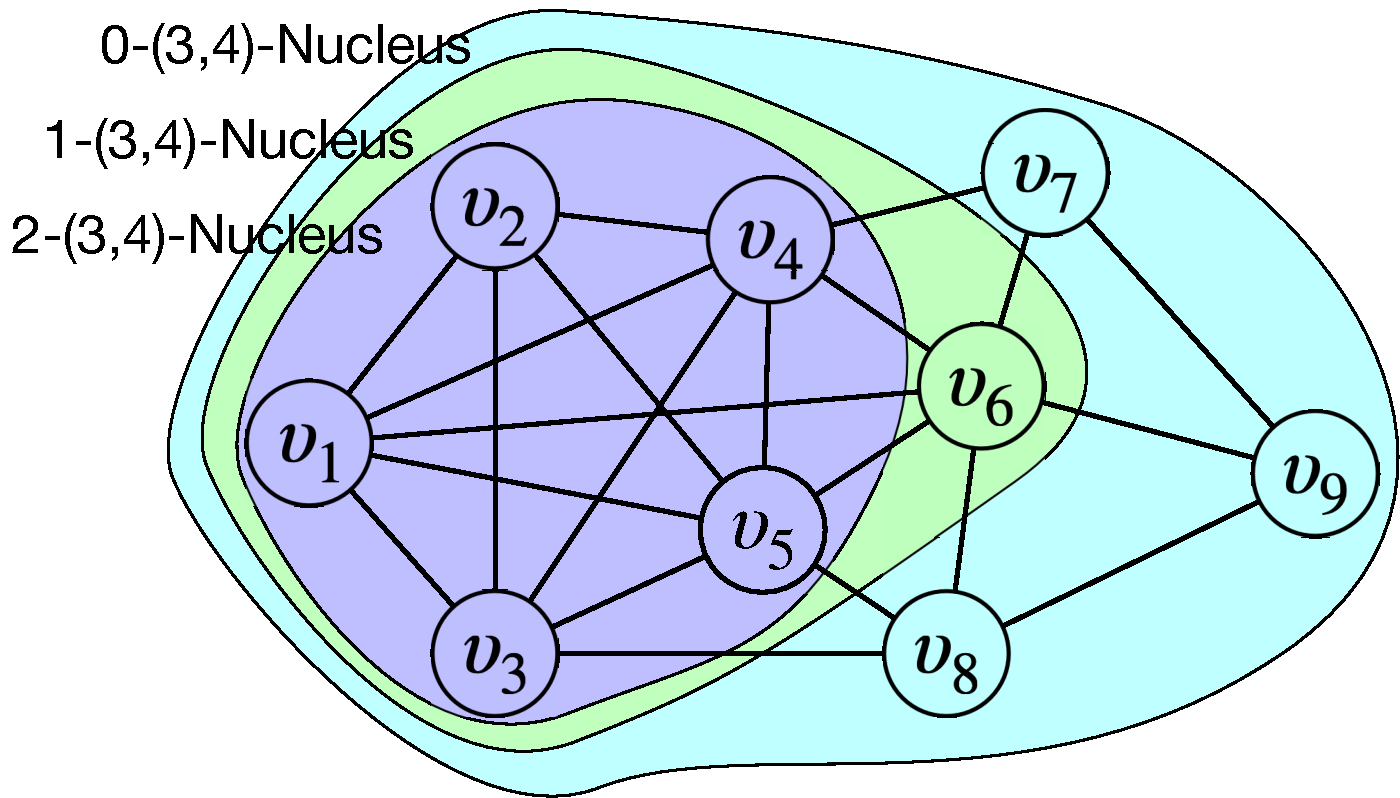
\includegraphics[width=0.32\textwidth]{figure/graph-eps-converted-to.pdf}
    \caption{An example of a graph $G$.}
    \label{fig:graph_example}
\end{figure}

\begin{example}
    Figure~\ref{fig:graph_example} illustrates a sample graph $G$. 
    Taking the $(3,4)$-nucleus as an example, the subgraph induced by vertices $v_1$, $v_2$, $v_3$, $v_4$, and $v_5$ forms a $2$-$(3,4)$-nucleus, as each $3$-clique is contained in at least two $4$-cliques. 
    For instance, the $3$-clique $(v_1, v_2, v_3)$ belongs to the $4$-cliques $(v_1, v_2, v_3, v_4)$ and $(v_1, v_2, v_3, v_5)$. 
    Similarly, all other $3$-cliques in this subgraph satisfy this condition. 
    The maximum nucleus core number for the $(3,4)$-nucleus in this graph is $2$.

    
    % In this graph, we can identify various cliques and analyze their participation in larger cliques to determine the $(r,s)$-nucleus. For instance, the triangle formed by vertices $v_1$, $v_2$, and $v_3$ is a $3$-clique, and we can explore how many $4$-cliques it participates in to compute its nucleus core number. 
    % % 在这个图中, 最大的k-(3,4)-nucleus是由顶点v1, v2, v3, v4, v5组成的2-(3,4)-nucleus, 因为每个3-团都至少包含在2个4-团中. 例如, 3-团(v1, v2, v3)包含在4-团(v1, v2, v3, v4)和(v1, v2, v3, v5)中. 类似地, 其他的3-团也满足这个条件. 因此, 这个图的k-(3,4)-nucleus的核数是2.
    % In this case, the largest $k$-$(3,4)$-nucleus consists of vertices $v_1$, $v_2$, $v_3$, $v_4$, and $v_5$, forming a $2$-$(3,4)$-nucleus since each $3$-clique is contained in at least two distinct $4$-cliques. For example, the $3$-clique $(v_1, v_2, v_3)$ is part of the $4$-cliques $(v_1, v_2, v_3, v_4)$ and $(v_1, v_2, v_3, v_5)$. Similarly, other $3$-cliques in this subgraph also satisfy this condition. Therefore, the nucleus core number for this graph's $k$-$(3,4)$-nucleus is $2$.
\end{example}


% \stitle{Applications.}
% Compared with coherent subgraph models such as the $k$-core and $k$-truss, the $(r,s)$-nucleus provides a more general higher-order model, where $(r,s)$ control cohesiveness. 
% %
% In co-authorship networks, nuclei reveal author groups whose triads repeatedly co-appear in larger cliques, indicating stable collaborations~\cite{newman2001structure,lu2016vital}. 
% %
% In social networks, nuclei highlight tightly knit interaction rings that require multi-actor closure, complementing existing community detection methods~\cite{girvan2002community,ugander2012structural}. 
% %
% In protein-protein interaction and functional networks, nucleus decomposition isolates near-clique modules consistent with biological complex formation~\cite{sharan2006modeling,luo2019higher}. 
% %
% In hyperlink and citation graphs, it identifies cohesive topical clusters~\cite{gleich2012graph,malliaros2013clustering}.


\stitle{Applications.}
% 
Compared with coherent subgraph models such as the $k$-core and $k$-truss, the $(r,s)$-nucleus provides a more general higher-order model, where $(r,s)$ control cohesiveness. 
\myaddRA{
% 
In particular, $r$ specifies the base clique unit, while $s$ specifies the cohesiveness of the resulting nuclei and thus how tightly connected they are.
% 
A larger $s$ imposes a stricter support requirement: an $r$-clique must participate in many distinct $s$-cliques, so nuclei persist only when higher-order overlap is abundant rather than accidental, providing stronger evidence of cohesion~\cite{firstNucleus}.
This requirement arises naturally in many domains; we discuss representative examples below:

% Compared with cohesive subgraph models such as $k$-core and $k$-truss, the $(r,s)$-nucleus is a more general higher-order model in which $r$ selects the base clique unit and $s$ controls the cohesiveness of the resulting nuclei.
% \myaddRA{
% A larger $s$ helps rule out incidental structures by retaining only regions where many $r$-cliques are repeatedly supported by larger clique closures, providing stronger corroboration of cohesion~\cite{firstNucleus}.
% This requirement arises naturally in many domains; we discuss representative examples below:


\sstitle{Coordinated fraud / collusion.}
From interaction logs, we can build a graph where suspicious accounts tend to act in lockstep on many targets.
High-$s$ nuclei help isolate small coordinated rings by filtering out casual triangles and keeping only groups with repeated multi-way coordination~\cite{beutel2013copycatch,hooi2016fraudar}.

\sstitle{Recommendation / e-commerce.}
In an item-to-item graph from co-purchase or co-click signals, high-$s$ nuclei highlight compact bundles of items that co-occur again and again across many users, which can be used as stable and interpretable bundles for browsing, diversification, or cold-start organization~\cite{linden2003amazon}.

\sstitle{Collaboration analysis.}
In a coauthor graph, high-$s$ nuclei capture stable teams whose collaborations are supported by many different higher-order coauthorship cliques, instead of being connected only through one large paper or a single hub author~\cite{newman2001structure}.

% Finally, increasing $r$ is most suitable when the application explicitly requires a minimum mutually connected group size, whereas increasing $s$ controls whether such a group is \emph{repeatedly} corroborated by higher-order interactions~\cite{firstNucleus}.
}


% The parameters $(r,s)$ act as design knobs—$r$ defines the anchor pattern and $s$ specifies the closure requirement—allowing cohesiveness to be tuned to domain semantics. 
%
% These examples illustrate scenarios where higher-order closure, rather than simple pairwise connectivity, is the key structural quantity of interest.
%
%  our counting-based framework enables such analyses at scale without materializing $K_s$.
% The $(r,s)$-nucleus decomposition provides a unifying framework that generalizes classical $k$-core and $k$-truss models, and serves as a foundation for analyzing higher-order structures in large-scale networks~\cite{firstNucleus,seidman1983network,cohen2008trusses}. Its applications span a wide range of domains. In scientific collaboration networks, vertices represent authors and cliques correspond to co-authorship groups. Nuclear decomposition reveals cohesive research communities and identifies influential collaborators~\cite{newman2001structure,lu2016vital}, highlighting long-term, stable collaborations that go beyond simple publication counts. Also, in online social networks, nucleus decomposition uncovers tightly knit groups, key influencers, and hidden community hierarchies~\cite{girvan2002community,ugander2012structural}. By focusing on higher-order structures rather than pairwise interactions, it improves the detection of strong, frequent interactions and enhances the analysis of influence propagation and anomaly detection~\cite{akoglu2015graph}. Similarly, in biological networks, $(r,s)$-nuclei capture protein complexes, metabolic pathways, and functional modules, offering a more accurate representation of molecular interactions than pairwise methods~\cite{sharan2006modeling,luo2019higher}. This enables the discovery of biologically meaningful structures that drive cellular functions. In addition, in the World Wide Web and information networks, nucleus decomposition identifies dense hyperlink-induced subgraphs that represent coherent topical communities~\cite{gleich2012graph, malliaros2013clustering}. These insights can improve web mining, content recommendation, and spam detection by distinguishing interlinked pages from sparse connections.  

% More broadly, nucleus decomposition supports applications in \textbf{network visualization}, where hierarchical dense structures aid in scalable layout design~\cite{huang2014graph}, in \textbf{densest subgraph discovery}~\cite{tsourakakis2013finding}, and in \textbf{network security}, where dense interaction patterns reveal coordinated malicious behaviors~\cite{jiang2016catching}. A particularly important direction is the \textbf{real-time analysis of billion-scale networks}, such as transaction graphs in financial systems, large-scale communication records, or knowledge graphs containing billions of entities and relations. Traditional peeling-based or $h$-index-based frameworks cannot operate in these settings, since explicit enumeration of $s$-cliques or repeated updates of all $r$-cliques are computationally infeasible and memory intensive. Our counting-based framework directly addresses this gap. By replacing clique enumeration with a succinct counting process, it reduces the computational overhead to a scale where continuous updates are possible. The Succinct Clique Tree (SCT) representation compactly encodes the clique space, making support computation feasible even when the underlying graph contains billions of vertices and edges. Furthermore, the framework achieves memory efficiency by avoiding pre-computed clique indices, ensuring that the memory footprint grows linearly with graph size rather than exponentially with clique order. Parallelization further enables decomposition to keep pace with streaming data, which is critical for real-time monitoring.  

% To illustrate, consider a \textbf{financial transaction network} where vertices represent accounts and edges represent money transfers. Higher-order dense subgraphs in this graph may correspond to tightly coordinated transaction groups, which are strong indicators of money laundering, fraudulent trading, or collusive market behavior. In such networks, the volume of daily transactions can reach billions, and new data arrives continuously. Existing decomposition methods cannot scale to this volume, let alone provide timely detection. Our counting-based approach enables the identification of $(r,s)$-nuclei that highlight suspicious clusters in near real time, allowing regulators and financial institutions to react to illicit activities as they occur rather than after significant delays. This scenario demonstrates both the scalability and the practical importance of our framework: it transforms nucleus decomposition from a purely theoretical model into a tool capable of addressing pressing challenges in massive real-world networks.

\stitle{Existing Methods and Key Limitation.} 
Despite its effectiveness and broad applicability, computing nucleus decomposition is computationally intensive, motivating extensive research on improving its efficiency~\cite{sotaHierarchy,sotaPrveHierarchy,LocalNuclear,firstNucleus,nuclearTWEB,nuclearcsonet20}. 
%
Existing studies primarily focus on optimizing the peeling process~\cite{sotaPrveHierarchy,sotaHierarchy}, where the key idea is to iteratively remove low-support $r$-cliques those that participate in fewer $s$-cliques to expose progressively denser substructures. 
%
Other lines of research explore parallel acceleration, either through local update strategies~\cite{LocalNuclear} or multi-threaded peeling algorithms~\cite{sotaPrveHierarchy,sotaHierarchy}. 


However, all existing algorithms share a fundamental limitation: they rely on explicit \textbf{\textit{clique enumeration}}, requiring all $s$-cliques in the graph to be enumerated. 
%
Such enumeration significantly limits scalability, as the number of $s$-cliques increases combinatorially with $s$, often reaching trillion scale even for moderate values of $s$. 
%
As a result, existing approaches are typically limited to small parameter settings (e.g., $(3,4)$-nucleus) or to small and sparse graphs.
%
In theory, the best existing methods achieve asymptotic work complexity comparable to full $s$-clique enumeration~\cite{sotaPrveHierarchy,sotaHierarchy}, leaving the intrinsic computational barrier of explicit clique listing unresolved, particularly for larger graphs and higher parameter values.

% \begin{figure}[t]
%   \centering
%   \begin{subfigure}[b]{0.45\linewidth}
%     \includegraphics[width=\linewidth]{figure/clique_distribution_dblp.eps}
%     \caption{DBLP}
%   \end{subfigure}
%   % \hfill
%   \begin{subfigure}[b]{0.45\linewidth}
%     \includegraphics[width=\linewidth]{figure/clique_distribution_stanford.eps}
%     \caption{web-Stanford}
%   \end{subfigure}
%     \caption{The distribution of $k$-cliques in the datasets. 
%     % The x-axis represents the size of the clique, and the y-axis represents the number of cliques of that size.
%     }
%     \label{fig:clique_distribution}
% \end{figure}

\begin{example}
    The number of $k$-cliques grows explosively with increasing $k$. 
    % Figure~\ref{fig:clique_distribution} shows the clique distribution on the \textsc{DBLP} and \textsc{Stanford} datasets (in Table~\ref{tab:graph-stats}). 
    We observe that in \textsc{DBLP}, the number of $6$-cliques already exceeds $4\times10^9$ and reaches $1.5\times10^{36}$ at $k{=}57$; in \textsc{web-Stanford}, it includes $2.2\times10^{12}$ $28$-cliques.
    Because existing frameworks explicitly enumerate $s$-cliques, the computation becomes quickly infeasible—even enumerating all $6$-cliques alone incurs substantial overhead(Figure \ref{fig:leafcount}).
\end{example}

% The problem is NP-complete, making it challenging to apply to large graphs. Nevertheless, due to its effectiveness and broad applicability, 

% The two prevailing paradigms are: (i) peeling-based methods~\cite{shan2018finding,montresor2013distributed}, which iteratively remove the least-supported $r$-cliques until all remaining satisfy the nucleus condition; and (ii) local $h$-index-based methods~\cite{firstNucleus}, which iteratively update nucleus core numbers by examining neighborhoods of $s$-cliques. While peeling is efficient for small clique sizes, its complexity scales directly with $|K_s|$, the number of $s$-cliques, which is infeasible in practice. The $h$-index method avoids global peeling but requires multiple rounds of iterative updates, each involving expensive neighborhood checks. Both frameworks fundamentally depend on enumerating all $s$-cliques, which prevents them from handling larger $r,s$ values or billion-scale graphs.

\stitle{Research Question.} 
This leads to the critical research question and the main objective of this paper: \textbf{\textit{How to compute $(r,s)$-nucleus decomposition without explicitly enumerating $s$-cliques?}}

\stitle{Challenges.} 
Avoiding $s$-clique enumeration in nucleus decomposition is highly challenging, as enumeration is deeply embedded in all existing algorithmic frameworks.
%
All existing algorithms rely on explicitly enumerating all $s$-cliques for three essential reasons:

% \begin{enumerate}[leftmargin=*]
%     \item \textbf{Computing the support of each $r$-clique:} determining how many $s$-cliques each $r$-clique participates in.
%     \item \textbf{Updating neighboring $r$-cliques during peeling:} when an $r$-clique is removed, the supports of its adjacent $r$-cliques must be updated, which requires access to the shared $s$-cliques.
%     \item \textbf{Defining connectivity between $r$-cliques for hierarchy construction:} hierarchical structures are built based on shared $s$-cliques, again necessitating enumeration.
% \end{enumerate}


\sstitle{Computing the support of each $r$-clique.} 
%
The support of an $r$-clique $R$ is defined as the number of $s$-cliques containing it. 
Existing methods compute this by enumerating all $s$-cliques and recording, for each $r$-clique, the set of $s$-cliques that include it.

\sstitle{Updating neighboring $r$-cliques during peeling.} 
When an $r$-clique $R$ is removed during the peeling process (along with all $s$-cliques containing it), every $r$-clique $R'$ that shares an $s$-clique with $R$ must have its support decremented by $1$. 
This update requires knowing, for each $s$-clique, the set of $r$-cliques it contains; thus, adjacency among $r$-cliques is derived from enumerated $s$-cliques.

\sstitle{Defining connectivity for hierarchy construction.}
%
Two $r$-cliques $R$ and $R'$ are \emph{$s$-connected} if a sequence of $r$-cliques exists such that each consecutive pair of cliques shares at least one common $s$-clique. 
To identify nucleus components for hierarchy construction, existing algorithms enumerate and traverse all $s$-cliques to determine these connectivity relationships.


% However, all existing approaches share a fundamental limitation: they are \textbf{enumeration-based}, requiring explicitly enumerating all $s$-cliques in the graph. This significantly restricts their scalability to large graphs and higher value of $s$.
% % \todo{why do existing methods enumerate s-cliques? why is it (\textbf{fundamentally}) hard to compute $(r,s)$-nucleus without enumeration? }
% % Unlike pairwise cores where degrees provide simple update rules, nucleus decomposition requires enumerating all $s$-cliques to compute the $(r,s)$-support of each $r$-clique. 
% Exact $(r,s)$-support for an $r$-clique equals the number of $s$-cliques containing it. Without a counting oracle, the only general way to obtain and maintain these supports during peeling is to materialize (or re-enumerate) the incident $s$-cliques. Supports are not functions of local degrees: an $r$-clique can form $s$-cliques through many overlapping, non-local neighborhoods, so deletions propagate widely. Hence existing frameworks reduce exact maintenance to listing or indexing $K_s$, which leads to combinatorial blow-up as $s$ increases.

% Unlike pairwise cores where degrees provide simple update rules, nucleus decomposition requires enumerating all $s$-cliques to compute the $(r,s)$-support of each $r$-clique. 
 
% We identify three major bottlenecks:

% \sstitle{Clique enumeration overhead.}  
% A principal difficulty arises from the reliance on enumerating all $s$-cliques in order to compute the support of each $r$-clique. Since the number of $s$-cliques grows combinatorially with graph size and clique order, this step dominates the runtime of existing algorithms. The enumeration overhead fundamentally restricts scalability and makes nucleus decomposition infeasible for large graphs or higher-order parameters. Overcoming this challenge is crucial to enable algorithms that avoid explicit enumeration and can operate efficiently on complex networks.  

% \sstitle{Inefficient counting maintenance.}  
% The core difficulty is not maintaining the cliques themselves, but maintaining the \emph{counting} of $s$-cliques per $r$-clique as the decomposition progresses. When one $r$-clique is removed, every $s$-clique containing it becomes invalid, and consequently the counting of all other $r$-cliques in those $s$-cliques must be decremented. Existing approaches attempt to handle this either by re-enumerating affected $s$-cliques\cite{fastHierarchy,LocalNuclear}, which causes massive redundancy and wasted computation, or by storing explicit mappings from each $r$-clique to all of its incident $s$-cliques, which requires frequent updates. Neither approach provides a scalable solution. Current frameworks therefore lack a compact, update-friendly representation that can deliver correct support deltas without exhaustive neighborhood scans. Overcoming this limitation is critical, since accurate and selective maintenance of counting is the prerequisite for enabling nucleus decomposition to scale to large graphs and higher-order parameters.

% \sstitle{Lack of hierarchical exploitation.}  
% Nuclear decomposition is inherently hierarchical: an $(r,s)$-nucleus is nested within higher-order structures, and computing deeper levels of the decomposition depends on accurate values at shallower levels. Existing algorithms cannot fully exploit this hierarchy, because their reliance on enumeration and updates prevents reusing intermediate results across levels. Thus, they recompute supports from scratch for each stage, incurring exponential computation time. The inability to maintain and propagate hierarchical information has been a critical bottleneck in applying nucleus decomposition to large, complex graphs. 

\stitle{Our Idea.} 
% Inspired by the advances in clique counting~\cite{Pivoter}, 
To efficiently support the above core operations of nucleus decomposition while avoiding explicit $s$-clique enumeration, we design a novel auxiliary data structure, the \textit{Clique Path Index} (\cpi), 
%
% maximial clique enumeration should be mentioned somewhere?
\cpi encodes the space of $s$-cliques into compact paths, enabling counting, updates, and connectivity queries to be executed directly over these paths without enumeration. 
%
The proposed index provides the following key features:

\sstitle{Counting without enumeration.} 
%
\cpi enables $s$-clique counting and the computation of $r$-clique supports by aggregating path statistics, thereby avoiding the exponential overhead of enumerating all $s$-cliques as in existing algorithms.

\sstitle{Dynamic and efficient updates.} 
%
\cpi performs efficient incremental updates during peeling by dynamically modifying or splitting affected clique paths upon deletions.
As clique information is aggregated in the path representation, removing a single $r$-clique implicitly accounts for the removal of many $s$-cliques, thereby significantly reducing redundant computation during peeling.

\sstitle{Built-in connectivity maintenance.} 
%
\cpi maintains $s$-connectivity naturally among $r$-cliques during updates. 
Connectivity relationships are preserved and adjusted within the indexed paths, enabling hierarchy construction to be performed directly without additional traversal or re-enumeration.

\sstitle{From index design to differential maintenance.}
%
While \cpi resolves the representation problem, the remaining algorithmic challenge is how to maintain exact supports during peeling without reverting to local re-materialization.
%
Our journal-level view is that nucleus peeling on \cpi is fundamentally a \emph{differential path contribution maintenance} problem:
each path contributes a local amount of support to the $r$-cliques it covers, and after a peeling round only the contributions on paths incident to removed $r$-cliques can change.
%
This perspective isolates the true source of efficiency gains beyond the index itself and explains why different regimes of $r$ admit different exact update mechanisms.


% 1. Computing the Support of Each $r$-Clique -> counting
% 2. Updating Neighboring $r$-Cliques (during the Peeling Process) -> remove redundant computation
% 3. Defining Connectivity Between $r$-Cliques (Hierarchy Construction) -> filtering 


\stitle{Contributions.} 
Building on the proposed \textit{Clique Path Index} (\cpi), we present a counting-based nucleus decomposition framework.
%
We also present a higher-level differential maintenance theory for exact peeling.
%
The main contributions of this work are summarized as follows:

\sstitle{Counting-based nucleus decomposition via the Clique Path Index.}
%
We propose a compact path-based representation of the $s$-clique search space that avoids explicit $s$-clique enumeration while still supporting exact support counting, dynamic updates, and hierarchy construction.
%
This is the representation layer of our method.

\sstitle{A differential path contribution maintenance theory.}
%
We formalize nucleus peeling on \cpi as maintaining path-local support contributions under deletions.
%
Under this view, the support of each active $r$-clique is the sum of path contributions.
%
After each peeling round, only paths incident to removed $r$-cliques need updates.

\sstitle{Exact regime-specific update operators for $r{=}1$, $r{=}2$, and $r{\ge}3$.}
%
Under the differential maintenance view, we derive three exact specialized instantiations:
counter-only path maintenance for $r{=}1$,
closed-form deltas and analytical single-edge splits for $r{=}2$,
and dead-path-aware lazy maintenance for $r{\ge}3$.
%
These instantiations show how the same framework leads to different update operators in different regimes.

\sstitle{Integrated hierarchy construction and comprehensive evaluation.}
%
Our method naturally preserves $s$-connectivity among $r$-cliques within \cpi, enabling hierarchy construction with minimal extra overhead.
%
Experiments show clear gains over prior methods.
%
On comparable settings, our method is about $4\times$ faster than \arb and about $13\times$ to $27\times$ faster than the \nucleus baselines.
%
On some instances, the speedup exceeds two orders of magnitude.
%
The gains hold for both decomposition and hierarchy construction.

\sstitle{Extension over the conference version.}
%
Compared with the conference version of this work, this journal version makes three substantive extensions.
%
First, it introduces the differential path contribution maintenance formalism.
%
This formalism isolates the exact support-update primitive beyond the index itself.
%
Second, it derives regime-specific sufficient states and exact update operators for $r{=}1$, $r{=}2$, and $r{\ge}3$.
%
These operators follow one common maintenance principle.
%
Third, it strengthens the optimization and complexity analysis.
%
It explains how different peeling regimes reduce update costs without losing exactness.

\stitle{Organization.}
%
Section~\ref{sec:preliminaries} reviews the problem definition and notation.
%
Section~\ref{sec:existing_approaches} revisits the peeling baseline and motivates avoiding explicit $s$-clique enumeration.
%
Section~\ref{sec:our_approach} introduces the representation layer through \cpi.
%
Section~\ref{sec:dpcm} then lifts it to a differential path contribution maintenance view.
%
Section~\ref{sec:update_cpi} then instantiates this view for general $r{\ge}3$, for $r{=}2$, and for $r{=}1$, followed by dead-path-aware refinements.
%
The remaining sections present hierarchy construction, experiments, case studies, and related work.


% 

% All prior algorithms for nucleus decomposition have been tied to explicit enumeration, either constructing every $s$-clique in advance or re-enumerating them during updates. This reliance on enumeration has been the fundamental scalability barrier, as the number of $s$-cliques grows combinatorially with graph size and clique order. We present the first \emph{counting-based} framework for nucleus decomposition, which replaces explicit enumeration with direct clique-counting operations over the Succinct Clique Tree (SCT). This breakthrough eliminates the exponential dependence on $s$-clique enumeration and allows supports to be computed and maintained in closed form. As a result, our framework makes it possible, for the first time, to perform nucleus decomposition at higher-order parameters and on graph scales that were previously infeasible. This shift from enumeration to counting marks a fundamental change in how nucleus decomposition is designed and establishes a new foundation for scalable higher-order graph analysis.


% \sstitle{First efficient update mechanism.}
% Prior algorithms for nucleus decomposition lacked any practical way to maintain support counts incrementally. They relied on recomputation or full re-enumeration of affected cliques, which introduced massive redundancy and prevented scalability. We provide the first efficient update mechanism by leveraging the Succinct Clique Tree (SCT) together with clique-counting formulas and pruning strategies. This mechanism updates supports selectively and maintains the tree incrementally, avoiding reconstruction of local substructures. As a result, nucleus decomposition is no longer bound to costly iterative recomputation but can instead be performed with efficient, scalable updates, making the method practical for massive real-world graphs.

% \sstitle{Succinct data structure for counting.}  
% Existing algorithms for nucleus decomposition lack any data structure that can maintain clique counts compactly and update them efficiently. The state-of-the-art methods either re-enumerate all affected cliques after every deletion, incurring prohibitive overhead, or store explicit mappings from each $r$-clique to its incident $s$-cliques, which quickly becomes infeasible in memory. We introduce the first SCT-based data structure that encodes the entire clique space in a compressed, lossless representation. This structure supports direct counting of $s$-cliques containing any $r$-clique without explicit enumeration, and it enables incremental updates during decomposition without scanning large neighborhoods. By combining compactness with update efficiency, the SCT data structure resolves a long-standing bottleneck in nucleus decomposition: how to maintain counting information at scale. This innovation provides the theoretical foundation and practical backbone that makes our counting-based framework possible, and represents a significant departure from all previous approaches.
 

% \sstitle{Hierarchy without prior knowledge of $s$.} \ A key advantage of our framework is that it can compute the full hierarchy of nucleus structures without requiring $s$ to be fixed in advance. Existing state-of-the-art methods typically recompute supports separately for each choice of $s$, which is costly and inflexible. By contrast, our approach leverages the Succinct Clique Tree (SCT) representation to decide $s$-connectivity. This property allows us to identify nuclei hierarchically across all possible values of $s$ in a unified manner. To maintain this hierarchy efficiently during decomposition, we employ a multi-level disjoint set union (DSU) structure in which each level corresponds to a $k$-core. This design ensures that once two $r$-cliques are merged at a given level, they remain merged in all smaller levels, thereby preserving containment relationships. As a result, our framework constructs the entire nucleus hierarchy dynamically and incrementally, eliminating the need for recomputation at different values of $s$. This capability is crucial for large-scale analysis, as it enables flexible exploration of higher-order structures even when the appropriate $s$ is not known beforehand.





% \sstitle{Comprehensive experimental validation.}  
% We conduct an extensive set of experiments on real-world datasets of varying scale and density. Our work advances the state-of-the-art by moving beyond previous time-outs, enabling efficient computation and obtaining results on comparatively large graphs. These improvements validate the effectiveness of our framework across different application domains. They show that our approach not only advances the theoretical state-of-the-art but also provides a practical solution that can be immediately applied in large-scale graph analysis.

\myaddRC{\section{Preliminaries}\label{sec:preliminaries}
}
% In this section, we introduce the graph notation and the definitions used to compute per‑clique $(r,s)$‑core numbers; hierarchy/connected components are deferred to later sections.

%--------------------------------------------------
% 符号表
%--------------------------------------------------
% \begin{table}[ht]
%   \centering
%   \caption{Notation used throughout the paper}\label{tab:notation}
%   \begin{tabular}{ll}
%     \hline
%     \textbf{Symbol} & \textbf{Meaning}\\
%     \hline
%     $G=(V,E)$     & simple, unweighted graph \\
%     $G[V']$       & subgraph of $G$ induced by $V' \subseteq V$\\
%     $n = |V|$     & \#vertices of $G$\\
%     $m = |E|$     & \#edges of $G$\\
%     $\deg(v)$     & degree of vertex $v$\\
%     $C\subseteq V$ & a clique (context specifies its size)\\
%     $\deg_{(s)}(R)$ & $s$-clique degree of an $r$-clique $R$ in $G$\\
%     $G_k$         & a $k$-\((r,s)\)-nucleus (defined below)\\
%     $\kappa_{s}(R)$ & \((r,s)\)-nucleus core number of $r$-clique $R$\\
%     \hline
%   \end{tabular}
% \end{table}

%--------------------------------------------------
% 基本概念
%--------------------------------------------------
\stitle{Graph Notations.} 
We focus on a \emph{simple}, \emph{unweighted} graph, defined as a pair $G=(V,E)$ where $V$ is the set of vertices and $E\subseteq V\times V$ is the set of undirected edges. 
%
We use $N_G(v)=\{u\in V \mid (u,v)\in E\}$ to denote the set of neighbors of a vertex $v\in V$ in $G$, and $\deg_G(v)=|N_G(v)|$ to denote its degree.
% 
We use $G[V']$ to denote the subgraph \emph{induced} by a vertex subset $V'\subseteq V$. 
%
We store a graph $G$ in the classical Compressed Sparse Row (CSR) format, consisting of two integer arrays: \texttt{offsets} of length $|V|{+}1$ and \texttt{edges} of length $|E|$.

\begin{definition}[$k$-Clique]\label{def:k-clique}
A \emph{$k$-clique} is a vertex set $C\subseteq V$ with $|C|=k$ such that $(u,v)\in E$ for every $u,v\in C$. 
\end{definition}

% \begin{example}
%     Each vertex is a $1$-clique, each edge is a $2$-clique, and each triangle is a $3$-clique.
% \end{example}

\begin{definition}[$(r,s)$-Clique Degree]\label{def:r-s-degree}
Given two integers $0 < r < s$, 
the \emph{$(r,s)$-clique degree} of an $r$-clique $R$ in $G$ is defined as
\[
  \deg_{(s)}^{G}(R)
  \;=\;
  \bigl|\,\{\,S \subseteq V \mid R \subseteq S, \; S \text{ is a } s\text{-clique in } G\,\}\,\bigr|.
\]
\end{definition}
% 说一下这个也叫做 $s$-clique support
We also refer to $\deg_{(s)}^{G}(R)$ as the \emph{$s$-clique support} of $R$ in $G$.
When the graph $G$ is clear from the context, we simply write $\deg_{(s)}(R)$.

%--------------------------------------------------
% nucleus 核心定义
%--------------------------------------------------

% \begin{definition}[{$k$-admissible $s$-clique}]
% Given integers $0<r<s$ and $k>0$.  
% An induced $s$-clique $S$ in $G$ is called \emph{$k$-admissible}
% if every $r$-clique $R\subseteq S$ satisfies $\deg_{(s)}(R)\ge k$.
% \end{definition}

\begin{definition}[{$k$-admissible $s$-clique}]
Given integers $0 < r < s$ and $k > 0$,  
an induced $s$-clique $S$ in $G$ is called \emph{$k$-admissible} 
if every $r$-clique $R \subseteq S$ satisfies $\deg_{(s)}(R) \ge k$.
\end{definition}


% \begin{definition}[{$r$-clique-support}]
% The \emph{$r$-clique-support} of an $s$-clique $S$ in $G$ is defined as
% \end{definition}

\begin{definition}[$k$-$(r,s)$-nucleus]\label{def:k-rs-nucleus-new}
Let $\mathcal S_k$ be the set of all $k$-admissible $s$-cliques of $G$.
For any subset $\mathcal S\subseteq\mathcal S_k$, denote
$
   G[\mathcal S] \;=\; G\, \!\Bigl[\,
        \bigcup_{S\in\mathcal S} S
   \Bigr].
$
A subgraph $G_k = G[\mathcal S]$ is a \emph{$k$-$(r,s)$-nucleus} if
\begin{enumerate}[leftmargin=*]
  \item $G_k$ is \emph{$s$-connected}: for any two $r$-cliques
        $R,R'\subseteq V(G_k)$, there is a sequence
        $R=R_1,\dots,R_t=R'$ with
        $R_i\cup R_{i+1}\subseteq S_i$ for some
        $S_i\in\mathcal S$;
  \item $G_k$ is \emph{maximal}, i.e., no proper superset
        $\mathcal{S}' \supset \mathcal{S}$ still satisfies condition~(1).
\end{enumerate}
\end{definition}

% \stitle{Intuition.}
A $k$-$(r,s)$-nucleus is a maximal subgraph in which 
every $r$-clique participates in at least $k$ distinct $s$-cliques, 
and all such $r$-cliques are tightly connected through shared $s$-cliques. 
% The formal definition is given below.

\begin{definition}[Core Number]\label{def:r-clique-core-number}
Given two integers $0 < r < s$,  
the \emph{$(r,s)$-nucleus core number} (or \textit{coreness}) of an $r$-clique $R$, denoted by $\kappa_s(R)$, 
is the largest integer $k$ such that there exists a $k$-$(r,s)$-nucleus $G_k$ in $G$ containing $R$. 
Equivalently, it is the largest integer $k$ for which $R$ belongs to some $k$-$(r,s)$-nucleus $G_k$ in $G$.
\end{definition}

%--------------------------------------------------
% s-clique connectivity
%--------------------------------------------------
% \begin{definition}[$s$-Connectivity]\label{def:s-connect}
% Fix integers $0<r<s$.  
% Two $r$-cliques $R$ and $R'$ in a graph (or subgraph) $H$ are \emph{$s$-connected}
% if there exists a sequence of $r$-cliques
% $
%   R=R_1, R_2, \dots, R_t=R'
% $
% such that for each $i\in\{1,\dots,t-1\}$ there is an induced $s$-clique
% $S_i\subseteq V(H)$ with $R_i\cup R_{i+1}\subseteq S_i$.
% The sequence $\langle R_1,\dots,R_t\rangle$ is called an \emph{$s$-clique path}.
% \end{definition}

% \begin{definition}[$s$-Connected Component]\label{def:s-component}
% For fixed $0<r<s$, the \emph{$s$-connected component} of an $r$-clique
% $R$ (with respect to $s$) is the vertex-induced subgraph
% \[
%   \mathrm{Comp}_s(R) \;=\;
%   G\!\Bigl[\,
%     \bigcup_{R'\,:\;R'\text{ is }s\text{-connected to }R} R'
%   \Bigr].
% \]
% Equivalently, it is the maximal subgraph $H$ containing $R$
% such that any two $r$-cliques in $H$ are $s$-connected within $H$.
% $s$-Connectedness is an equivalence relation on the set of $r$-cliques; hence
% $s$-connected components form a partition of all $r$-cliques in $G$.
% \end{definition}

\sstitle{Problem statement.}
Given a graph $G$ and integers $0 < r < s$, the goal is to compute the $(r,s)$-nucleus core number $\kappa_s(R)$ for every $r$-clique $R$ in $G$. (The hierarchy construction of $k$-$(r,s)$ nuclei will be formally discussed in Section~\ref{sec:hierarchy}.)



% 
% \section{Existing Approaches}

% In this section, we review existing approaches for nucleus core decomposition and discuss their limitations. 
% %
% We focus on the classical peeling-based framework for nucleus decomposition~\cite{firstNucleus,fastHierarchy,sotaPrveHierarchy,sotaHierarchy, nuclearTWEB}. 
% Although local update-based methods~\cite{LocalNuclear} have also been proposed to enable parallel computation, they share the same fundamental limitation of explicit $s$-clique enumeration and are therefore not discussed in detail here due to page limit.

% \begin{algorithm}[t]
\small
\caption{Peeling Framework}
\label{alg:peel_concept}
\KwIn{Graph $G$, clique sizes $0<r<s$}
\KwOut{$\kappa_s(R)$ for every $r$-clique $R$}

%-------------------------
% Step 1 : initial counts
%-------------------------
% $mark$ every $r$-clique $R \in G$ as \texttt{active};
Enumerate all $r$-cliques in $G$;

Enumerate all $s$-cliques in $G$;

$mark$ every $s$-clique $S \in G$ as \texttt{active};


$\delta(R)\leftarrow$ the number of $s$-cliques that contain $R$

$coreness \leftarrow 0$

%-------------------------
% Step 2 : peeling loop
%-------------------------
\While{there exists \texttt{active} $r$-cliques}{
    find $c=\min\{\delta(R)\mid R\text{ is \texttt{active}}\}$

    $coreness \leftarrow max(c, coreness)$

    let $\mathcal{R}=\{R\mid \delta(R)=c,\;R\text{ \texttt{active}}\}$

    \ForEach{$R\in\mathcal{R}$}{
        $\kappa_s(R)\leftarrow coreness$

        mark $R$ as \texttt{inactive};

        \ForEach{\texttt{active} $s$-clique $S$ with $R\subseteq S$}{
            mark $S$ as \texttt{inactive};

            \ForEach{\texttt{active} $r$-clique $R'\subseteq S$}{
                $\delta(R')\leftarrow\delta(R')-1$;
            }
        }
    }
}
\Return{$\kappa_s(R)$ for every $r$-clique $R \in G$}
\end{algorithm}


% \begin{algorithm}[t]
\small
% \caption{\textsc{Local $h$-Index Framework}}
% \label{alg:hindex_concept}
% \KwIn{Graph $G$, clique sizes $0<r<s$}
% \KwOut{$\\\kappa_s(R)$ for every $r$-clique $R$}

% $\\\kappa_s(R) \leftarrow |nbr_s(R)|$ for every $r$-clique $R \in G$

% $update \leftarrow$ \texttt{true}

% \While{$update$}{
%     $update \leftarrow \texttt{false}$\;

%     \ForEach{$r$-clique $R$ in $G$}{
%         $L \leftarrow [\,]$

%         \ForEach{$s$-clique $S$ with $R\subseteq S$}{
%             $m_S \leftarrow \min_{R'\subseteq S,\;R'\neq R}\kappa(R')$\;
%             append $m_S$ to $L$\;
%         }

%         $\kappa^{new}(R) \leftarrow \mathcal{H}(L)$\;
%         \If{$\kappa^{new}(R) \neq \kappa(R)$}{
%             $\kappa(R) \leftarrow \kappa^{new}(R)$\;
%             $update \leftarrow \texttt{true}$\;
%         }   
%     }
% } 

% \Return{$\\\kappa_s(R)$ for every $r$-clique $R \in G$}

% \end{algorithm}


% % Peeling是最被广泛使用的Nuclear Core Decomposition方法, 其基本思想是通过逐层剥离（peeling）图中的拥有最少s-clique的r-clique来计算每个r-clique的coreness.在每一轮中，算法都会找到所有的活跃r-clique，并将其剥离，直至没有活跃的r-clique为止。
% Algorithm~\ref{alg:peel_concept} illustrates the basic paradigm of peeling-based algorithms. 
% It computes the coreness of each $r$-clique by iteratively peeling off the $r$-cliques with the smallest number of associated $s$-cliques in each round. 
% In every iteration, the algorithm identifies all active $r$-cliques and removes them until no active $r$-cliques remain.
% % 算法\ref{alg:peel_concept}展示了Peeling的基本框架.

% The peeling framework comprises two phases: \emph{initial counting} and the \emph{peeling loop}. 
% In the initial counting phase, all $r$-cliques and $s$-cliques are enumerated and marked as active, and the number of active $s$-cliques containing each active $r$-clique is computed. 
% In the peeling loop, the algorithm iteratively identifies and removes active $r$-cliques with the smallest number of active $s$-cliques; 
% the $s$-cliques containing these $r$-cliques are then marked as inactive. 
% This process continues until no active $r$-cliques remain. 
% The coreness of each $r$-clique is assigned to the current peeling level, which corresponds to the minimum number of active $s$-cliques containing that $r$-clique.

% % O(|K_r|+|K_s|)
% \stitle{Complexity.} 
% The time complexity of the peeling framework is $O(|K_r| + |K_s|)$ \cite{sotaPrveHierarchy}, where $|K_r|$ and $|K_s|$ represent the numbers of $r$-cliques and $s$-cliques in the graph, respectively .

% \stitle{Clique Enumeration in Existing Approaches.}
% Existing methods have time and space complexities that rely on the total number of $s$-cliques in the graph. 
% However, the number of $s$-cliques grows combinatorially with $s$, leading to prohibitive computational costs. 
% As a result, current algorithms fail to scale to larger $s$ values, with state-of-the-art methods handling only small configurations (e.g., $(4,5)$-nucleus decomposition) on small or sparse datasets. 
% Hence, it is essential to revisit the algorithm design to remove this dependency and avoid explicit enumeration of $s$-cliques.
\myaddRC{
Computing these core numbers requires tracking, for each $r$-clique $R$, its \emph{active} $s$-clique support $\deg_{(s)}(R)$ (Definition~\ref{def:r-s-degree}) under a sequence of deletions.
A widely used approach in prior work is the peeling-based nucleus decomposition~\cite{firstNucleus,fastHierarchy,sotaPrveHierarchy,sotaHierarchy,nuclearTWEB}:
starting from the full graph, it iteratively removes the active $r$-cliques with the smallest current support and updates the supports of the remaining $r$-cliques.
We summarize this baseline next to fix terminology and to expose the scalability bottleneck that motivates our index-based design.

\begin{algorithm}[t]
\small
\caption{Peeling Framework}
\label{alg:peel_concept}
\KwIn{Graph $G$, clique sizes $0<r<s$}
\KwOut{$\kappa_s(R)$ for every $r$-clique $R$}

%-------------------------
% Step 1 : initial counts
%-------------------------
% $mark$ every $r$-clique $R \in G$ as \texttt{active};
Enumerate all $r$-cliques in $G$;

Enumerate all $s$-cliques in $G$;

$mark$ every $s$-clique $S \in G$ as \texttt{active};


$\delta(R)\leftarrow$ the number of $s$-cliques that contain $R$

$coreness \leftarrow 0$

%-------------------------
% Step 2 : peeling loop
%-------------------------
\While{there exists \texttt{active} $r$-cliques}{
    find $c=\min\{\delta(R)\mid R\text{ is \texttt{active}}\}$

    $coreness \leftarrow max(c, coreness)$

    let $\mathcal{R}=\{R\mid \delta(R)=c,\;R\text{ \texttt{active}}\}$

    \ForEach{$R\in\mathcal{R}$}{
        $\kappa_s(R)\leftarrow coreness$

        mark $R$ as \texttt{inactive};

        \ForEach{\texttt{active} $s$-clique $S$ with $R\subseteq S$}{
            mark $S$ as \texttt{inactive};

            \ForEach{\texttt{active} $r$-clique $R'\subseteq S$}{
                $\delta(R')\leftarrow\delta(R')-1$;
            }
        }
    }
}
\Return{$\kappa_s(R)$ for every $r$-clique $R \in G$}
\end{algorithm}


% \begin{algorithm}[t]
\small
% \caption{\textsc{Local $h$-Index Framework}}
% \label{alg:hindex_concept}
% \KwIn{Graph $G$, clique sizes $0<r<s$}
% \KwOut{$\\\kappa_s(R)$ for every $r$-clique $R$}

% $\\\kappa_s(R) \leftarrow |nbr_s(R)|$ for every $r$-clique $R \in G$

% $update \leftarrow$ \texttt{true}

% \While{$update$}{
%     $update \leftarrow \texttt{false}$\;

%     \ForEach{$r$-clique $R$ in $G$}{
%         $L \leftarrow [\,]$

%         \ForEach{$s$-clique $S$ with $R\subseteq S$}{
%             $m_S \leftarrow \min_{R'\subseteq S,\;R'\neq R}\kappa(R')$\;
%             append $m_S$ to $L$\;
%         }

%         $\kappa^{new}(R) \leftarrow \mathcal{H}(L)$\;
%         \If{$\kappa^{new}(R) \neq \kappa(R)$}{
%             $\kappa(R) \leftarrow \kappa^{new}(R)$\;
%             $update \leftarrow \texttt{true}$\;
%         }   
%     }
% } 

% \Return{$\\\kappa_s(R)$ for every $r$-clique $R \in G$}

% \end{algorithm}

\stitle{Baseline: Peeling-Based Nucleus Decomposition.}\label{sec:existing_approaches}
% 
Algorithm~\ref{alg:peel_concept} illustrates the peeling paradigm.
In the \emph{initial counting} phase, all $r$-cliques and $s$-cliques are enumerated and marked active, and each active $r$-clique $R$ is assigned its initial support $\deg_{(s)}(R)$.
In the peeling loop, the algorithm repeatedly removes the active $r$-cliques with the smallest support;
then every active $s$-clique that contains a removed $r$-clique is marked inactive, which decreases the support of the remaining $r$-cliques that it contains.
The coreness $\kappa_s(R)$ of each $r$-clique is the peeling level at which it is removed.

This framework runs in $O(|K_r| + |K_s|)$ time~\cite{sotaPrveHierarchy}, where $|K_r|$ and $|K_s|$ denote the numbers of $r$-cliques and $s$-cliques, respectively.
However, both time and space critically depend on \emph{explicitly enumerating} $s$-cliques (during initial counting and during support updates).
Since $|K_s|$ can grow combinatorially with $s$, this dependence quickly becomes prohibitive as $s$ increases, which explains why prior methods typically target only small configurations (e.g., $(4,5)$-nucleus) on small or sparse graphs.
Local update-based variants have been proposed to improve parallelism~\cite{LocalNuclear}, but they still rely on $s$-clique enumeration and thus inherit the same bottleneck.
These limitations motivate algorithmic designs that avoid explicit $s$-clique enumeration.

\stitle{Baseline Primitive: Eager Support Maintenance.}
The reference methods in our experiments differ in implementation details.
%
However, they share the same exact peeling skeleton.
%
They repeatedly remove minimum-support active $r$-cliques.
%
They then maintain exact supports for the surviving $r$-cliques.
%
The key difference lies in the \emph{support-maintenance primitive}.
%
In prior methods, support maintenance is eager.
%
When a peeled unit invalidates incident $s$-cliques, the algorithm either enumerates the affected $s$-cliques or reconstructs the affected local structure.
%
It then recomputes the supports.
%
This primitive is \emph{reconstructive}.
%
It materializes or revisits local clique structure after each update.

\stitle{From Reconstructive to Differential Maintenance.}
Our journal-level goal is not to replace the exact peeling skeleton.
%
Our goal is to replace the reconstructive maintenance primitive.
%
The \cpi gives a compact counting representation.
%
DPCM shows how to update exact supports by \emph{differential path contribution updates}.
%
That is, we update only the local path states incident to removed units.
%
We do not re-materialize the affected $s$-clique space.
%
This point is important.
%
Our novelty is not a new decomposition paradigm.
%
Our novelty is a new exact support-maintenance theory under the same decomposition paradigm.
}

\section{The Representation Layer: Clique Path Index} \label{sec:our_approach}

% 我们的算法的核心思想是通过对于每一个$r$-clique计算其$s$-clique的个数来进行计算, 无需枚举任何$s$-clique, 只需要知道数量即可. 
In this section, we present the representation layer of our method for nucleus decomposition, which addresses the limitations of existing methods by eliminating their reliance on explicit $s$-clique enumeration. 
%
The key idea of our algorithm is to leverage the proposed \textit{Clique Path Index} (\cpi) to directly count $s$-cliques while maintaining and updating the index dynamically during the peeling process. 
%
In the following, we first provide an overview of this counting/indexing layer, then review the background on clique counting, and finally present the definition and design of \cpi.


\subsection{Overview}
% \begin{algorithm}[t]
\small
% \caption{\textsc{$(r,s)$-CND}}
% \label{alg:framework}
% \KwIn{Clique size $s$}
% \KwOut{Core value $\kappa_s(v)$ for every vertex $v$}
% \SetKwFunction{RemoveNode}{RemoveNode}
% \SetKwFunction{CountPreEdges}{$s$-CliqueCount}
% \SetKwProg{Fn}{Function}{:}{}

% $\tree$ $\leftarrow$ build CPI of $G$, pruning paths with $s$\;

% $support \gets$ \textsc{CountPreEdges}$(\mathcal{B}, r, s)$\;

% build min heap $H_{\min}$ using $support$\;

% $c_{min} \gets 0$\;

% \While{$H_{\min}$ is not empty}{
%     $R_{min} \gets \text{ExtractMin}(H_{\min})$\;
%     $c_{min} \gets \max(c_{min}, support(R_{min}))$\;
%     $\kappa_s(R_{min}) \gets c_{min}$\;
%     \ForEach{leaf $\TPath$ intersecting any $rc \in R_{min}$}{
%         $B \gets {\,rc \in R_{min} \mid rc \in \TPath\,}$\;
%         \text{Remove all $r$-cliques in $B$ from $\TPath$}\;
%     }

%     \ForEach{leaf $\TPath$ containing any $rc \in R_{min}$}{
%         Update $support(rc)$ and $H_{\min}$ for all $r$-clique $rc \in \TPath$
%     }

% }

% \Return{$\kappa_s(r)$ for all $r$-cliques $r$ in $\tree$}\;

% \end{algorithm}

\begin{algorithm}[t]
\small
\caption{\textsc{$(r,s)$-\cbnd}}
\label{alg:framework}
\KwIn{Graph $G=(V,E)$, clique sizes $r<s$}
\KwOut{Core value $\kappa_s(R)$ for every $r$-clique $R$}
\SetKwFunction{RemoveNode}{RemoveNode}
\SetKwFunction{CountPreEdges}{$s$-CliqueCount}
\SetKwProg{Fn}{Function}{:}{}

$\tree \leftarrow \textsc{BuildIndex}(G)$\;

\tcp{initialize $s$-support for all $r$-cliques}

$support \gets$ \textsc{$s$-CliqueCount}$(\tree, r, s)$ 

build a min-heap $H_{\min}$ using $support$\;

$c_{min} \gets 0$\;

\While{$H_{\min}$ is not empty}{
    $R_{min} \gets \text{ExtractMin}(H_{\min})$\;
    $c_{min} \gets \max(c_{min}, support(R_{min}))$\;
    $\kappa_s(R_{min}) \gets c_{min}$\;
    
    % remove $R_{min}$ from index
    % Remove all $r$-cliques in $R_{min}$ from $\tree$\;
    \textsc{UpdateIndex}($R_{min}$, $\tree$) \tcp*{remove $R_{min}$ from $\tree$}

    \tcp{update support of affected $r$-cliques}

    \textsc{UpdateSupport}($R_{min}$, $\tree$, $support$, $H_{\min}$)

}

\Return{$\kappa_s(R)$ for all $r$-cliques $R$ in $\tree$}\;

\end{algorithm}

% 我们观察到, Nuclear Decomposition这个算法的输出只涉及到r-clique的coreness, 以及后续的hierarchy, 这些输出并不需要列举任何s-clique. s-clique仅仅是用来衡量r-clique的support, 因此我们认为避免显式的枚举s-clique是可行的. 
We observe that a key step in nucleus core decomposition is support computation.
%
For each $r$-clique, this step only needs the number of $s$-cliques that contain it.
%
This suggests that explicit enumeration of $s$-cliques is not necessary.
%
It is both feasible and desirable to avoid it.
Based on this observation, we propose a minimal counting-and-indexing layer, as shown in Algorithm~\ref{alg:framework}.



% 受此启发, 我们提出了一个最小化的基础框架, 如算法\ref{alg:framework}所示.
% 这个框架的关键在于通过索引来避免显式枚举s-clique, 具体来说有三个关键的操作需要索引来支持, 分别是: (i) 初始化每个r-clique的s-support(第2行), (ii) 删除已经peel掉的r-clique(第9行), 以及(iii) 精准识别和更新剩余受影响r-clique的support(第10行).
\stitle{Key Idea.} 
The core idea is simple.
%
We avoid explicit enumeration of $s$-cliques by using an auxiliary index. 
%
Our method still follows the peeling paradigm.
%
The index supports four key operations:
%
(i) \textsc{BuildIndex}, which initializes the auxiliary index structure (Line~1);  
(ii) \textsc{$s$-CliqueCount}, which computes the initial $s$-support for each $r$-clique (Line~2);  
(iii) \textsc{UpdateIndex}, which removes peeled $r$-cliques from the index (Line~9); and  
(iv) \textsc{UpdateSupport}, which identifies and updates the supports of affected $r$-cliques after each removal (Line~10).  
%
In the conference version, these four operations were mainly presented from a counting/indexing viewpoint.
%
In this journal version, operations (iii) and (iv) are lifted to the \emph{differential path contribution maintenance} view.
%
\textsc{UpdateIndex} only changes the local state of affected paths.
%
\textsc{UpdateSupport} uses exact differential updates of path contributions.
%
It does not use reconstructive support recomputation.
% 
\myaddRC{
Figure~\ref{fig:pipline} illustrates the overall pipeline of our approach.
}

\myaddRC{
\begin{figure}[t]
    \centering
    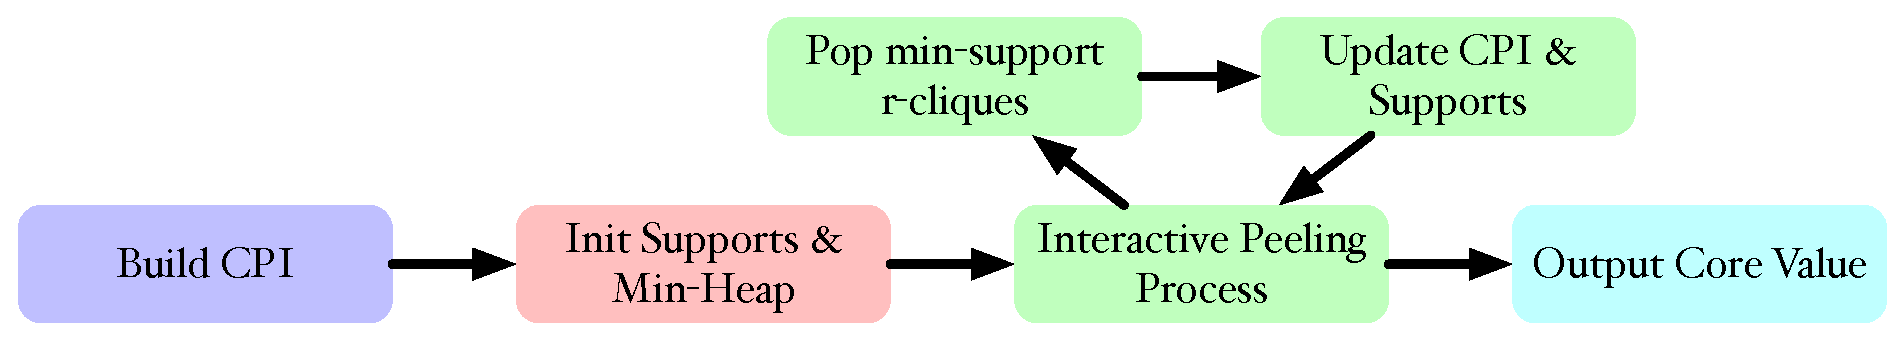
\includegraphics[width=0.45\textwidth]{figure/pipline.eps}
    % 虚线连接的节点是\pivot节点, 实线连接的节点是\hold节点.
    \caption{
        Overview of our approach.
    }
    \label{fig:pipline}
\end{figure}
}


\stitle{Index Support.}
% 上面说了4个
If an index supports these four operations efficiently, then nucleus decomposition can be performed without enumerating any $s$-cliques.
%
This removes the main bottleneck.
%
The key journal-level refinement is also simple.
%
The index is not only a compact representation of clique space.
%
It also carries the differential maintenance state used for exact support updates.
% 如果我们能找到一个索引来支持这三个操作, 那么我们就能在不枚举任何s-clique的情况下完成nuclear decomposition, 从而使算法变得不依赖于s-clique的枚举, 彻底摆脱枚举的瓶颈.


% Guided by this, we propose a minimal base framework: (i) build a CPI over $G$; (ii) compute the initial $s$-support for every $r$-clique; and (iii) peel in increasing support by repeatedly extracting the current minimum, assigning $\kappa_s(\cdot)$, removing the peeled $r$-cliques from CPI, and updating the supports of remaining neighbors along affected paths.

% To realize this framework \emph{without materializing $K_s$}, three lines in Algorithm~\ref{alg:hierarchy} require an index: line~2 (one-shot support initialization), line~11 (path-local removal of peeled $r$-cliques), and line~13 (incremental neighbor updates). Our goal is to carry out all three by \emph{counting} on CPI paths rather than \emph{enumerating} $s$-cliques.


% % \begin{algorithm}[htbp]
%     \caption{Bron-Kerbosch Algorithm}
%     \label{alg:bron_kerbosch}
%     \KwIn{Graph $G = (V, E)$}
%     \KwOut{All maximal cliques in $G$}
%     \SetKwFunction{FMain}{BronKerbosch}
%     \SetKwProg{Fn}{Function}{:}{}
%     \Fn{\FMain{$R, P, X$}}{
%         \If{$P = \emptyset \land X = \emptyset$}{
%             \Return $R$ \;
%         }
%         $u_{piv} \gets \arg\max_{x\in P} |P\cap N_H(x)|$ \;
%         \ForEach{$v \in P \setminus N(u_{piv})$}{
%             \FMain{$R \cup \{v\}, P \cap N(v), X \cap N(v)$} \;
%             $P \gets P \setminus \{v\}$ \;
%             $X \gets X \cup \{v\}$ \;
%         }
%     }
% \end{algorithm}

% \begin{algorithm}[htbp]
%     \caption{Bron-Kerbosch Algorithm}
%     \label{alg:bron_kerbosch}
%     \LinesNumbered
%     \KwIn{Undirected graph $G=(V,E)$}
%     \KwOut{All maximal cliques in $G$}
%     \SetKwFunction{BKMain}{BronKerbosch}
%     \SetKwProg{Fn}{Function}{:}{}

%     Compute a degeneracy ordering $(v_1,\dots,v_n)$ of $G$; let $\sigma(v_i)\leftarrow i$\;
%     Orient every edge from lower to higher rank to obtain $N^{+}(\cdot)$;
    
%     \ForEach{$v \in V$ in increasing order of $\sigma$}{
%         $P \gets N^{+}(v)$,\quad $X \gets N(v)\setminus N^{+}(v)$\;
%         \BKMain{$\{v\},\; P,\; X$}\;
%     }

%     \Fn{\BKMain{$R, P, X$}}{
%         \If{$P=\emptyset \land X=\emptyset$}{
%             \textbf{output clique }$R$\;
%             \Return
%         }
%         $u_{\text{piv}} \gets \arg\max_{x \in P \cup X} |\,P \cap N(x)\,|$ 
        
%         \ForEach{$v \in P \setminus N(u_{\text{piv}})$}{
%             \BKMain{$R \cup \{v\},\; P \cap N(v),\; X \cap N(v)$}\;
%             $P \gets P \setminus \{v\}$\;
%             $X \gets X \cup \{v\}$\;
%         }
%     }
    
    
% \end{algorithm}

% \begin{algorithm}[htbp]
%     \caption{Bron-Kerbosch Algorithm}
%     \label{alg:bron_kerbosch}
%     \KwIn{Graph $G=(V,E)$}
%     \KwOut{All maximal cliques in $G$ (each reported once)}
%     \SetKwFunction{BKMain}{BronKerbosch}
%     \SetKwProg{Fn}{Function}{:}{}

%     Compute a degeneracy ordering $(v_1,\dots,v_n)$ of $G$  
%     Orient every edge from lower to higher rank to obtain $N^{+}(\cdot)$\;

%     \ForEach{$v \in V$ in increasing order of $\sigma$}{
%         $P \gets N^{+}(v)$\;
%         \BKMain{$\{v\}, P$}\;
%     }

%     \Fn{\BKMain{$R, P$}}{
%         \If{$P=\emptyset$}{
%             \Return $R$ 
%         }
%         $u_{\text{piv}} \gets \arg\max_{x\in P} |P \cap N(x)|$ 

%         \ForEach{$v \in P \setminus N(u_{\text{piv}})$}{
%             \BKMain{$R \cup \{v\},\;\; P \cap N(v)$}\;
%             $P \gets P \setminus \{v\}$ 
%         }
%     }
    
% \end{algorithm}




% \begin{algorithm}[t!]
%     \caption{\textsc{Build--SCT}$(G,\,s)$}
%     \label{alg:buildSCT}
%     \KwIn{Undirected graph $G=(V,E)$, optional size cap $s$}
%     \KwOut{Succinct Clique Tree of $G$}

%     Compute a degeneracy ordering $(v_1,\dots,v_n)$ of $G$  
%     Orient every edge from lower to higher rank to obtain $N^{+}(\cdot)$\;

%     \For(\tcp*[f]{one root per vertex}){$i\gets 1$ \KwTo $n$}{
%         $V_{Hold}\gets\{v_i\}$ $P\gets N^{+}(v_i)$ $V_{Pivot}\gets\emptyset$

%         \textsc{ExpandPath}$(P, V_{Hold}, V_{Pivot})$\;
%     }

%     \SetKwFunction{Expand}{ExpandPath}
%     \SetKwProg{Fn}{Function}{:}{}

%     \Fn{\Expand{$P, V_{Hold}, V_{Pivot}$}}{
%         \If{$P=\emptyset$}{
%             \textbf{output path }$\{V_{Hold},\,V_{Pivot}\}$\;
%             \textbf{return}
%         }
        
%         $u_{piv} \gets \arg\max_{x\in P} |P\cap N^+(x)|$ \;
%         \For(\tcp*[f]{non-neighbors of pivot}){$v\in P\setminus N(u_{piv})$}{
%             $P\gets P\setminus\{v\}$
            
%             \eIf{$v=u_{piv}$}{
%                 \Expand{$P\cap N(v),\;V_{Hold},\;V_{Pivot}\cup\{v\}$}
%             }{
%                 \Expand{$P\cap N(v),\;V_{Hold}\cup\{v\},\;V_{Pivot}$}
%             }
%         }
%     }
% \end{algorithm}

% Lemma 4.6 (Path pruning). Let P be a path in the CPI and let
% 𝑠 ≥ 1 be the target clique size. Then P encodes at least one 𝑠-clique iff
% |𝑉ℎ (P)| ≤ 𝑠 ≤ |𝑉ℎ (P)| + |𝑉𝑝 (P)| .
% Equivalently, P can be safely pruned for size 𝑠 iff
% 𝑠 < |𝑉ℎ (P)| or 𝑠 > |𝑉ℎ (P)| + |𝑉𝑝 (P)| .
% Example 4.7. Considering the CPI shown in Figure 3, if we need

\begin{algorithm}[t!]
    \caption{\textsc{Build--CPI}$(G,\,s)$}
    \label{alg:buildCPI}
    \KwIn{Undirected graph $G=(V,E)$, optional size cap $s$}
    \KwOut{Clique Path Index (CPI) of $G$}

    Compute a degeneracy ordering $(v_1,\dots,v_n)$ of $G$  
    Orient every edge from lower to higher rank to obtain $N^{+}(\cdot)$\;

    \For(\tcp*[f]{one root per vertex}){$i\gets 1$ \KwTo $n$}{
        $V_{Hold}\gets\{v_i\}$ $P\gets N^{+}(v_i)$ $V_{Pivot}\gets\emptyset$

        \textsc{ExpandPath}$(P, V_{Hold}, V_{Pivot})$\;
    }

    \SetKwFunction{Expand}{ExpandPath}
    \SetKwProg{Fn}{Function}{:}{}

    \Fn{\Expand{$P, V_{Hold}, V_{Pivot}$}}{

    % path pruning
        \lIf{$|V_{Hold}| > s$}{
            \textbf{return}
        }

        \If{$P=\emptyset$}{
            %  \textbf{or} $|V_{Hold}| + |V_{Pivot}| < s
            % \textbf{output path }$\{V_{Hold},\,V_{Pivot}\}$\;
            % \textbf{return}
            \If{$|V_{Hold}| + |V_{Pivot}| \ge s$}{
                \textbf{output path }$\{V_{Hold},\,V_{Pivot}\}$\;
            }
            \textbf{return}
        }
        
        $u_{piv} \gets \arg\max_{x\in P} |P\cap N^+(x)|$ \;
        \For(\tcp*[f]{non-neighbors of pivot}){$v\in P\setminus N(u_{piv})$}{
            $P\gets P\setminus\{v\}$
            
            \eIf{$v=u_{piv}$}{
                \Expand{$P\cap N(v),\;V_{Hold},\;V_{Pivot}\cup\{v\}$}
            }{
                \Expand{$P\cap N(v),\;V_{Hold}\cup\{v\},\;V_{Pivot}$}
            }
        }
    }
\end{algorithm}

\subsection{Succinct Clique Tree} \label{sec:sct}

% \noindent\textit{Motivation from our base framework.}
% In the base framework (Algorithm~\ref{alg:hierarchy}, CND), three operations require an index that avoids materializing $K_s$: the one-shot initialization of $(r,s)$-supports (line 2), the path-local removal of peeled $r$-cliques (line 11), and the incremental update of neighbors' supports (line 13). Since the final output does not need to list any $s$-clique, we seek a counting representation rather than an enumeration of $K_s$.

% \noindent Succinct Clique Tree (SCT)\cite{Pivoter} is a Bron-Kerbosch-inspired representation that organizes the pivoting search space for exact clique counting.
% 
% \textit{Construction and stored semantics.} Using% \begin{definition}[clique path]
% \label{def:root_leaf_path}
% Given a \emph{Succinct Clique Tree}, a \emph{clique path}
% is a path that starts from the root node and ends at a leaf node, denoted as $\TPath{}$.
% All clique paths are enumerated in a \textbf{left-to-right
% depth-first search (DFS) order}.  We denote the $i$-th path in this
% DFS order by $\TPath{i}$.
%
% Formally, let
% \[
%   \TPath{i} = \langle v_{a_1}, v_{a_2}, \dots, v_{a_\ell} \rangle ,
% \]
% where $v_{a_1}$ is the root, $v_{a_\ell}$ is the corresponding leaf,
% and $\ell$ is the length of the path.  The index $i$ reflects the
% position of this path in the DFS enumeration described above.
% \end{definition}
%
% \begin{example}
% \label{ex:sct_example}
% Figure~\ref{fig:sct_example} shows an example of a Succinct Clique Tree
% (SCT). $\TPath{1} = \langle v_1, v_4, v_5, v_6 \rangle$, the second path is
% $\TPath{2} = \langle v_1, v_2, v_3, v_4, v_5 \rangle$. There are eleven
% clique paths in total, and the last path is $\TPath{11} = \langle v_8, v_9 \rangle$.
% \end{example}
%
%
% \begin{lemma}[Clique Count in a Path\cite{Pivoter}]
% \label{lem:clique_count}
% Let $\TPath{}$ be a clique path in an SCT, with
% $V_{p}(\TPath{})$ and $V_{h}(\TPath{})$ denoting its pivot
% and hold vertices, respectively.
% For any $k\ge |V_{h}(\TPath{})|$, every $k$-clique represented by
% $\TPath{}$ consists of all vertices in $V_{h}(\TPath{})$ and
% exactly $k-|V_{h}(\TPath{})|$ vertices chosen from $V_{p}(\TPath{})$.
% Hence $\#\text{$k$-cliques on }\TPath{}$ is equal to $ \binom{|V_{p}(\TPath{})|}{\,k-|V_{h}(\TPath{})|\,}.$
% \end{lemma}
%
% \begin{example}
%   For SCT as shown in Figure~\ref{fig:sct_example}.
%   $V_{p}(\TPath{1}) = \{v_4, v_5\}$ and
%   $V_{h}(\TPath{1}) = \{v_1,v_6\}$. Thus, the number of $3$-cliques on $\TPath{1}$ is equal to $ \binom{2}{\,3-2\,} = 2.$ $V_{p}(\TPath{2}) = \{v_2, v_3, v_4, v_5\}$ and $V_{h}(\TPath{2}) = \{v_1\}$. Thus, the number of $3$-cliques on $\TPath{2}$ is equal to $ \binom{4}{\,3-1\,} = 6.$
% \end{example} a degeneracy ordering, we orient edges from lower to higher rank to obtain $N^+(\cdot)$. For each vertex $v$ (in order), SCT starts a root with \emph{hold} set $V_h{=}\{v\}$ and \emph{pivot} set $V_p{=}N^+(v)$ and recursively expands by pivoting: choose a pivot $u\in V_p$ (e.g., maximizing $|V_p\cap N^+(u)|$) and branch only on $V_p\setminus N(u)$ while shrinking candidates to $V_p\cap N(\cdot)$. Each state stores exactly two sets—$V_h$ (already fixed) and $V_p$ (eligible extensions); along any path, $V_h$ are mandatory and $V_p$ are selectable, so a path summarizes a family of cliques without enumerating them one by one.

% \noindent\textit{SOTA counting in brief.}
% To efficiently count cliques without explicit enumeration, we first review the state-of-the-art clique counting method, the \textit{Succinct Clique Tree (\sct)}~\cite{Pivoter}. 
% \sct compacts the Bron--Kerbosch pivoting search space for exact clique counting. Vertices are processed in degeneracy order and edges are oriented to define $N^+(\cdot)$. For each root $v$, every state stores two sets—$V_h$ (hold, already fixed) and $V_p$ (pivot, eligible extensions). Pivoting on $u\in V_p$ branches only on $V_p\setminus N(u)$ while shrinking candidates to $V_p\cap N(\cdot)$. Thus each clique path succinctly summarizes a family of cliques without enumerating them.
We first review the state-of-the-art clique counting method, the \textit{Succinct Clique Tree} (\sct)~\cite{Pivoter}. 
The \sct compacts the Bron--Kerbosch pivoting search space for exact clique counting. 
Instead of enumerating all cliques, \sct constructs a hierarchical search tree in which each node corresponds to a state in the Bron--Kerbosch maximal clique search (the pivot-based version)~\cite{BronKerbosch,bitsetClique}, thereby implicitly representing all subcliques. 
Vertices are processed in \textit{degeneracy order}, and edges are oriented to define $N^+(\cdot)$. 
For each root vertex $v$ in \sct, every state maintains two sets: $V_h$ (\hold, already fixed) and $V_p$ (\pivot, eligible extensions). 
Pivoting on $u \in V_p$ branches only on $V_p \setminus N(u)$ while restricting candidates to $V_p \cap N(\cdot)$. 
Thus, each \textit{clique} path succinctly represents a family of cliques without enumerating them explicitly. 
This structure supports aggregated counting of all subcliques (of sizes $r$, $s$, etc.), enabling exact clique counting without enumeration.


% \begin{algorithm}[t]
\small
% \caption{UpdateSupport}
% \label{alg:updateSupport}
% % $R_{min}$, $I$, $support$, $H_{\min}$)
% \KwIn{$r$-cliques $R_{min}$ removed, \sct $I$, support map $support$, min heap $H_{\min}$}
% \KwOut{Updated support map $support$ and min heap $H_{\min}$}
% \SetKwFunction{UpdateIndex}{UpdateIndex}
% \SetKwProg{Fn}{Function}{:}{}

% \ForEach{path $\TPath$ in $I$ that intersects any $rc \in R_{min}$}{
%     \ForEach{$rc covered$ by $\TPath$}{
%         old$\gets support(rc)$\;
%         recompute $support(rc)$ based on $\TPath$\;
%         \If{support(rc) changed}{
%             update $H_{\min}$ with new support value\;
%         }
%     }
% }
% \end{algorithm}

% 
% Bron-Kerbosch\cite{BronKerbosch}是枚举极大团的经典算法, 其通过对三个顶点集合$R$, $P$, $X$的递归回溯来枚举所有极大团. 其中$R$表示当前已经找到的极大团, $P$表示当前可能的顶点集合, $X$表示已经被排除的顶点集合. 该算法的时间复杂度为$O(3^{n/3})$, 其中$n$是图中顶点的个数.
% \paragraph{Bron--Kerbosch enumeration framework.}

% During each recursive call it keeps three pairwise-disjoint vertex sets, 
% $R$ denotes the current (partial) clique,
% $P$ comprises those vertices that may still be added to extend $R$,
% and $X$ collects vertices that have already been explored and must therefore be excluded.
% Given a vertex $v\in P$, the algorithm moves $v$ into $R$, updates
% $P\leftarrow P\cap N(v)$ and $X\leftarrow X\cap N(v)$, and then recurses.
% When both $P$ and $X$ become empty, $R$ constitutes a maximal clique.
% 首先先把图中的定点按照退化序进行排序,随后按照退化许序进行枚举. 每次只关注ordering中比当前顶点大的邻居, 这样可以避免重复枚举.
% 随后在\BKMain中, 如果$P$为空, 则说明当前的$R$是一个极大团, 将其输出. 否则选择一个枢纽顶点$u_{piv}$, 只对$P\setminus N(u_{piv})$中的顶点进行递归. 这样可以大大减少递归的分支数.
% At line 1, the algorithm first computes a degeneracy ordering of the graph and orients every edge from lower to higher rank to obtain $N^{+}(\cdot)$. Then, it iterates over each vertex $v$ in increasing order of the degeneracy ordering $\sigma$ at line 3. For each vertex $v$, it initializes the candidate set $P$ to $N^{+}(v)$ and calls the recursive function \BKMain with the current clique $R$ initialized to $\{v\}$ and the candidate set $P$ at line 4.

% In the recursive function \BKMain, if the candidate set $P$ is empty, it indicates that the current clique $R$ is maximal, and it is output at line 7. Otherwise, a pivot vertex $u_{\text{piv}}$ is selected at line 9, and the algorithm recurses only on the vertices in $P\setminus N(u_{\text{piv}})$ at line 11. This strategy significantly reduces the number of recursive branches.

% \begin{figure*}[htbp]
%     \centering
%     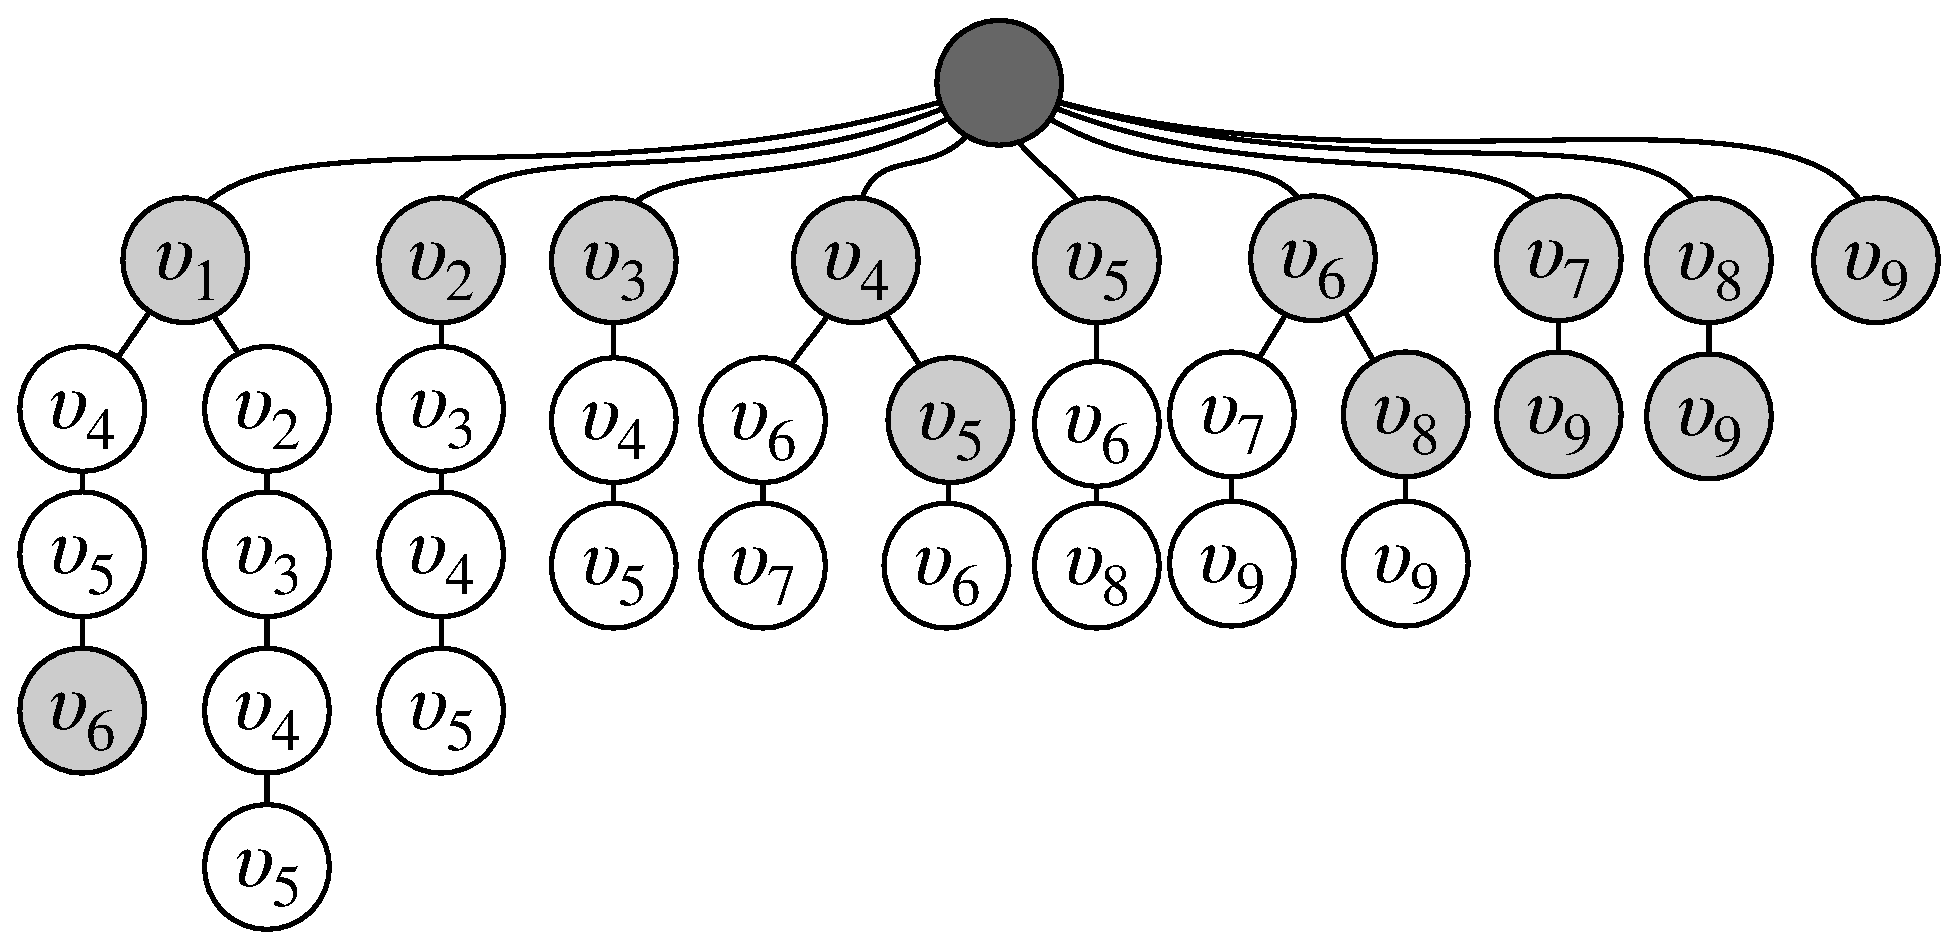
\includegraphics[width=0.9\textwidth]{figure/tree.eps}
%     \caption{An example of a Succinct Clique Tree (SCT). The white nodes represent pivots.}
%     \label{fig:sct_example}
% \end{figure*}
\begin{figure}[tb]
    \centering
    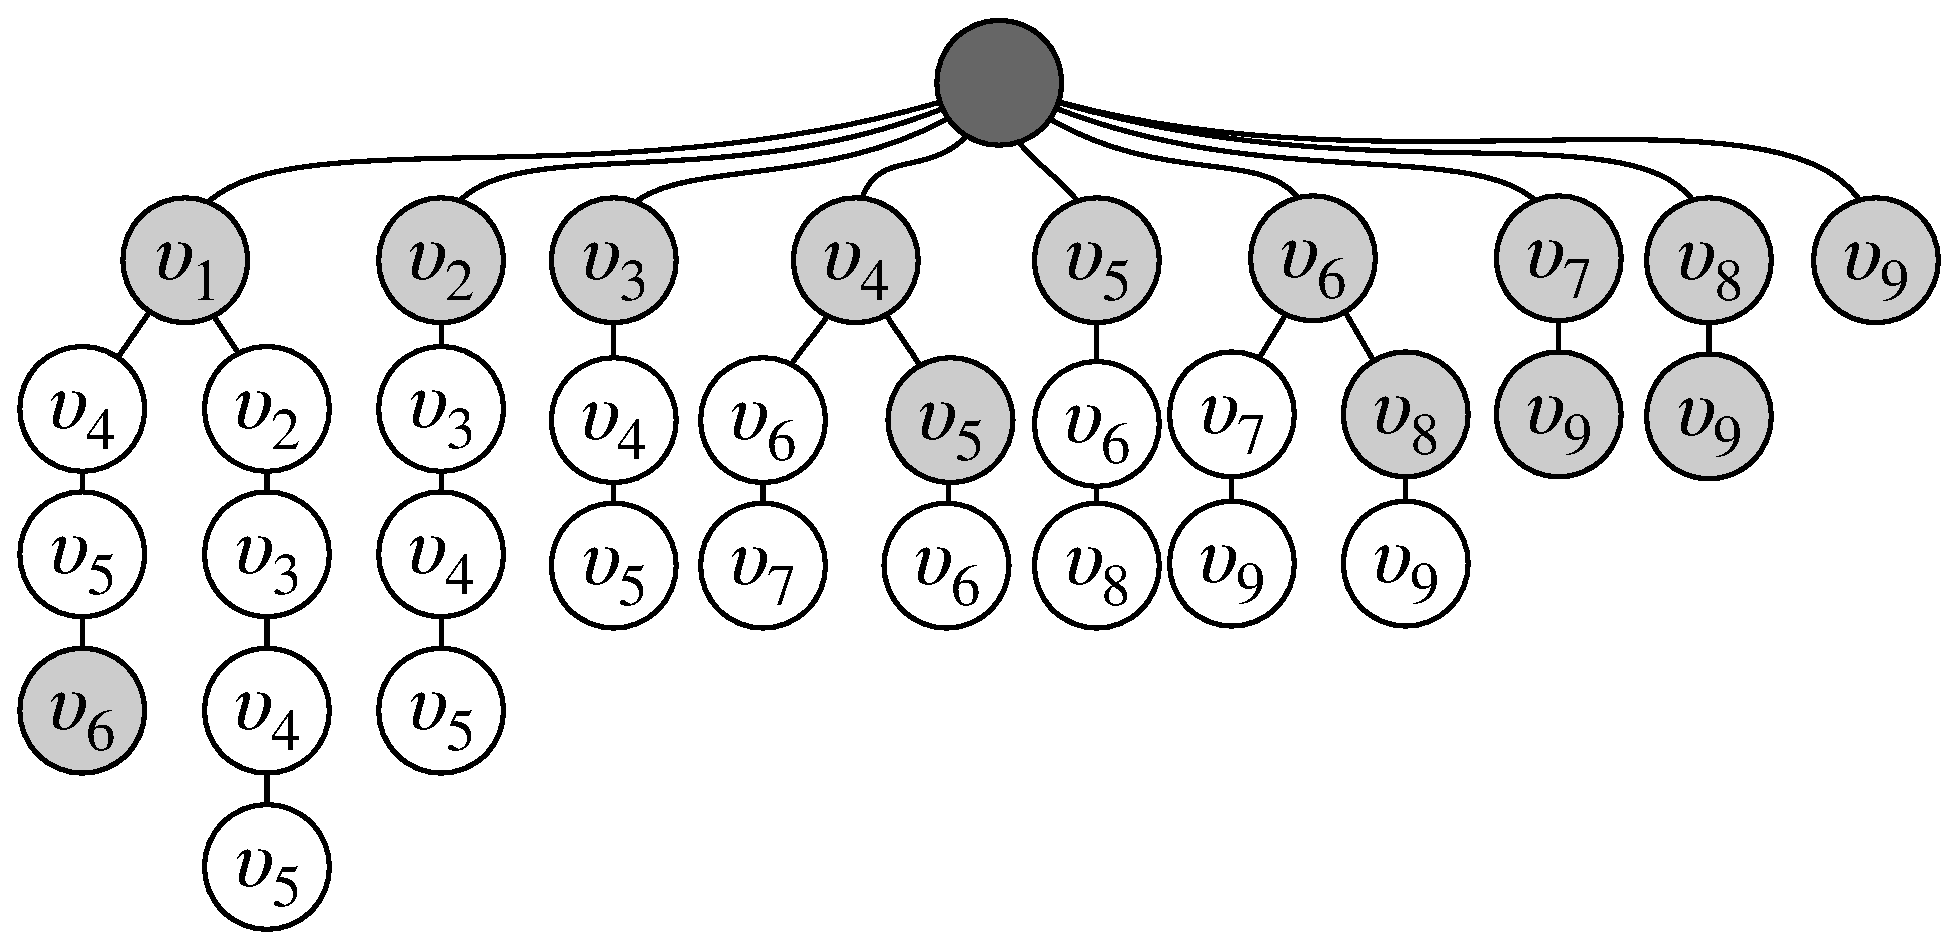
\includegraphics[width=0.43\textwidth]{figure/tree.eps}
    \caption{An example of a Succinct Clique Tree (\sct). White nodes denote pivots; gray nodes denote holds.}
    \label{fig:sct_example}
\end{figure}

% 基于出名的Bron-Kerbosch的理论, \cite{Pivoter}对此进行了一些改进, 提出了一个基于压缩的Succinct Clique Tree (SCT)的表示方法. 他们删除了$X$集合, 只保留$R$和$P$两个集合, 如Algorithm~\ref{alg:buildSCT}所示.
% The Bron--Kerbosch algorithm\cite{BronKerbosch,bitsetClique} is a seminal backtracking scheme for enumerating maximal cliques. Building on the same pivoting-style search space, Pivoter\cite{Pivoter} introduced the Succinct Clique Tree (SCT), which organizes the recursion into a compact multiway structure. Each state carries two sets: a \emph{hold} set $V_h$ (vertices already selected) and a \emph{pivot} set $V_p$ (eligible extensions), compactly capturing families of cliques. Figure~\ref{fig:sct_example} shows the SCT constructed for the example graph in Figure~\ref{fig:graph_example}.

% The Bron-Kerbosch algorithm\cite{BronKerbosch,bitsetClique} is a seminal back-tracking scheme for enumerating all maximal cliques in an undirected graph. 
% Based on the Bron-Kerbosch algorithm, \cite{Pivoter} introduced a Succinct Clique Tree (SCT) representation method that compresses the search space, as shown in Algorithm~\ref{alg:buildSCT}. The algorithm ultimately generates a multi-way tree, where each clique path represents a clique.
Figure~\ref{fig:sct_example} illustrates the SCT constructed for the example graph shown in Figure~\ref{fig:graph_example}.
% 为了方便后续介绍, 我们定义了根到叶子的路径, 如下所示:
We first define a \textit{clique path} as follows: 


\begin{definition}[Clique Path]\label{def:root_leaf_path}
In a Succinct Clique Tree, a \emph{clique path} $\TPath{}$ is any root-to-leaf path.  
All clique paths are enumerated in left-to-right depth-first order, with the $i$-th path denoted by $\TPath{i}$.
Formally,
$
  \TPath{i} = \langle v_{a_1}, v_{a_2}, \dots, v_{a_\ell} \rangle,
$
where $v_{a_1}$ is the root, $v_{a_\ell}$ is the leaf, and $\ell$ is the path length.
\end{definition}


\begin{example}
\label{ex:sct_example}
Figure~\ref{fig:sct_example} shows an example of a \sct. $\TPath{1} = \langle v_1, v_4, v_5, v_6 \rangle$, the second path is
$\TPath{2} = \langle v_1, v_2, v_3, v_4, v_5 \rangle$. There are eleven
clique paths in total, and the last path is $\TPath{11} = \langle v_8, v_9 \rangle$.
\end{example}


% \begin{lemma}[Clique Count in a Path~\cite{Pivoter}]
\begin{lemma}[Unique Path Encoding~\cite{Pivoter}]
\label{lem:clique_count}
% Let $\TPath{}$ be a clique path in an \sct, with
% $V_{p}(\TPath{})$ and $V_{h}(\TPath{})$ denoting its pivot
% and hold vertices, respectively.
% For any $k\ge |V_{h}(\TPath{})|$, every $k$-clique represented by
% $\TPath{}$ consists of all vertices in $V_{h}(\TPath{})$ and
% exactly $k-|V_{h}(\TPath{})|$ vertices chosen from $V_{p}(\TPath{})$.
% Hence $\#\text{$k$-cliques on }\TPath{}$ is equal to $ \binom{|V_{p}(\TPath{})|}{\,k-|V_{h}(\TPath{})|\,}.$

% 对于图中任何的$k$-clique $C_k$, 都存在且仅存在一个根到叶子的路径$\TPath{} = V_h(\TPath{}) \cup V_p(\TPath{})$满足$V_h(\TPath{}) \subseteq C_k \subseteq V_h(\TPath{}) \cup V_p(\TPath{})$. 其中$V_h(\TPath{})$和$V_p(\TPath{})$分别表示路径$\TPath{}$上的hold顶点和pivot顶点集合.
For any $k$-clique $C_k$ in the graph, there exists only one clique path $\TPath{} = V_h(\TPath{}) \cup V_p(\TPath{})$ such that $V_h(\TPath{}) \subseteq C_k \subseteq (V_h(\TPath{}) \cup V_p(\TPath{}))$. Here, $V_h(\TPath{})$ and $V_p(\TPath{})$ denote the sets of hold vertices and pivot vertices on the path $\TPath{}$, respectively.
\end{lemma}

Intuitively, any $k$-clique represented by a path $\TPath$ must include all hold vertices of that path, while the pivot vertices are optional. 
%
Formally, a $k$-clique $C_k$ is \emph{encoded} by a \cpi\ path $\TPath$ if and only if $V_h(\TPath) \subseteq C_k \subseteq V_h(\TPath) \cup V_p(\TPath)$; 
it is \emph{covered} by $\TPath$ if and only if  $C_k \subseteq V_h(\TPath) \cup V_p(\TPath)$.


\begin{example}
  For \sct as shown in Figure~\ref{fig:sct_example}.
  $V_{p}(\TPath{1}) = \{v_4, v_5\}$ and
  $V_{h}(\TPath{1}) = \{v_1,v_6\}$. Thus, the number of $3$-cliques on $\TPath{1}$ is equal to $ \binom{2}{\,3-2\,} = 2.$ $V_{p}(\TPath{2}) = \{v_2, v_3, v_4, v_5\}$ and $V_{h}(\TPath{2}) = \{v_1\}$. Thus, the number of $3$-cliques on $\TPath{2}$ is equal to $ \binom{4}{\,3-1\,} = 6.$
\end{example}

% \noindent\textit{Scope.}

\stitle{Inadequacies in \sct Structures.} 
\sct is designed solely for clique counting on static graphs. 
For the key functions in our framework (Algorithm~\ref{alg:framework}), 
\sct can support \textsc{$s$-CliqueCount} (i.e., initializing the support) with minor modifications. 
However, it lacks dynamic update capabilities and cannot be trivially extended to support \textsc{UpdateIndex} and \textsc{UpdateSupport}, which are required in our representation layer to remove peeled $r$-cliques efficiently. 
%
This limitation motivates the design of a new index that can support all these operations, which is both non-trivial and challenging.


% our Clique Path Index (\cpi) in next subsection, which adapts SCT to support efficient batched updates.
% a static counting structure: it directly supports 
% line~2 (one-shot initialization of $(r,s)$-supports) 
% but does not provide the dynamic path-local updates required by line~9 (removing peeled $r$-cliques from the index) and line~10 (updating neighbors' supports). 
% This limitation motivates our Clique Path Index (\cpi) in next subsection, which adapts SCT to support efficient batched updates.


% (i) \textsc{$s$-CliqueCount}, which initializes the $s$-support for each $r$-clique (Line~2); 
% (ii) \textsc{UpdateIndex}, which removes peeled $r$-cliques (Line~9); and 
% (iii) \textsc{UpdateSupport}, which identifies and updates the supports of affected $r$-cliques after each removal (Line~10). 

\subsection{Clique Path Index}
\label{sec:cpi}

% 在介绍我们的Derivation之前, 我们需要介绍一些基于SCT的概念和定理. 这些定理和概念是我们算法的基础.
% Before introducing our derivations, we need to present some \sct-based concepts and theorems that form the foundation of our algorithm.

% \begin{definition}[Clique path]
% \label{def:root_leaf_path}
% Given a \emph{Succinct Clique Tree}, a \emph{clique path}
% is a path that starts from the root node and ends at a leaf node, denoted as $\TPath{}$.
% All clique paths are enumerated in a \textbf{left-to-right
% depth-first search (DFS) order}.  We denote the $i$-th path in this
% DFS order by $\TPath{i}$.

% Formally, let
% \[
%   \TPath{i} = \langle v_{a_1}, v_{a_2}, \dots, v_{a_\ell} \rangle ,
% \]
% where $v_{a_1}$ is the root, $v_{a_\ell}$ is the corresponding leaf,
% and $\ell$ is the length of the path.  The index $i$ reflects the
% position of this path in the DFS enumeration described above.
% \end{definition}

% \begin{example}
% \label{ex:sct_example}
% Figure~\ref{fig:sct_example} shows an example of a Succinct Clique Tree
% (\sct). $\TPath{1} = \langle v_1, v_4, v_5, v_6 \rangle$, the second path is
% $\TPath{2} = \langle v_1, v_2, v_3, v_4, v_5 \rangle$. There are eleven
% clique paths in total, and the last path is $\TPath{11} = \langle v_8, v_9 \rangle$.
% \end{example}


% \begin{lemma}[Clique Count in a Path\cite{Pivoter}]
% \label{lem:clique_count}
% Let $\TPath{}$ be a clique path in an \sct, with
% $V_{p}(\TPath{})$ and $V_{h}(\TPath{})$ denoting its pivot
% and hold vertices, respectively.
% For any $k\ge |V_{h}(\TPath{})|$, every $k$-clique represented by
% $\TPath{}$ consists of all vertices in $V_{h}(\TPath{})$ and
% exactly $k-|V_{h}(\TPath{})|$ vertices chosen from $V_{p}(\TPath{})$.
% Hence $\#\text{$k$-cliques on }\TPath{}$ is equal to $ \binom{|V_{p}(\TPath{})|}{\,k-|V_{h}(\TPath{})|\,}.$
% \end{lemma}

% \begin{example}
%   For \sct as shown in Figure~\ref{fig:sct_example}.
%   $V_{p}(\TPath{1}) = \{v_4, v_5\}$ and
%   $V_{h}(\TPath{1}) = \{v_1,v_6\}$. Thus, the number of $3$-cliques on $\TPath{1}$ is equal to $ \binom{2}{\,3-2\,} = 2.$ $V_{p}(\TPath{2}) = \{v_2, v_3, v_4, v_5\}$ and $V_{h}(\TPath{2}) = \{v_1\}$. Thus, the number of $3$-cliques on $\TPath{2}$ is equal to $ \binom{4}{\,3-1\,} = 6.$
% \end{example}

Building on the basic idea of \sct~\cite{Pivoter}, we introduce a new data structure, the \emph{Clique Path Index} (\cpi), which is adapted to our counting-and-peeling framework and supports efficient updates.
% 
Unlike \sct, \cpi\ represents the search space as independent paths in a bipartite-like layout between vertices and paths, as illustrated in Figure~\ref{fig:new_tree_example}.
%
Thanks to this bipartite-like storage structure, we can also efficiently retrieve the paths containing each vertex and the vertices contained in each path, facilitating the implementation of the $\textsc{UpdateSupport}$ function in our framework to accurately identify affected $r$-cliques. 
% \cpi\ can be updated more efficiently than a traditional tree structure, as discussed in the next section.
Updating a traditional tree is difficult, since shared prefixes cause cascaded changes and costly subtree reattachments; accordingly, \cpi\ admits more efficient updates (details in the next section).


\begin{example}
    Figure~\ref{fig:new_tree_example} shows an example of a \cpi consisting of three paths and five vertices.
    Path 1 contains vertices $v_1,v_2,v_3,v_4,v_5$, where $v_1$ is a hold vertex and the others are pivot vertices.
    Path 2 contains vertices $v_1,v_4,v_5,v_6$, where $v_1$ and $v_6$ are hold vertices and the others are pivot vertices.
    Path 3 contains vertices $v_2,v_3,v_4,v_5$, where $v_2$ is a hold vertex and the others are pivot vertices.
\end{example}
% 

\begin{figure}[t]
  \centering
  \begin{subfigure}[t]{0.48\linewidth}
    \centering
    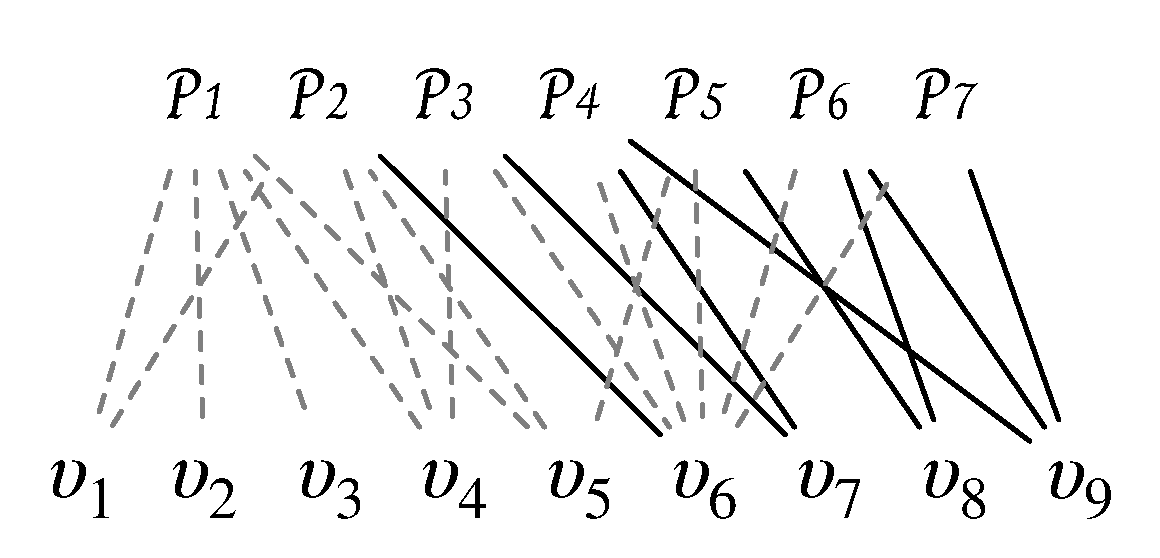
\includegraphics[width=0.8\linewidth]{figure/CPIlarge.eps}
    \caption{An example of a \cpi on Figure~\ref{fig:graph_example} (no pruning).}
    \label{fig:new_tree_example}
  \end{subfigure}
  \hspace{0.01\linewidth}
  \begin{subfigure}[t]{0.48\linewidth}
    \centering
    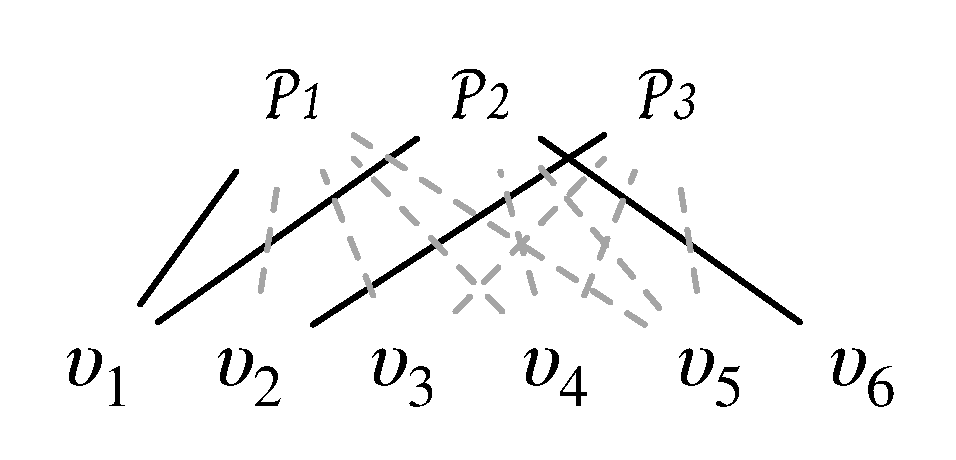
\includegraphics[width=0.8\linewidth]{figure/pruningTree.eps}
    \caption{An example of a pruned \cpi\ for $s=4$ on Figure~\ref{fig:sct_example}.}
    \label{fig:pruning_example}
  \end{subfigure}

  \caption{Examples of \cpi\ before and after pruning. Dashed nodes denote pivots, and solid nodes denote holds.}
\end{figure}

% 这种存储格式还使得我们可以高效获取到每个点所在的path以及每个path包含的点, 这使得我们可以完成我们Framework中$\textsc{UpdateSupport}$, 帮助我门来准确识别受影响的$r$-clique.
% This storage format also enables efficient retrieval of the paths containing each vertex and the vertices contained in each path, facilitating the implementation of the $\textsc{UpdateSupport}$ function in our framework to accurately identify affected $r$-cliques.



% \paragraph{Path-index storage (\cpi).}
% % 为了让tree可以高效的进行更新, 因此我们使用了二部图的方法来存储这个index, 具体来说, 我们分别存储每一条路径的hold节点和pivot节点, 如图\ref{fig:new_tree_example}所示.
% To enable efficient updates to the tree, we store the index using a bipartite-like approach. Specifically, we store the hold and pivot vertices of each path separately, 
% 该图中有

% 这里应该有\cpi的formal definition, 以及和SCT的区别.
% \todo{}


% To facilitate our discussion, We use two path-clique relations. A k-clique $C_k$ is covered by a CPI path \(\TPath\) if all its vertices lie on the path, i.e., \(C_k \subseteq V_h(\TPath)\cup V_p(\TPath)\). It is encoded by \(\TPath\) if, in addition, the path’s holds are mandatory: \(V_h(\TPath)\subseteq C_k \subseteq V_h(\TPath)\cup V_p(\TPath)\). Hence encoding implies coverage; conversely, a covered clique is encoded exactly when it contains all holds.

% To facilitate the discussion, we define that a $k$-clique $C_k$ is \emph{encoded} by a \cpi\ path $\TPath$ if and only if $V_h(\TPath) \subseteq C_k \subseteq V_h(\TPath) \cup V_p(\TPath)$. 
%
% Similarly, we define that a $k$-clique $C_k$ is \emph{covered} by a \cpi\ path $\TPath$ if and only if $C_k \subseteq V_h(\TPath) \cup V_p(\TPath)$.




% we define two types of relationships between a clique and a \cpi path based on the above theorem.

% \begin{definition}[Coverage of a $k$-clique by a path]
% \label{def:coverage_on_path}
% Let $\TPath{}$ be a CPI path with vertex set $V_h(\TPath{})\cup V_p(\TPath{})$.
% Given a $k$-clique $C_k$, we say that $C_k$ is \emph{covered} by $\TPath{}$ if and only if
% $C_k \subseteq V_h(\TPath{}) \cup V_p(\TPath{})$.
% \end{definition}


% \begin{definition}[Encoding of a $k$-clique by a path]
% \label{def:encoded_by}
% Let $\TPath{}$ be a CPI path with hold/pivot sets $V_h(\TPath{}),V_p(\TPath{})$.
% Given a $k$-clique $C_k$, we say that $C_k$ is \emph{encoded} by $\TPath{}$ if and only if
% $V_h(\TPath{}) \subseteq C_k \subseteq V_h(\TPath{}) \cup V_p(\TPath{})$.
% \end{definition}



Based on Lemma~\ref{lem:clique_count}, we derive Lemma~\ref{lem:s_support_r}, which enables the computation of the number of $s$-cliques for each $r$-clique without enumerating any $s$-cliques.

\begin{lemma}[Local $s$-support of an $r$-clique]
\label{lem:s_support_r}
Let $\TPath{}$ be a path in the \cpi with
pivot set $V_{p}$ and hold set $V_{h}$
$(h=|V_{h}|,\;p=|V_{p}|)$,
and fix integers $0<r<s$.
For any $r$-clique $C_r\subseteq\TPath{}$ set
$b \;=\; |\,C_r\cap V_{p}\,|,$
Then the number of distinct $s$-cliques on $\TPath{}$ that contain
$C_r$ equals
$
\#_{s}(C_r)
\;=\;
\binom{p-b}{\,s-h-b}.
$
\end{lemma}

\begin{proof}
Every $s$-clique on the path is
$V_h\cup Q$ with $Q\subseteq V_p$ and $|Q|=s-h$
(Lemma \ref{lem:clique_count}).
Fix any $r$-clique $C_r$ and let $b=|C_r\cap V_p|$.
Since $C_r$ already contributes those $b$ pivots,
an $s$-clique containing $C_r$ is obtained precisely by choosing the
remaining $s-h-b$ pivots from the $p-b$ unused pivots in $V_p$.
The number of such choices is
$\binom{p-b}{\,s-h-b}$,
which is zero whenever the lower or upper bound is violated.
\end{proof}
% 基于Lemma~\ref{lem:clique_count}, 我们可以在不枚举任何$s$-clique的情况下计算每个$r$-clique的$s$-clique的个数.同时考虑到我们只需要考虑$s$-clique的数量, 我们可以对SCT进行一些优化, 忽视掉那些不包含$r$-clique的路径.
% Based on Lemma~\ref{lem:clique_count}, we can compute the number of $s$-cliques for each $r$-clique without enumerating any $s$-cliques, as shown in Algorithm~\ref{alg:local_s_clique_count}. 

% 
% 基于Lemma~\ref{lem:s_support_r}, 我们推出了算法~\ref{alg:local_s_clique_count}. 来计算每个$r$-clique的$s$-clique的个数.
% \Fn{CountPreClique}{
%     \KwIn{SCT $\tree$, Clique size $r$, Clique size $s$}
%     \KwOut{$s$-clique count for every $r$-clique in $\tree$}
%     initialise $count(C_r)\leftarrow 0$ for all $r$-cliques in $\tree$\;
%     \ForEach{clique path $\TPath{}$ in $\tree$}{
%         \ForEach{$r$-clique $C_r$ in $\TPath{}$}{
%             % let $P$ be the set of pivots and $H$ be the set of holds along $\TPath{}$\;
%             $V_{p}\gets \{v \in \TPath{} \mid v \text{ is a pivot}\}$;

%             $V_{h}\gets \{v \in \TPath{} \mid v \text{ is a hold}\}$

%             $need\gets s-|V_{h}|$\;
%             $count(C_r)\gets count(C_r)+\binom{|V_{p}|}{need}$ for every $C_r\in \TPath{}$\;
%         }
%     }

%     \Return $count(C_r)$ for all $r$-cliques in $\tree$; 
% }

\begin{algorithm}[t]
\small
\caption{\textsc{$s$-CliqueCount}}
\label{alg:local_s_clique_count}
\KwIn{Clique Path Index $\tree$, clique sizes $0<r<s$}
\KwOut{$count(C_r)$ for every $r$-clique $C_r\subseteq G$}

\BlankLine
initialise $count(C_r)\gets 0$ for all $r$-cliques in $\tree$\;

\ForEach{clique path $\TPath{}$ in $\tree$}{
    $V_{h}\gets\{v\in\TPath{}\mid v\text{ is hold}\}$\;
    $V_{p}\gets\{v\in\TPath{}\mid v\text{ is pivot}\}$\;

    \ForEach{$r$-set $C_r\subseteq \TPath$}{
        $b\gets |C_r\cap V_{p}|$  

        $count(C_r)\mathrel{+}= \binom{|V_{p}|-b}{\,s-|V_{h}|-b}$\;
    }
}

\Return{$count(C_r)$ for all $r$-cliques $C_r$}\;
\end{algorithm}
Based on Lemma~\ref{lem:s_support_r}, we derive Algorithm~\ref{alg:local_s_clique_count} to compute the number of $s$-cliques for each $r$-clique without explicit enumeration.

% 为了加快tree的构建以及减小tree的存储, 我们发现了了以下pruning的规则.
\stitle{Path Pruning.} 
Naively building the index would include information about all cliques in the graph. 
However, in $(r,s)$-nucleus decomposition, not all cliques are necessary—we are only interested in cliques that contains $s$-cliques. 
To accelerate index construction and reduce its size, we introduce the following pruning rule.



% To facilitate our discussion, we define two types of relationships between a clique and a \cpi path based on the above theorem.


% 在构建过程中, 如果$hold$节点的个数大于$r$-clique的个数, 则该路径不包含任何$r$-clique, 因此可以忽略掉该路径.
% 如果该条路径的节点数量小于$r$-clique的个数, 则该路径也不包含任何$r$-clique, 因此也可以忽略掉该路径.

% 我们通过以下的引理来证明了使用SCT是会比存储或者遍历$s$-clique更加高效.
\begin{lemma}[Feasibility of Path]\label{lem:path_pruning}
Let $\TPath{}$ be a path in the \cpi and let $s\ge 1$ be the target clique size.
Then $\TPath{}$ encodes at least one $s$-clique iff
$
   |V_h(\TPath{})| \;\le\; s \;\le\; |V_h(\TPath{})| + |V_p(\TPath{})|\,.
$
\end{lemma}

\begin{proof}
  % 根据Lemma ~\ref{lem:clique_count}, 我们知道, $\TPath{}$上所有的$s$-clique都是由$V_h(\TPath{})$和$V_p(\TPath{})$组成的. 因此, 如果$s < |V_h(\TPath{})|$, 则不可能存在一个$s$-clique包含所有的hold节点, 因此不存在任何的$s$-clique. 同理, 如果$s > |V_h(\TPath{})| + |V_p(\TPath{})|$, 则不可能存在一个$s$-clique包含所有的hold节点和足够数量的pivot节点, 因此也不存在任何的$s$-clique.
  ($\Rightarrow$)According to Lemma ~\ref{lem:clique_count}, all $s$-cliques on $\TPath{}$ consist of vertices from $V_h(\TPath{})$ and $V_p(\TPath{})$. 
  Therefore, if $s < |V_h(\TPath{})|$, it is impossible for any $s$-clique to include all hold vertices, and thus no $s$-clique exists. 
  Similarly, if $s > |V_h(\TPath{})| + |V_p(\TPath{})|$, it is impossible for any $s$-clique to include all hold vertices and enough pivot vertices, and thus no $s$-clique exists.
  % 反之, 如果$s$在这个区间内, 则我们可以根据Lemma ~\ref{lem:clique_count}构造出至少一个$s$-clique, 因此存在至少一个$s$-clique.
  ($\Leftarrow$)Conversely, if $s$ lies within this interval, we can construct at least one $s$-clique based on Lemma ~\ref{lem:clique_count}, ensuring the existence of at least one $s$-clique. 
\end{proof}

% \begin{lemma}[Path pruning]\label{lem:path_pruning}
% Let $\TPath{}$ be a path in the \cpi and let $s\ge 1$ be the target clique size.
% Then $\TPath{}$ can be safely pruned for size $s$ iff
% \[
%    s < |V_h(\TPath{})|\quad\text{or}\quad s > |V_h(\TPath{})| + |V_p(\TPath{})|\,.
% \]
% \end{lemma}

% \begin{proof}
% Immediate from Lemma~\ref{lem:path_feasible} by negating the feasibility interval.
% \end{proof}

\begin{example}
  % 对于由图\ref{fig:sct_example}所展示的SCT, 如果我们需要计算4-clique的counting, 那么我们就可以将此SCT删除为只保留三个Path, 分别是
  Considering the \cpi shown in Figure~\ref{fig:pruning_example}, if we need to count $4$-cliques, we can prune this \cpi to retain only three paths, as illustrated in Figure~\ref{fig:pruning_example}. Compared to the \sct(Figure \ref{fig:sct_example}), the pruned \cpi has fewer paths, making it more efficient to store and traverse.
\end{example}

% \begin{algorithm}[htbp]
%     \caption{Bron-Kerbosch Algorithm}
%     \label{alg:bron_kerbosch}
%     \KwIn{Graph $G = (V, E)$}
%     \KwOut{All maximal cliques in $G$}
%     \SetKwFunction{FMain}{BronKerbosch}
%     \SetKwProg{Fn}{Function}{:}{}
%     \Fn{\FMain{$R, P, X$}}{
%         \If{$P = \emptyset \land X = \emptyset$}{
%             \Return $R$ \;
%         }
%         $u_{piv} \gets \arg\max_{x\in P} |P\cap N_H(x)|$ \;
%         \ForEach{$v \in P \setminus N(u_{piv})$}{
%             \FMain{$R \cup \{v\}, P \cap N(v), X \cap N(v)$} \;
%             $P \gets P \setminus \{v\}$ \;
%             $X \gets X \cup \{v\}$ \;
%         }
%     }
% \end{algorithm}

% \begin{algorithm}[htbp]
%     \caption{Bron-Kerbosch Algorithm}
%     \label{alg:bron_kerbosch}
%     \LinesNumbered
%     \KwIn{Undirected graph $G=(V,E)$}
%     \KwOut{All maximal cliques in $G$}
%     \SetKwFunction{BKMain}{BronKerbosch}
%     \SetKwProg{Fn}{Function}{:}{}

%     Compute a degeneracy ordering $(v_1,\dots,v_n)$ of $G$; let $\sigma(v_i)\leftarrow i$\;
%     Orient every edge from lower to higher rank to obtain $N^{+}(\cdot)$;
    
%     \ForEach{$v \in V$ in increasing order of $\sigma$}{
%         $P \gets N^{+}(v)$,\quad $X \gets N(v)\setminus N^{+}(v)$\;
%         \BKMain{$\{v\},\; P,\; X$}\;
%     }

%     \Fn{\BKMain{$R, P, X$}}{
%         \If{$P=\emptyset \land X=\emptyset$}{
%             \textbf{output clique }$R$\;
%             \Return
%         }
%         $u_{\text{piv}} \gets \arg\max_{x \in P \cup X} |\,P \cap N(x)\,|$ 
        
%         \ForEach{$v \in P \setminus N(u_{\text{piv}})$}{
%             \BKMain{$R \cup \{v\},\; P \cap N(v),\; X \cap N(v)$}\;
%             $P \gets P \setminus \{v\}$\;
%             $X \gets X \cup \{v\}$\;
%         }
%     }
    
    
% \end{algorithm}

% \begin{algorithm}[htbp]
%     \caption{Bron-Kerbosch Algorithm}
%     \label{alg:bron_kerbosch}
%     \KwIn{Graph $G=(V,E)$}
%     \KwOut{All maximal cliques in $G$ (each reported once)}
%     \SetKwFunction{BKMain}{BronKerbosch}
%     \SetKwProg{Fn}{Function}{:}{}

%     Compute a degeneracy ordering $(v_1,\dots,v_n)$ of $G$  
%     Orient every edge from lower to higher rank to obtain $N^{+}(\cdot)$\;

%     \ForEach{$v \in V$ in increasing order of $\sigma$}{
%         $P \gets N^{+}(v)$\;
%         \BKMain{$\{v\}, P$}\;
%     }

%     \Fn{\BKMain{$R, P$}}{
%         \If{$P=\emptyset$}{
%             \Return $R$ 
%         }
%         $u_{\text{piv}} \gets \arg\max_{x\in P} |P \cap N(x)|$ 

%         \ForEach{$v \in P \setminus N(u_{\text{piv}})$}{
%             \BKMain{$R \cup \{v\},\;\; P \cap N(v)$}\;
%             $P \gets P \setminus \{v\}$ 
%         }
%     }
    
% \end{algorithm}




% \begin{algorithm}[t!]
%     \caption{\textsc{Build--SCT}$(G,\,s)$}
%     \label{alg:buildSCT}
%     \KwIn{Undirected graph $G=(V,E)$, optional size cap $s$}
%     \KwOut{Succinct Clique Tree of $G$}

%     Compute a degeneracy ordering $(v_1,\dots,v_n)$ of $G$  
%     Orient every edge from lower to higher rank to obtain $N^{+}(\cdot)$\;

%     \For(\tcp*[f]{one root per vertex}){$i\gets 1$ \KwTo $n$}{
%         $V_{Hold}\gets\{v_i\}$ $P\gets N^{+}(v_i)$ $V_{Pivot}\gets\emptyset$

%         \textsc{ExpandPath}$(P, V_{Hold}, V_{Pivot})$\;
%     }

%     \SetKwFunction{Expand}{ExpandPath}
%     \SetKwProg{Fn}{Function}{:}{}

%     \Fn{\Expand{$P, V_{Hold}, V_{Pivot}$}}{
%         \If{$P=\emptyset$}{
%             \textbf{output path }$\{V_{Hold},\,V_{Pivot}\}$\;
%             \textbf{return}
%         }
        
%         $u_{piv} \gets \arg\max_{x\in P} |P\cap N^+(x)|$ \;
%         \For(\tcp*[f]{non-neighbors of pivot}){$v\in P\setminus N(u_{piv})$}{
%             $P\gets P\setminus\{v\}$
            
%             \eIf{$v=u_{piv}$}{
%                 \Expand{$P\cap N(v),\;V_{Hold},\;V_{Pivot}\cup\{v\}$}
%             }{
%                 \Expand{$P\cap N(v),\;V_{Hold}\cup\{v\},\;V_{Pivot}$}
%             }
%         }
%     }
% \end{algorithm}

% Lemma 4.6 (Path pruning). Let P be a path in the CPI and let
% 𝑠 ≥ 1 be the target clique size. Then P encodes at least one 𝑠-clique iff
% |𝑉ℎ (P)| ≤ 𝑠 ≤ |𝑉ℎ (P)| + |𝑉𝑝 (P)| .
% Equivalently, P can be safely pruned for size 𝑠 iff
% 𝑠 < |𝑉ℎ (P)| or 𝑠 > |𝑉ℎ (P)| + |𝑉𝑝 (P)| .
% Example 4.7. Considering the CPI shown in Figure 3, if we need

\begin{algorithm}[t!]
    \caption{\textsc{Build--CPI}$(G,\,s)$}
    \label{alg:buildCPI}
    \KwIn{Undirected graph $G=(V,E)$, optional size cap $s$}
    \KwOut{Clique Path Index (CPI) of $G$}

    Compute a degeneracy ordering $(v_1,\dots,v_n)$ of $G$  
    Orient every edge from lower to higher rank to obtain $N^{+}(\cdot)$\;

    \For(\tcp*[f]{one root per vertex}){$i\gets 1$ \KwTo $n$}{
        $V_{Hold}\gets\{v_i\}$ $P\gets N^{+}(v_i)$ $V_{Pivot}\gets\emptyset$

        \textsc{ExpandPath}$(P, V_{Hold}, V_{Pivot})$\;
    }

    \SetKwFunction{Expand}{ExpandPath}
    \SetKwProg{Fn}{Function}{:}{}

    \Fn{\Expand{$P, V_{Hold}, V_{Pivot}$}}{

    % path pruning
        \lIf{$|V_{Hold}| > s$}{
            \textbf{return}
        }

        \If{$P=\emptyset$}{
            %  \textbf{or} $|V_{Hold}| + |V_{Pivot}| < s
            % \textbf{output path }$\{V_{Hold},\,V_{Pivot}\}$\;
            % \textbf{return}
            \If{$|V_{Hold}| + |V_{Pivot}| \ge s$}{
                \textbf{output path }$\{V_{Hold},\,V_{Pivot}\}$\;
            }
            \textbf{return}
        }
        
        $u_{piv} \gets \arg\max_{x\in P} |P\cap N^+(x)|$ \;
        \For(\tcp*[f]{non-neighbors of pivot}){$v\in P\setminus N(u_{piv})$}{
            $P\gets P\setminus\{v\}$
            
            \eIf{$v=u_{piv}$}{
                \Expand{$P\cap N(v),\;V_{Hold},\;V_{Pivot}\cup\{v\}$}
            }{
                \Expand{$P\cap N(v),\;V_{Hold}\cup\{v\},\;V_{Pivot}$}
            }
        }
    }
\end{algorithm}
%  (Algorithm~\ref{alg:buildCPI}).
% 算法~\ref{alg:buildCPI}展示了CPI的构建方法, 该方法和SCT的构建方法较为相似, 但是不同的是每次output一整条path, 并且在构建过程中, 我们使用了Lemma~\ref{lem:path_pruning}来对路径进行剪枝.
\stitle{Index Construction.} 
Algorithm~\ref{alg:buildCPI} illustrates the construction process of \cpi. 
Contrary to \sct, \cpi outputs an entire path at once and applies Lemma~\ref{lem:path_pruning} (Line~6 $\&$ 9) to prune paths during construction.

% \stitle{Analysis.} 
Since paths in the \cpi can be pruned to retain only those that must contain $s$-cliques, we can also derive the following result.

\begin{theorem}[Number of Clique Paths]
\label{thm:path_vs_clique}
Let $\tree$ be the \cpi of a graph $G$, and let
$\mathcal P_s \;=\;
  \bigl\{\TPath{} \mid 
      |V_h(\TPath{})|\le s \text{ and } |\TPath{}|\ge s\bigr\}$
be the set of \cpi paths that remain after pruning for a given integer $s \ge 1$.
Let $\mathcal K_s$ denote the set of all $s$-cliques in $G$.
Then $|\mathcal K_s| \ge |\mathcal P_s|$.
\myaddRA{Moreover, $\sum_{P\in\mathcal P_s} |V_h(P)| \le s\,|\mathcal K_s|$.}
\end{theorem}


\begin{proof}
Let $\TPath{}$ be a path in the \cpi $\tree$.
By Lemma~\ref{lem:path_pruning}, if $\TPath{}$ survives
the pruning rule, it contains at least one $s$-clique.
Thus, every path in $\mathcal P_s$ contains at least one $s$-clique.
Therefore, the number of $s$-cliques is greater than or equal to the number of
\cpi paths in $\mathcal P_s$.
\myaddRA{By definition of $\mathcal P_s$, each $P\in\mathcal P_s$ satisfies $|V_h(P)|\le s$.
Thus $\sum_{P\in\mathcal P_s}|V_h(P)| \le s|\mathcal P_s| \le s|\mathcal K_s|$.}
\end{proof}

% 这条定理表明, 存储整个SCT的路径数目是$s$-clique的下界, 存储整个SCT一定不会比存储$s$-clique更加昂贵.
\begin{remark}
This theorem demonstrates a key advantage of our approach.
The number of paths in the \cpi\ cannot exceed the number of $s$-cliques, ensuring that storing the entire index is no more expensive than storing all $s$-cliques. 
More importantly, since each path compactly represents multiple $s$-cliques, traversing and updating the \cpi\ becomes substantially more efficient than operating on enumerated $s$-cliques. 
This property underpins the benefits of our representation layer, enabling efficient decomposition.
\end{remark}



\stitle{Complexity.}
The worst-case time to build the \cpi is $O\big(n\cdot 3^{\alpha/3}\big)$~\cite{Pivoter}, where $\alpha$ is the degeneracy of the graph, $n\cdot 3^{\alpha/3}$ is the maximum number of maximal cliques in a graph with $n$ vertices.
But in practice, due to path pruning, the actual construction time is significantly lower than this worst-case bound.
  % 
Space complexity to store CPI is $O(min(n\cdot 3^{\alpha/3}, |K_s|))$ (Theorem~\ref{thm:path_vs_clique}),
where $|K_s|$ is the number of $s$-cliques in the graph.

% 上述定义和定理为我们提供了一个强有力的工具, 来计算每个$r$-clique的$s$-clique的个数, 同时避免了枚举$s$-clique. 但是仅仅依赖SCT并不足以来进行Nuclear Core Decomposition, 如何更新在计算的过程中动态的来更新这个tree, 以及如何使用这个tree来进行Nuclear Core Decomposition, 这些都是极大的挑战. 
\stitle{From Counting to Decomposition.}
The \cpi\ provides a powerful tool for computing the number of $s$-cliques associated with each $r$-clique while avoiding explicit $s$-clique enumeration. 
%
However, efficiently updating the \cpi during computation and leveraging it to guide the decomposition process remain major technical challenges for performing nucleus core decomposition.

% 但是感谢CPI的存储结构, 这种bipartite-like存储结构, 使得我们可以以比更新Tree更加高效的方式来更新这个CPI. 我们在后续的章节中介绍了如何动态的来更新这个CPI.

% 我们首先在下一小节介绍了我们的base framework, 并且在章节\ref{sec:our_approach}中介绍了如何使用这个base framework来进行Nuclear Core Decomposition, 以及如何动态的更新这个tree.

% ---

% \paragraph{Overview.}
% A minimal \emph{base framework} built on a \textbf{Clique Path Index (CPI)} and a standard peeling routine to compute $(r,s)$-coreness.

% \paragraph{Clique Path Index (CPI).}
% A CPI path encodes a \emph{family} of cliques. We denote a path by the pair $\langle V_h, V_p\rangle$ (\emph{hold} and \emph{pivot} vertices). Any $k$-clique represented on the path must contain all vertices in $V_h$ and chooses the remaining $k-|V_h|$ vertices from $V_p$. Hence, the number of $k$-cliques on the path is $\binom{|V_p|}{k-|V_h|}$ (Lemma~\ref{lem:clique_count}).

% \paragraph{Procedure.}
% \begin{enumerate}
%     \item Build the CPI over $G$.
%     \item For each $r$-clique $C_r$, compute the number of $s$-cliques containing it using Algorithm~\ref{alg:local_s_clique_count}.
%     \item For each path $\langle V_h,V_p\rangle$ in the CPI, compute the $s$-clique counts for all $r$-cliques encoded by the path.
%     \item Apply peeling to compute the $(r,s)$-coreness.
% \end{enumerate}


\section{Differential Path Contribution Maintenance}
\label{sec:dpcm}

The \cpi introduced in the previous section resolves the \emph{representation} challenge by encoding the $s$-clique space without explicit enumeration.
%
The remaining challenge is algorithmic: after a batch of minimum-support $r$-cliques is peeled, how should the supports of the surviving $r$-cliques be updated \emph{exactly} without reconstructing the affected local clique space from scratch?
%
In this section, we expose a higher-level view of our method.
%
We show that exact peeling on \cpi can be understood as \emph{differential path contribution maintenance}: each path contributes a local amount of support, and peeling only changes the contributions of paths incident to removed $r$-cliques.

\begin{definition}[Active path state]\label{def:path-state}
Consider the peeling process at round $t$ and let $\cpi_t$ denote the current \cpi.
For each active path $\TPath \in \cpi_t$, let $\sigma_t(\TPath)$ denote the local state maintained for $\TPath$.
%
This state records exactly the information needed to determine which active $s$-cliques are still encoded by $\TPath$ and how they contribute to the active $r$-cliques covered by $\TPath$.
\end{definition}

\begin{definition}[Path contribution]\label{def:path-contribution}
Let $\mathcal{K}_r^{(t)}$ and $\mathcal{K}_s^{(t)}$ be the active $r$-cliques and $s$-cliques at round $t$.
For an active $r$-clique $R \in \mathcal{K}_r^{(t)}$ and an active path $\TPath \in \cpi_t$, define the \emph{path contribution} of $\TPath$ to $R$ as
\[
\phi_t(R,\TPath)
=
\bigl|\{\,S \in \mathcal{K}_s^{(t)} \mid R \subseteq S,\; S \encodedby \TPath \,\}\bigr|.
\]
\end{definition}

Intuitively, $\phi_t(R,\TPath)$ counts how many currently valid $s$-cliques encoded by $\TPath$ contain $R$.
%
The support of $R$ is then obtained by summing these local contributions over all active paths.

\begin{theorem}[Support decomposition by path contributions]\label{thm:dpcm-support}
For every round $t$ and every active $r$-clique $R \in \mathcal{K}_r^{(t)}$,
\[
\deg^{G_t}_{(s)}(R)
=
\sum_{\TPath \in \cpi_t}\phi_t(R,\TPath).
\]
\end{theorem}

\begin{proof}
By Lemma~\ref{lem:clique_count}, every active path encodes a well-defined set of active $s$-cliques, and each such $s$-clique contributes one unit of support to every contained $r$-clique.
%
Moreover, the \cpi path semantics ensure that each active $s$-clique is represented by exactly one path.
%
Therefore, counting active $s$-cliques containing $R$ is equivalent to summing the numbers contributed by all active paths.
\end{proof}

\stitle{Differential update view.}
Suppose that at round $t$ the algorithm removes a batch $B_t \subseteq \mathcal{K}_r^{(t)}$ of minimum-support $r$-cliques.
%
Only paths that contain removed cliques, or are created by splitting such paths, can change their contribution values.
%
This yields a purely local update rule.

\begin{definition}[Affected paths]\label{def:affected-paths}
Let $\Gamma_t(B_t)$ denote the set of paths that either:
(i) contain some removed $r$-clique in $B_t$, or
(ii) are newly created when such paths are updated or split.
\end{definition}

\begin{theorem}[Path locality of exact peeling]\label{thm:dpcm-locality}
Let $R$ be any surviving $r$-clique after round $t$.
If a path $\TPath \notin \Gamma_t(B_t)$, then
\[
\phi_t(R,\TPath)=\phi_{t+1}(R,\TPath).
\]
Consequently,
\[
\deg^{G_{t+1}}_{(s)}(R)
=
\deg^{G_t}_{(s)}(R)
\;-\!\!\!\!\sum_{\TPath \in \Gamma_t(B_t)}\!\!\!\!
\Bigl(\phi_t(R,\TPath)-\phi_{t+1}(R,\TPath)\Bigr).
\]
\end{theorem}

\begin{proof}
If $\TPath \notin \Gamma_t(B_t)$, then neither the path nor the set of active $s$-cliques encoded by it changes during round $t$.
%
Hence its contribution to every surviving $r$-clique remains unchanged.
%
Summing only over affected paths gives the claimed differential form.
\end{proof}

Theorem~\ref{thm:dpcm-locality} is the main algorithmic message of this section:
the global support update problem can be reduced to maintaining a small local state on affected paths.
%
The remaining question is what state is sufficient in different regimes of $r$.

\begin{theorem}[Regime-specific sufficient states]\label{thm:dpcm-states}
Exact differential maintenance on \cpi admits the following sufficient path states.
\begin{enumerate}[leftmargin=*]
    \item \textbf{$r{=}1$.}
    It suffices to maintain whether a path is alive, the number of remaining pivots on the path, and the fixed number of pivots still needed to complete an $s$-clique.
    Hence every support delta is determined by constant-time binomial lookups.

    \item \textbf{$r{=}2$.}
    It suffices to maintain the current \hold and \pivot sets of the path together with the local removal pattern that classifies the update into the three cases studied later.
    Dominant cases admit closed-form support deltas and analytical single-edge splits, avoiding general residual-graph search.

    \item \textbf{$r{\ge}3$.}
    It suffices to maintain the current \hold/\pivot partition, the conflict family induced by removed $r$-cliques, the residual pivot budget, and optional lazy cached clique information for the paths that survive.
    Dead paths can then be identified and handled without recursive splitting, while the remaining paths are updated exactly.
\end{enumerate}
\end{theorem}

\begin{proof}
Each item follows from the path counting semantics in Lemma~\ref{lem:clique_count} and from the later update rules derived for the corresponding regime.
%
For $r{=}1$, the path contribution depends only on how many pivots remain, so counters are sufficient.
%
For $r{=}2$, the contribution of an edge is determined by whether it is hold--hold, hold--pivot, or pivot--pivot, together with the removed pivot pattern.
%
For $r{\ge}3$, the effect of removals is captured by the conflict sets they induce on pivots and by whether the remaining pivot budget still allows a valid path to survive.
\end{proof}

\begin{corollary}[Exactness of DPCM-based peeling]\label{coro:dpcm-exact}
If every affected path applies the exact local update implied by its maintained state in Theorem~\ref{thm:dpcm-states}, then the resulting peeling process computes the exact $(r,s)$-nucleus core number for every $r$-clique.
\end{corollary}

\begin{proof}
The proof is by induction on peeling rounds.
%
Theorem~\ref{thm:dpcm-support} establishes the exact support decomposition at initialization.
%
Theorem~\ref{thm:dpcm-locality} shows that after each peeling step, only affected paths need to be updated.
%
If these local updates are exact, then all surviving $r$-cliques receive exactly their new supports, so the next peeling choice matches the exact peeling process.
\end{proof}

\stitle{Why DPCM is beyond the conference version.}
The conference version introduced \cpi as a compact \emph{representation} of the $s$-clique space.
%
It showed that this representation can replace explicit $s$-clique materialization.
%
The journal-level extension is to separate representation from maintenance.
%
\cpi tells us \emph{where} support is encoded.
%
DPCM tells us \emph{how} exact support changes during peeling.
%
This separation gives a new algorithmic layer.
%
This layer is not present in a purely counting-based view.
%
We no longer maintain support by reconstructing affected clique neighborhoods.
%
Instead, we update path-local sufficient states and recompute only the related differential contributions.

\stitle{Implications for algorithm design.}
Once support maintenance is written in DPCM form, the design problem becomes clear.
%
For each range of $r$, we need to find the smallest sufficient state $\sigma_t(\TPath)$ that still supports exact local deltas.
%
This explains why the three update mechanisms look different.
%
They are still based on the same principle.
%
For $r{=}1$, the sufficient state collapses to counters.
%
For $r{=}2$, the sufficient state becomes an edge-contribution calculus with closed-form cases and analytical splits.
%
For $r{\ge}3$, the sufficient state is conflict-aware and supports dead-path pruning plus lazy residual maintenance.
%
DPCM turns these three optimized algorithms into three exact instantiations of the same maintenance theory.

\stitle{Instantiation map.}
The rest of the paper specializes this idea.
%
Section~\ref{sec:update_cpi} instantiates DPCM for the three main regimes.
%
For $r{=}1$, the path state collapses to two counters and yields an immutable-tree implementation.
%
For $r{=}2$, DPCM becomes a case-based edge contribution calculus with closed-form deltas and analytical path splits.
%
For $r{\ge}3$, DPCM becomes a conflict-aware lazy maintenance scheme.
%
Expensive recursive splitting is used only when the maintained path state shows that a path is still alive.



\section{Updating the Clique Path Index} 
\label{sec:update_cpi}

\myaddRA{
\begin{table}[t]
\centering
\scriptsize
\caption{Instantiation mapping of the unified peeling framework; the CPI/heap data structures are identical across regimes.}
\label{tab:instantiation}
\setlength{\tabcolsep}{3pt}
\renewcommand{\arraystretch}{1.08}
\begin{tabular}{c p{0.17\linewidth} p{0.33\linewidth} p{0.33\linewidth}}
\toprule
Regime & Peeled unit & $s$-clique support $\deg^{(s)}(\cdot)$ & Affected units for local updates \\
\midrule
General &
$r$-clique &
$\#\{K_s \mid C_r \subseteq K_s\}$ &
$r$-cliques on the updated CPI paths \\

$r=2$ &
edge (2-clique) &
$\#\{K_s \mid e \subseteq K_s\}$ \;\;(\emph{triangle support} when $s{=}3$) &
units co-occurring with $e$ on the updated CPI paths \\

$r=1$ &
vertex (1-clique) &
$\#\{K_s \mid v \subseteq K_s\}$ \;\;(\emph{deg} when $s{=}2$) &
units co-occurring with $v$ on the updated CPI paths \\

\bottomrule
\end{tabular}
\end{table}
}


In this section, we present how to efficiently update \cpi\ during decomposition, specifically how to remove $r$-cliques (and their corresponding $s$-cliques) during the peeling process. 
%
This operation is one of the most challenging aspects of maintaining \cpi, as it must preserve the path semantics defined in Lemma~\ref{lem:clique_count}.
%
Building on the differential path contribution maintenance view in Section~\ref{sec:dpcm}, the goal here is to instantiate the exact local update operator for three regimes: general $r{\ge}3$, the edge case $r{=}2$, and the vertex case $r{=}1$.
% We begin with the simplest case of $r{=}1$, then extend to $r{=}2$, and finally present the complete algorithm that supports $r{\ge}3$.
\myaddRA{
% We present a unified \cpi update framework for removing an $r$-clique.
We first introduce the general path-splitting principle for arbitrary $r$,
and then show how it simplifies for $r=2$ and $r=1$ as implementation optimizations.
% 
Throughout peeling, we maintain the same \cpi state across all $r$, only the instantiated update operator differs
depending on whether the peeled object is a vertex ($r{=}1$), an edge ($r{=}2$),
or a general $r$-clique.
% 
Table~\ref{tab:instantiation} summarizes how the same peeling/update pipeline instantiates for general $r$, $r=2$, and $r=1$.
}

We first define the semantics of removing an $r$-clique $R$ from the \cpi. 
After the update, no path in the \cpi\ contains $R$. 
Namely, the operation removes exactly those cliques that include $R$, while preserving all others:
every $s$-clique $S$ with $R\nsubseteq S$ remains encoded by exactly one path in the \cpi.


% \myadd{
% We present a unified \cpi\ update operator for removing an $r$-clique, and use the $r{=}1$ and $r{=}2$ instantiations as concrete entry points before stating the general procedure for arbitrary $r$.
% }

% We proceed in a step-by-step manner, starting with vertex removal (when $r{=}1$), followed by edge removal (when $r{=}2$), and finally $r$-clique removal (when $r{\ge}3$). 
% % 
% In each case, we employ the same method, differing only in the object being removed (vertex when $r{=}1$, edge when $r{=}2$, and an $r$-clique when $r{\ge}3$), we unfold the same method across three settings while keeping one invariant, the same data structures, and the same peeling schedule.


% We begin with the basic case of $r=1$ to establish notation and the support/peeling invariant; then extend to $r=2$; and finally present the complete algorithm for $r\ge3$, which incorporates the path-splitting update rule that generalizes the first two cases. The next three subsections follow this progression.


\myaddRA{\subsection{Instantiation III: Conflict-State DPCM for General \texorpdfstring{$r$}{r}}}

% For $r \ge 3$, updates operate on higher-order structures. 

In this subsection, we generalize the update strategy from vertices and edges to arbitrary $r$-cliques.
%
Under Theorem~\ref{thm:dpcm-states}, the sufficient state of an affected path now consists of its current \hold/\pivot partition together with the family of removed $r$-cliques that still conflict with the path.
%
Thus the general regime becomes a \emph{conflict-state DPCM}: each affected path maintains enough information to determine whether it survives, whether it must split, and how the surviving subpaths contribute to the remaining $r$-cliques.


% For $r\ge 3$, peeling removes the $r$-clique with minimum $s$-support, i.e., it eliminates all $s$-cliques that contain that $r$-clique. To realize this operation on the Succinct Clique Tree(\cpi) without enumerating $r$-cliques, we translate the deletion of an $r$-clique that lies on a single clique path into a split of that path into subpaths that avoid the clique.


% defined conflict set which is all verteicse in the clique to be removed -> 不能出现在同一个clique path
% while in the meantime retain all other cliques uniquely represented by one path
% each vertex in the clique can be either hold or pivot, when edge (r=2), three cases, r arbitrary number, r+1 possible cases
% we may split the path into multiple paths 
% we observed that the number of new path(s) depends on the number of pivot vertice in the clique




% \stitle{From Edges to Cliques.}
% %
% For $r \ge 3$, updates operate on higher-order structures, where removing an $r$-clique $R$ simultaneously affects all cliques containing it. 

% \stitle{Conflict Sets and Path Validity.}
% Updates operate on higher-order structures, where removing an $r$-clique $R$ simultaneously affects all cliques containing it. 

% We define the \emph{conflict set} of a removed $r$-clique $R$ as the set of its vertices; after the update, no path in the \cpi may contain all vertices in this set, while all other cliques remain uniquely represented. 
% %
% Each vertex in $R$ serves as a \hold or \pivot within a path, determining the update behavior. 
% % For $r=2$, we observe three cases (\hold{–}\hold, \hold{–}\pivot, \pivot{–}\pivot); in general, $(r{+}1)$ combinations exist. 
% %
% Removing an $r$-clique thus requires resolving these combinations and, when necessary, splitting affected paths to maintain correctness. 
% The number of new paths generated depends on the number of \pivot vertices in $R$. 
% This insight underpins our generalized update algorithm, which efficiently supports arbitrary $r$. 
% %
% Building on this idea, we extend the \textit{path-splitting} operation to support $r$-clique removals for arbitrary $r$, as formalized in Theorem~\ref{thm:split}.

\stitle{Conflict Sets and Path Validity.}
Removing an $r$-clique $R$ is a higher-order update.
It simultaneously affects all $s$-cliques that contain $R$.
% 
We define the \emph{conflict set} of $R$ as its vertex set $V(R)$.
After the update, no clique path may realize all vertices in $V(R)$ at the same time.
Meanwhile, every remaining $s$-clique must still be encoded by exactly one path.
% 
On a path, vertices of $R$ can appear as \hold or \pivot.
Holds are mandatory, while pivots represent alternative choices.
Therefore, updating the CPI reduces to removing exactly those realizations that include the whole conflict set.
If needed, we split the affected path into a small number of new paths to restore validity and uniqueness (Lemma~\ref{lem:clique_count}).
Crucially, the number of new paths depends only on how many vertices of $R$ act as pivots on that path.
Building on this observation, Theorem~\ref{thm:split} formalizes the general path-splitting rule for arbitrary $r$.

% Our goal is to update the CPI after removing an $r$-clique $R$,
% % 
% Updates operate on higher-order structures is challenging, removing an $r$-clique $R$ simultaneously affects \emph{all} cliques that contain it, and thus cannot be handled by local edge-style updates.

% We define the \emph{conflict set} of the removed $r$-clique $R$ as its vertex set.
% After the update, no clique path in the \cpi may contain \emph{all} vertices in this conflict set; meanwhile, every remaining clique must still be represented \emph{uniquely} by exactly one path.
% %
% Within a clique path, vertices of $R$ may appear as \hold or \pivot, which determines how the path reacts to the removal:
% holds are mandatory on the path, while pivots represent alternative choices.
% Therefore, removing $R$ amounts to eliminating exactly those path realizations that include the entire conflict set, while keeping the others intact.
% %
% \myadd{
% To restore validity and uniqueness(Lemma \ref{lem:clique_co bnmunt}), we may need to split an affected path into a small number of new paths that exclude $R$.
% Crucially, the number of new paths depends only on how many vertices of $R$ act as pivots on that path.
% %
% Building on this idea, we generalize the \textit{path-splitting} operation to handle $r$-clique removals for arbitrary $r$, as formalized in Theorem~\ref{thm:split}.
% }

% For $r=2$, deleting $\{u,v\}$ on one \cpi path has three outcomes: (\hold--\hold) removes the path; (\hold--\pivot) drops the pivot endpoint; (\pivot--\pivot) splits the path into two branches—one forbids $v$, the other mandates $v$ and forbids $u$\, (Theorem~\ref{thm:remove_edge}). 
% 我们可以换种方法理解, 对于(\pivot--\pivot)的情况, 我们可以把它看作是由两个冲突点引起的路径分割. 给定一个路径$\TPath$和一个包含连个点的conflict set $C=\{u,v\}$, 我们需要将路径$\TPath$分割成多个子路径, 使得每个子路径都不包含这个冲突集$C$, 并且还要确保所有不包含冲突集$C$的clique都被这些子路径唯一的表示出来.
% We can reinterpret the (\pivot--\pivot) case as a path split induced by two conflict points. Given a path $\TPath$ and a conflict set $C=\{u,v\}$ containing two vertices, we need to split the path $\TPath$ into multiple subpaths such that each subpath excludes the conflict set $C$, while ensuring that all cliques not containing $C$ are uniquely represented by these subpaths.


% formalizes this construction and proves its correctness.

% This is the $|C|=2$ instance of a more general split by a \emph{conflict set}.

% For a path $\TPath$ and an $r$-clique $C\subseteq \TPath$, order the pivot vertices of $C$ as $v_0,\ldots,v_{t-1}$. We produce $t$ subpaths that (i) promote $v_0,\ldots,v_{i-1}$ to \holds\ and (ii) exclude $v_i$. Theorem~\ref{thm:split} formalizes this construction and proves that the resulting subpaths are valid, encode no clique containing $C$, and together encode exactly the cliques on $\TPath$ that survive the deletion of $C$.
% Short/duplicated statement and sketch of Theorem~\ref{thm:split} removed here to avoid conflicting/ambiguous macro usage;
% the full and braced version of Theorem~\ref{thm:split} appears below.


% \begin{theorem}[Path splitting by one conflict set]\label{thm:split}
% Let $\TPath=(V_p^{\TPath},V_h^{\TPath})$ be a clique path in the \cpi\ of $G$, and let $C=(V_p^C,V_h^C)$ be an $r$-clique with $V_p^C\subseteq V_p^{\TPath}$ and $V_h^C\subseteq V_h^{\TPath}$. Write $V_p^C=\{v_0,\ldots,v_{t-1}\}$ with $t:=|V_p^C|\ge 1$. After removing all cliques that contain $C$, $\TPath$ is replaced by the following set of subpaths:
% \[
%   \mathcal{T}'=\{\,\TPath^{\mathrm{sub}}_i=(V_{p,i},V_{h,i}) : i=0,\ldots,t-1\,\},
% \]
% where
% \[
%   V_{h,i}= V_h^{\TPath} \cup \{v_0,\ldots,v_{i-1}\},\qquad
%   V_{p,i}= V_p^{\TPath} \setminus \{v_0,\ldots,v_i\},
% \]
% For all $s$-cliques encoded by $\TPath$ that do not contain $C$, exactly one subpath in $\mathcal{T}'$ encodes it.
% For all $s$-cliques $C_s$ encoded by $\TPath$ that $C \not\subseteq C_s$, exactly one subpath in $\mathcal{T}'$ encodes it.
% For a fixed size $k$, discard any subpath $\TPath^{\mathrm{sub}}_i$ that is infeasible for $k$ (Lemma~\ref{lem:path_pruning}); the number of size-$k$ cliques on any remaining subpath is given by Lemma~\ref{lem:clique_count}.
% \end{theorem}

\begin{theorem}[Clique Removal]\label{thm:split}

Let $\TPath = (V_p^{\TPath}, V_h^{\TPath})$ be a clique path, and let $C = (V_p^{C}, V_h^{C})$ be an $r$-clique such that $V_p^{C} \subseteq V_p^{\TPath}$ and $V_h^{C} \subseteq V_h^{\TPath}$. 
Given an ordered set $V_p^{C} = \{v_0, \ldots, v_{t-1}\}$, the updated path set $\TPath'$ is defined as:
\[
  \TPath' = \bigl\{\, (V_p^{\TPath} \setminus \{v_0, \ldots, v_i\},\; V_h^{\TPath} \cup \{v_0, \ldots, v_{i-1}\}) \;\big|\; i = 0, \ldots, t-1 \,\bigr\}.
\]
% Then, every $s$-clique $C_s$ encoded by $\TPath$ with $C \nsubseteq C_s$ is encoded by exactly one subpath in $\TPath'$, and no subpath encodes a clique containing $C$.
\end{theorem}


\begin{proof}
On a \cpi\ path, holds are mandatory and pivots optional. For each $i$, promoting $v_0,\ldots,v_{i-1}$ to holds and deleting $v_i$ keeps the path valid and forbids any clique that contains all pivots of $C$, so no subpath encodes $C$ (soundness). For any surviving clique $K$, let $i$ be the first index with $v_i\notin K$; then $K$ contains the promoted prefix and excludes $v_i$, hence is encoded precisely on subpath $i$ and on no other (completeness \& uniqueness).
\end{proof}

\begin{example}
\label{ex:split_example}

Assume we have a clique path $\TPath = \langle v_1, v_2, v_3, v_4, v_5, v_6 \rangle$,
where $V_p = \{v_1, v_2, v_3, v_6\}$ and $V_h = \{v_4, v_5\}$.
If we have an $r$-clique $C = \{v_1, v_2, v_3, v_4\}$, 
then $V_p^C = \{v_1, v_2, v_3\}$ and $V_h^C = \{v_4\}$.
According to Theorem~\ref{thm:split}, we can split $\TPath$ into three subpaths:
$V_{p,0} = \{v_1, v_2,v_6\},  V_{h,0} = \{v_4,v_5\},$
$V_{p,1} = \{v_1,v_6\}, V_{h,1} = \{v_3,v_4,v_5\},$
$V_{p,2} = \{v_6\}, V_{h,2} = \{v_2,v_3,v_4,v_5\}.$

\end{example}

\begin{remark}
Theorem~\ref{thm:split} allows a clique path $\TPath$ in the \cpi to be split into multiple paths that exclude the $r$-clique $C$. 
This operation is crucial, as it implicitly removes $r$-cliques—without explicit enumeration—while preserving the correctness of the remaining structure.
\end{remark}

\stitle{Role in DPCM.}
Theorem~\ref{thm:split} is the fundamental local state-transition operator for the general regime.
%
It is exact but potentially expensive when many conflicting cliques hit the same path.
%
The next subsection therefore adds a stronger journal-level refinement: dead-path-aware maintenance, which uses the maintained conflict state to certify that many affected paths can be discarded without recursive splitting.

% 基于此, 我们推出了算法~\ref{alg:r3}来进行对于$r\geq 3$的情况的核心分解.
% Based on this, we propose Algorithm~\ref{alg:peeling_r3} for the core decomposition in the case of $r \geq 3$.

% \paragraph{Algorithm Description.}
% 与Algorithm~\ref{alg:r1}和Algorithm~\ref{alg:r2}类似,我们先计算每个r-clqiue的s-support, 然后删除s-support最小的r-clique, 并更新受影响的r-clique的s-support, 直到所有的r-clique都被处理完.
% Similar to Algorithm~\ref{alg:peeling_r1} and Algorithm~\ref{alg:peeling_r2}, we first compute the s-support of each r-clique, then remove the r-clique with the smallest s-support, and update the s-support of the affected r-cliques, until all r-cliques have been processed.



\begin{algorithm}[t]
\small
\caption{\textsc{UpdateIndex}}
\label{alg:removeRClique}
\KwIn{clique path $\TPath{} = \{V_{H},V_{P}\}$, set of $r$-cliques to remove $C_{\mathrm{rm}}=\{C_0,\dots,C_{t-1}\}$, clique size $s$}
% \KwOut{All clique subpath produced after deleting $C_{\mathrm{rm}}$}
\KwOut{All subpaths induced after deleting $C_{\mathrm{rm}}$}
\SetKwFunction{Split}{PathSplit}
\SetKwProg{Fn}{Function}{}{}

% $V_{H} \gets$ hold vertices on $\TPath{}$;
% $V_{P} \gets$ pivot vertices on $\TPath{}$\\
Build inverted index $I(v) \gets \{\,i \mid v \in C_i\,\}$ for all $v \in \TPath$\\


cnt$\gets$ array of size $t$ initialized to $r$\;

\Split{$V_{H},\;V_{P}$}\;

\Fn{\Split{$V_{H},\;V_{P}$}}{

  \lIf{$|V_{H} \cup V_{P}| < s$ or $|V_{H}| > s$}{\Return} % pruning rule

  $C_j \gets$ the first $r$-clique in $C_{\mathrm{rm}}$ with $cnt[j] = r$\;
  
  \If{no such $C_j$ exists}{
     \textbf{output path }$\{V_{H}, V_{P}\}$\;
     
     \Return
  }

  \ForEach{$v \in C_j \cap V_{P}$}{
    \ForEach{$g \in I(v)$}{$cnt[g] \gets cnt[g]-1$}

    $V_{P} \gets V_{P} \setminus \{v\}$;

    \Split{$V_{H},\;V_{P}$}\;

    $V_{H} \gets V_{H} \cup \{v\}$\;

    \ForEach{$g \in I(v)$}{$cnt[g] \gets cnt[g]+1$}
  }
    
}

\end{algorithm}




% a vertex may appear in many cliques 
% we grounp the updates by vertices
% we build an inverted index for mapping vertex->clique
% update each vertex sequntially  (all cliques containing the vertex) instead of  each clique sequntially

\stitle{Batched Updates.}
When multiple cliques are removed simultaneously, they often overlap, leading to redundant updates on shared
vertices and paths. To mitigate this overhead, we aggregate overlap
ping updates into vertex-centric batches. Specifically, we construct
an $inverted$ $index$ that maps each vertex to the set of cliques con
taining it. Instead of processing cliques sequentially, we iterate over
vertices in this index and update all affected clique paths per ver
tex. This vertex-grouped strategy effectively merges overlapping
operations and reduce redundant updates.

% Theorem~\ref{thm:split} shows how deleting a single r-clique on one path induces a structured split. In peeling, however, a single path may need to remove multiple r-cliques at once. We therefore handle them in one pass: sweep the incident family once, branch only on pivots, and commit earlier branch choices as \holds. This yields exactly the subpaths that repeated single-clique splits would produce, while avoiding redundant splits and rebuilds (Algorithm~\ref{alg:removeRClique}).

\stitle{Algorithm.} 
Algorithm~\ref{alg:removeRClique} maintains a counter $cnt$ to track the number of vertices from each $r$-clique in $C_{\mathrm{rm}}$ that are still present on the current path. When $cnt$ equals $r$, it indicates that the path violates the conflict clique and requires splitting. The splitting process (Function \Split) recursively handles each $r$-clique to be removed.
First, in Line~6, we prune the path based on Lemma~\ref{lem:path_pruning}; if the current path cannot contain any cliques of size $s$, we return immediately.
Then, in Line~7, we select the first $r$-clique $C_j$ that needs to be removed.
If no such $r$-clique exists, it indicates that the current path does not require any deletion operations, so we report the current path as a subpath (Line~8).
Otherwise, we iterate through each vertex $v$ in the $r$-clique $C_j$, remove it from the path, and decrement the $cnt$ of all $r$-cliques containing $v$ by 1, as one vertex has been removed from these cliques.
In Lines 15-17, we promote all pivot nodes before $v$ to hold nodes according to Theorem~\ref{thm:split}, remove $v$ from the path, and then recursively call the function $\Split$ to process the updated path.
Finally, in lines 19-20, we remove $v$ from the path and continue processing the next vertex.
According to Theorem~\ref{thm:split}, we can ensure that after each path split, the resulting subpaths do not contain the removed $r$-clique, and all size-$s$ cliques that do not contain the removed $r$-clique are uniquely represented.

% \noindent\emph{Implementation note.}
% We represent vertex sets on clique paths (e.g., holds/pivots and conflict sets) using bitsets, enabling fast membership and set operations; this optimization applies starting from $r=3$ and is used throughout our implementation.


% \begin{theorem}[Correctness of Algorithm~\ref{alg:removeRClique}]
% \label{thm:removeRClique-correct}
% Let $\TPath=\{V_p^{\TPath},V_h^{\TPath}\}$ be a clique path of the \cpi and
% $\mathcal C=\{C_0,\dots,C_{t-1}\}$ a family of $r$-cliques contained in $\TPath$.
% Algorithm~\ref{alg:removeRClique} reports a family of clique subpath denoted as $\TPath^{Out} = [\TPath^{Out}_0,\dots,\TPath^{Out}_k]$, each represented as a pair $\{V_{Hold},V_{Piv}\}$.\
% The subpaths in $\TPath^{Out}$ satisfy the following properties:
% \begin{enumerate}
%   \item \textbf{Soundness.} Every path in $\TPath^{Out}$, does not cover any $r$-clique $C_i\in\mathcal C$.
%   \item \textbf{Completeness and uniqueness.} Every $s$-clique $C_s$ encoded by $\TPath$ that $C_i \not\subseteq C_s$ for all $C_i\in\mathcal C$ is encoded by exactly one path in $\TPath^{Out}$.
% \end{enumerate}
% Consequently, replacing $\TPath$ by the reported subpaths removes precisely the size-$s$ cliques that contain a member of $\mathcal C$.
% \end{theorem}
% \begin{proof}
% \emph{Soundness.}
% For each $C_i\in\mathcal C$, let $V_p^{C_i}$ be its pivot set.
% In each invocation of $\Split$, we either report the current path (line 8) or split it by the pivot set of some $C_j\in\mathcal C$ (line 7).
% In the former case, no $C_i$ can be contained in the reported path, since otherwise we would not have reported it.
% In the latter case, Theorem~\ref{thm:split} guarantees that none of the resulting subpaths contains $C_j$, and hence none contains any $C_i\in\mathcal C$.

% \emph{Completeness and uniqueness.}
% Let $C_s$ be any size-$s$ clique encoded by $\TPath$ that does not contain any $C_i\in\mathcal C$.
% We show that $C_s$ is encoded by exactly one path in $\TPath^{Out}$.
% Since $C_s$ does not contain any $C_i\in\mathcal C$, it also does not contain the pivot set $V_p^{C_i}$ of any $C_i$.
% Let $S_i:=C_s\cap V_p^{C_i}$ be the subset of conflict pivots contained in $C_s$.
% Since $S_i\neq V_p^{C_i}$, define $j_i:=\min\{j\in\{0,\dots,|V_p^{C_i}|-1\}\mid v_j\notin S_i\}$, i.e., the \emph{first missing} conflict pivot of $C_i$.
% Then $C_s$ contains $v_0,\dots,v_{j_i-1}$ and excludes $v_{j_i}$.
% In the execution of $\Split$, consider the first invocation that splits by $C_i$ (line 7).
% At that time, the current path still contains all vertices of $C_s$ (since no prior split could have removed any of them), so $C_s$ is encoded by that path.
% By Theorem~\ref{thm:split}, $C_s$ is then encoded by exactly one of the resulting subpaths, namely the one that makes $v_0,\dots,v_{j_i-1}$ holds and removes $v_{j_i}$.
% In subsequent invocations of $\Split$, $C_s$ remains encoded by the current path (since no split can remove any of its vertices), and by Theorem~\ref{thm:split}, it remains encoded by exactly one of the resulting subpaths.
% Continuing this argument for all $C_i\in\mathcal C$ shows that $C_s$ is encoded by exactly one path in $\TPath^{Out}$.
% \end{proof}

\stitle{Correctness.} 
We prove the correctness of Algorithm~\ref{alg:removeRClique} in terms of soundness, completeness, and uniqueness.
%
\emph{(Soundness)} 
The algorithm maintains a counter array $cnt$ to track how many vertices of each removed $r$-clique remain on the current path.
A path is emitted only when all $cnt$ values are strictly less than $r$, ensuring that the new path encodes no $r$-cliques marked for removal.
%
\emph{(Completeness \& Uniqueness)} 
When removing vertices of an $r$-clique iteratively, at each deletion step, all remaining cliques not containing the removed vertex are re-encoded uniquely in new paths (by Theorem~\ref{thm:split}). 
Since every vertex is removed exactly once, all valid combinations of remaining vertices are exhaustively enumerated and retained. 
Therefore, every surviving clique is preserved and encoded by exactly one path in the updated \cpi, ensuring both completeness and uniqueness.

\stitle{Implementation.}
The size of the residual graph is bounded by the maximum clique size of the input graph, which is typically small for real-world datasets (Table~\ref{tab:graph-stats}). 
This allows us to represent the residual graph as an adjacency matrix and employ \emph{bitsets} to encode vertex sets on paths, enabling highly efficient set operations (\textsc{and}, \textsc{or}, \textsc{xor}, \textsc{count}) through word-level parallelism~\cite{bitsetClique}.

% Every size-$s$ clique $C_s$ encoded by the original path $\TPath$ that does not contain any $r$-clique from $C_{\mathrm{rm}}$ is encoded by exactly some output paths.

% For losslessness, 
% % 算法每次递归只删除当前conflict clique $C_j$ 中的一个顶点$v$. 也就意味着在当前路径上, 增加任意一个顶点$v$都会导致有一个conflict clique被完全包含在路径上.
% The algorithm recursively removes one vertex $v$ from the current conflicting clique $C_j$ at a time. 
% This implies that adding any vertex $v$ to the current path would result in at least one conflicting clique being fully contained within the path.

% \emph{Uniqueness}: Each size-$s$ clique $C_s$ is encoded by exactly one output path.

% % does not contain any conflicting $r$-cliques, allowing us to output it as a subpath.
% % 
% % For losslessness, 假设有一个size-$s$ clique $C_s$ encoded by the original path $\TPath$ that does not包含任何来自$C_{\mathrm{rm}}$的$r$-clique.

% For losslessness, 
% % 算法每次递归只删除当前conflict clique $C_j$ 中的一个顶点$v$. 也就意味着在当前路径上, 增加任意一个顶点$v$都会导致有一个conflict clique被完全包含在路径上.
% The algorithm recursively removes one vertex $v$ from the current conflicting clique $C_j$ at a time. 
% This implies that adding any vertex $v$ to the current path would result in at least one conflicting clique being fully contained within the path.
% % 
% % 算法对于每个 conflicting clique会进行分割, 并且会尝试所有可能的分割方式.
% %  因此, 对于任意一个不包含来自$C_{\mathrm{rm}}$的$r$-clique的size-$s$ clique $C_s$, 它一定会在某次递归中被保留在当前路径上, 并且不会被删除的顶点$v$所影响.
% The algorithm splits the path for each conflicting clique and explores all possible splitting methods.
% Therefore, for any size-$s$ clique $C_s$ that does not contain any $r$-clique from $C_{\mathrm{rm}}$, it will inevitably be preserved on the current path during some recursion and will not be affected by the removed vertex $v$.
% % 
% % 并且根据Theorem~\ref{thm:split}, 它会被唯一的一个子路径所表示.

% For uniqueness, according to Theorem~\ref{thm:split}, each $s$-clique $C_s$ is represented by exactly one subpath. The algorithm strictly follows Theorem~\ref{thm:split} for each path split, ensuring that each size-$s$ clique $C_s$ is represented by exactly one subpath.

% 那么也就意味着

% \paragraph{Complexity Analysis.}  
% Let $n=|V|$, $m=|E|$, and let $K_s$ be the set of $s$-cliques. For a given $r < s$, define the $(r,s)$-degree of an $r$-clique $C_r$ as the number of $s$-cliques containing it, denoted $\deg_{r,s}(C_r)$. Then let
% \[
% \Sigma_{r,s} = \sum_{C_r} \deg_{r,s}(C_r) = \binom{s}{r} \cdot |K_s|, \qquad
% \Delta_{r,s} = \max_{C_r} \deg_{r,s}(C_r).
% \]

% Line 1 computes $s$-clique counts for all $r$-cliques using the CPI representation. Each $s$-clique contributes a constant amount of work along a root-clique path and is charged to all of its $\binom{s}{r}$ constituent $r$-cliques. Therefore, the time complexity is $O(\Sigma_{r,s})$ and the space cost is $O(n+\Sigma_{r,s})$. Line 2 builds a min heap $H_{\min}$ over all $r$-cliques, costing $O(N_r)$ time, where $N_r=\binom{n}{r}$ is the number of $r$-cliques.

% Each iteration extracts the $r$-clique of minimum count (Line 5), which costs $O(\log N_r)$. After extracting $S_{\min}$, the algorithm removes $S_{\min}$ from all root-clique paths in $\mathcal{T}$ that contain it and updates the counts of affected $r$-cliques (Lines 8-12). Across the whole execution, every $s$-clique is processed exactly once for each of its $\binom{s}{r}$ constituent $r$-cliques, so the total number of updates is $\Sigma_{r,s}$. Each update requires constant work on the CPI plus a heap decrease-key on $H_{\min}$, yielding $O(\log N_r)$ per update. Thus, the total cost of all updates is $O(\Sigma_{r,s}\log N_r)$.

% The \textsc{Batch Remove $r$-Cliques} procedure operates on a root-clique path $\mathcal{P}$ and a family of $r$-cliques to remove. Its recursive function \textsc{PathSplit} ensures that each affected $s$-clique on $\mathcal{P}$ is considered once, and each constituent $r$-clique is updated a bounded number of times. Therefore, its complexity is proportional to the number of affected $s$-cliques on $\mathcal{P}$, already accounted for in the $O(\Sigma_{r,s})$ update bound.

% Summing all contributions, the total running time of Algorithm~9 is
% \[
% O\big(\underbrace{\Sigma_{r,s}}_{\textsc{$s$-CliqueCount}} + \underbrace{N_r}_{\text{heap build}} +
% \underbrace{N_r \log N_r}_{\text{all extracts}} + \underbrace{\Sigma_{r,s}\log N_r}_{\text{all updates}}\big)
% = O\big((N_r + \Sigma_{r,s})\log N_r + \Sigma_{r,s}\big).
% \]
% For constant $r$ and $s$, this simplifies to $O\big((\binom{n}{r} + \binom{s}{r}|K_s|)\log \binom{n}{r}\big)$. The space complexity is dominated by the CPI representation and the heap, giving $O(n+\Sigma_{r,s})$ overall.

% \myaddRA{
\stitle{Complexity.} 
Let a clique path $\TPath = \{V_p(\TPath), V_h(\TPath)\}$.
The worst-case time complexity of Algorithm~\ref{alg:removeRClique} is $O(\prod_{C \in C_{\mathrm{rm}}} |C \cap V_p(\TPath)|)$, as it may 
recursively split for each clique in $C_{\mathrm{rm}}$. However, in practice, due to $s$-pruning and overlap among conflict cliques, the actual number of splits and the running time are significantly lower than this theoretical bound.
% }

\input{sections/OurApproach/r2}
\myaddRA{\subsection{Instantiation I: Counter-State DPCM for \texorpdfstring{$r=1$}{r=1}}}
\label{sec:r1}

Under Theorem~\ref{thm:dpcm-states}, the sufficient path state for $r{=}1$ collapses to a tiny counter-based object.
%
For each active path $\TPath$, we only need to know whether it is alive, the number of remaining pivots on the path, and the fixed number of pivots still required to form a size-$s$ clique.
%
Hence the $r{=}1$ regime becomes an immutable-path instance of DPCM: the path transition is simple, and the support change of every surviving vertex is given by a closed-form difference.
%
The underlying path-state transition is described in Theorem~\ref{lem:path_vertex_remove}.
% \begin{lemma}[Vertex Removal]\label{lem:path_vertex_remove}
% Let $\TPath = \{V_{p}(\TPath), V_{h}(\TPath)\}$ be a clique path in the \cpi\ of a graph $G$, 
% where $V_{p}(\TPath)$ and $V_{h}(\TPath)$ denote the sets of pivot and hold vertices on $\TPath$, respectively. 
% %
% After removing a vertex $v$ from $G$, the corresponding update to $\TPath$ is as follows:
% % If a vertex $v$ is removed from $G$, the corresponding clique path $\TPath$ in the \cpi\ satisfies the following properties:
% \begin{enumerate}
%     \item If $v \in V_{h}(\TPath)$, the entire path $\TPath$ is removed from the \cpi.
%     \item If $v \in V_{p}(\TPath)$, the vertex $v$ is removed from $\TPath$, while the remaining path stays unchanged.
% \end{enumerate}
% \end{lemma}

\begin{theorem}[Vertex Removal]\label{lem:path_vertex_remove}
Let $\TPath$ be a clique path in the \cpi\ of a graph $G$, with hold and pivot
sets denoted by $V_h(\TPath)$ and $V_p(\TPath)$, respectively.
For any removed vertex $v \in \TPath$, the updated $\TPath'$ satisfies:

\begin{enumerate}[leftmargin=*]
    \item if $v \in V_h(\TPath)$, $\TPath' = \emptyset$;
    \item if $v \in V_p(\TPath)$, $\TPath' = \{(V_p(\TPath) \setminus \{v\},\, V_h(\TPath))\}$.
\end{enumerate}


% For all $s$-cliques encoded by $\TPath$ that do not contain $v$, they remain encoded by $\TPath'$.
\end{theorem}


\begin{proof}
By Lemma~\ref{lem:clique_count}, every $k$-clique encoded by a path
$\TPath{}$ must contain all hold vertices on that path, whereas pivot
vertices are optional. If the removed vertex $v$ lies in the hold set
$V_h(\TPath{})$, no encoded $k$-clique can survive, so the whole path
vanishes. If $v\in V_p(\TPath{})$, only those cliques that actually
include $v$ disappear; the cliques formed by the unchanged hold set and
the remaining pivots are still uniquely represented by the shortened
path, so we remove $v$ and keep the rest of $\TPath{}$ intact.
\end{proof}

% \begin{example}
% Let us consider the \cpi shown in Figure~\ref{fig:pruning_example}. For the \cpi shown in Figure~\ref{fig:pruning_example}, consider the clique path $\TPath{2}$ with
% $V_{p}(\TPath{2}) = \{v_4, v_5\}$ and $V_{h}(\TPath{2}) = \{v_1, v_6\}$. 
% If we remove a hold vertex $v_1$ from the underlying graph, then according to Lemma~\ref{lem:path_vertex_remove}, the entire path $\TPath{2}$ will be removed from the \cpi. On the other hand, if we remove a pivot vertex $v_4$ from the underlying graph, then according to Lemma~\ref{lem:path_vertex_remove}, we will remove $v_4$ from $\TPath{2}$, and the updated path will be $\TPath{2}'$ with $V_{p}(\TPath{2}') = \{v_5\}$ and $V_{h}(\TPath{2}') = \{v_1, v_6\}$.
% \end{example}

% \begin{algorithm}[t]
\small
\small
\caption{\textsc{UpdateIndex}(r=1)}
\label{alg:RemoveNode}
\KwIn{clique path $\TPath{} = \{V_{H},V_{P}\}$, vertices to remove $V_{\mathrm{rm}}$}
\KwOut{subpaths induced after deleting $V_{\mathrm{rm}}$}
\SetKwFunction{RemoveNode}{RemoveNode}
\SetKwFunction{CountPreVertices}{$s$-CliqueCount}
\SetKwProg{Fn}{Function}{:}{}


\lIf{$|V_{rm} \cap V_{H}(\TPath)| != 0$}{
    \Return
}
% output path $(V_{Piv}(\TPath) \setminus V, V_{Hold}(\TPath))$\;
\textbf{output path }$\{ V_{H}(\TPath),V_{P}(\TPath) \setminus V_{\mathrm{rm}}\}$\;
    %

\end{algorithm}

% \begin{algorithm}[t]
\small
% \caption{\textsc{RemoveNode} (r=1 path update)}
% \label{alg:RemoveNode}
% \KwIn{CPI $\tree$, clique path $\TPath$, vertex $v$, clique size $s$}
% \KwOut{Core value $\kappa_s(v)$ for every vertex $v$}
% \SetKwFunction{RemoveNode}{RemoveNode}
% \SetKwFunction{CountPreVertices}{$s$-CliqueCount}
% \SetKwProg{Fn}{Function}{:}{}


% \If{$v$ is hold in $\TPath$}{ 
%     remove $\TPath$ from $\tree$\;
% }
% \ElseIf{$v$ is pivot in $\TPath$}{
%     remove $v$ from $\TPath$\;
%     \If{$|\TPath| < s$}{
%         remove $\TPath$ from $\tree$\;
%     }
% }
% % }

\stitle{Batched Updates.}
% 我们可以很容易地将算法扩展到批量删除顶点的情况。给定一个顶点删除集合$V_{\mathrm{rm}}$和一个包含任何被删除顶点的路径$\TPath$，我们可以通过以下方式更新$\TPath$:
In each iteration of the peeling process, many $r$-cliques are removed. 
To avoid redundant computation, we adopt a batched strategy that merges repeated updates. 
For vertex removals, the algorithm can be easily extended to handle batches. 
Given a set of vertices to be removed $V_{\mathrm{rm}}$ and a path $\TPath$ containing any of them, we update $\TPath$ as follows:
\begin{enumerate}[leftmargin=*]
    \item $\TPath' = \emptyset$ if $|V_h(\TPath) \cap V_{\mathrm{rm}}| > 0$;
    \item $\TPath' = \{(V_p(\TPath) \setminus V_{\mathrm{rm}},\, V_h(\TPath))\}$ if $|V_h(\TPath) \cap V_{\mathrm{rm}}| = 0$.
\end{enumerate}
% 我们可以很轻松的根据上述规则更新$\TPath$。
We can easily update $\TPath$ according to the above rules.

\stitle{Closed-Form Contribution Delta.}
For $r{=}1$, the local support contribution of a path depends only on how many pivots remain after a peeling round.
%
This yields a fully analytical DPCM update rule.

\begin{theorem}[Closed-Form Support Delta for $r=1$]\label{thm:r1_delta}
Let $\TPath=(V_p,V_h)$ be an active path with $\mathit{rp}=|V_p|$ remaining pivots and $\mathit{np}=s-|V_h|$ pivots still needed to form a size-$s$ clique.
Suppose that a peeling round removes $d$ pivots from $\TPath$ and no hold vertex on $\TPath$ is removed.
If the path survives, i.e., $\mathit{np}\le \mathit{rp}-d$, then the support change of each surviving vertex $u$ contributed by $\TPath$ is
\[
\Delta_{\TPath}(u)=
\begin{cases}
\binom{\mathit{rp}}{\mathit{np}}-\binom{\mathit{rp}-d}{\mathit{np}}, & u\in V_h,\\[4pt]
\binom{\mathit{rp}-1}{\mathit{np}-1}-\binom{\mathit{rp}-d-1}{\mathit{np}-1}, & u\in V_p.
\end{cases}
\]
If a hold is removed or $\mathit{np}>\mathit{rp}-d$, then the path dies and its entire contribution is subtracted.
\end{theorem}

\begin{proof}
By Lemma~\ref{lem:clique_count}, a hold vertex belongs to every size-$s$ clique encoded by $\TPath$, so its path contribution equals the number of ways to choose the required pivots, namely $\binom{\mathit{rp}}{\mathit{np}}$ before the update and $\binom{\mathit{rp}-d}{\mathit{np}}$ after it.
%
For a surviving pivot vertex, one pivot is fixed by the vertex itself, so the corresponding counts become $\binom{\mathit{rp}-1}{\mathit{np}-1}$ and $\binom{\mathit{rp}-d-1}{\mathit{np}-1}$.
%
The support delta follows by subtraction.
\end{proof}

\stitle{Implication for DPCM.}
Theorem~\ref{thm:r1_delta} shows that the $r{=}1$ instantiation needs neither path splitting nor local clique reconstruction.
%
All exact support updates are reduced to constant-time binomial lookups on the maintained path counters.


% \end{algorithm}
% \stitle{Algorithm.} 
% Algorithm~\ref{alg:RemoveNode} implements the path update procedure described in Lemma~\ref{lem:path_vertex_remove},
% % 给定一个顶点删除集合$V_{\mathrm{rm}}$和一个包含任何被删除顶点的路径$\TPath$，我们根据上述规则更新$\TPath$。
% Given a set of vertices to be removed $V_{\mathrm{rm}}$ and a path $\TPath$ containing any of the removed vertices, we update $\TPath$ according to the rules above.


\stitle{Complexity.}
Let a clique path $\TPath = \{V_p(\TPath), V_h(\TPath)\}$.
For a single path update, the running time of removing a node from \cpi is $O\!\big(|V_h(\TPath)|+|V_p(\TPath)|\big)$ and the extra space is $O(1)$.
%
By Theorem~\ref{thm:r1_delta}, the differential support update on the path is fully analytical, so the overall update cost stays linear in the path length.




% \begin{table}[t]
% \centering
% \small
% \setlength{\tabcolsep}{10pt}
% \renewcommand{\arraystretch}{1.12}
% \begin{tabular}{c l}
% \toprule
% $r$ & Instantiated update operator (peeled object) \\
% \midrule
% $1$   & remove a vertex $v$ \\
% $2$   & remove an edge $e=\{u,v\}$ \\
% $\ge 3$ & remove an $r$-clique $R$ \\
% \bottomrule
% \end{tabular}
% \caption{A compact mapping from $r$ to the instantiated update operator.
% The maintained CPI state is identical across all $r$ (CPI paths with $(V_h,V_p)$, supports, and a peeling queue); only the peeled object differs.}
% \label{tab:mapping}
% \end{table}


\myaddRA{\subsection{Dead-Path-Aware DPCM for General \texorpdfstring{$r$}{r}}}
\label{sec:opt}

The previous subsections instantiate DPCM for $r{=}1$, $r{=}2$, and general $r$.
%
For $r{=}1$ and $r{=}2$, the dominant updates are already reduced to counter-only or closed-form operators.
%
The remaining bottleneck appears in the general regime, where conflict-state DPCM may still invoke recursive path splitting.
%
In this subsection, we introduce a stronger journal-level refinement for that regime: \emph{dead-path-aware} maintenance.
%
The idea is to use the maintained conflict state to certify that many affected paths cannot possibly encode any surviving size-$s$ clique, allowing us to discard them before recursion.

\stitle{Key Idea: Budgeted Hitting Set.}
When multiple $r$-cliques are removed from a single clique path $\TPath$, Algorithm~\ref{alg:removeRClique} must determine which subpaths survive.
Before invoking the recursive search, we apply a polynomial-time test that detects \emph{dead paths}---paths that cannot produce any valid subpath of size $\ge s$.
If the test succeeds, we skip the exponential splitting entirely and subtract the remaining support in $O\bigl(\binom{|\TPath|}{r}\bigr)$ time.

\begin{definition}[Conflict Family]
Given a set of removed $r$-cliques $C_{\mathrm{rm}} = \{C_0, \dots, C_{m-1}\}$ on path $\TPath$,
the \emph{conflict family} is $\mathcal{F} = \{F_0, \dots, F_{m-1}\}$ where $F_i = C_i \cap V_p(\TPath)$ is the set of \pivot members of $C_i$.
The \emph{budget} is $B = |V_p(\TPath)| - (s - |V_h(\TPath)|)$: the maximum number of pivots that may be removed.
\end{definition}

Any valid subpath must exclude at least one pivot from each $F_i$ while retaining at least $s - |V_h|$ pivots.
This is precisely a \emph{budgeted hitting set} problem.
Computing the exact minimum hitting set is NP-hard, but the following polynomial-time conditions suffice for most practical instances.

\begin{lemma}[Forced Vertex]\label{lem:forced_vertex}
If a vertex $v$ belongs to every $r$-clique on $\TPath$ (i.e., its conflict degree equals $\binom{|\TPath|-1}{r-1}$), then $v$ must be removed in every feasible solution.
If $v$ is a \hold, the path is dead.
\end{lemma}

\begin{lemma}[Singleton Propagation]\label{lem:singleton}
If $|F_i| = 1$, say $F_i = \{p\}$, then $p$ must be removed.
Removing $p$ may create new singletons; we propagate iteratively until no singleton remains.
If at any point $|V_p| + |V_h| < s$, the path is dead.
\end{lemma}

\begin{lemma}[Disjoint Packing Lower Bound]\label{lem:packing}
If there exist $t$ pairwise disjoint sets in $\mathcal{F}$, then any feasible solution must remove $\ge t$ pivots.
If $t > B$, the path is dead.
\end{lemma}

\begin{lemma}[Component Decomposition]\label{lem:component_lb}
Let $G_c$ be the graph on $V_p$ where two pivots are adjacent iff they co-occur in some $F_i$.
If $G_c$ has connected components $C_1, \dots, C_k$, then the minimum hitting set decomposes as $\tau(\mathcal{F}) = \sum_j \tau(\mathcal{F}[C_j])$.
Computing the packing lower bound per component and summing yields a bound at least as tight as the global one.
\end{lemma}

These conditions are applied as a preprocessing step before Algorithm~\ref{alg:removeRClique}.
Algorithm~\ref{alg:pathsplit_pruning} summarizes the procedure.


\begin{algorithm}[t]
\small
\caption{\textsc{PrunedUpdateIndex}}
\label{alg:pathsplit_pruning}
\KwIn{clique path $\TPath{} = \{V_H, V_P\}$, $r$-cliques to remove $C_{\mathrm{rm}}$, clique size $s$}
\KwOut{All subpaths after deletion, or $\emptyset$ if dead}
\SetKwFunction{Split}{PathSplit}
\SetKwProg{Fn}{Function}{}{}

$F_i \gets C_i \cap V_P$ for each $C_i \in C_{\mathrm{rm}}$\tcp*{conflict sets}
$B \gets |V_P| - (s - |V_H|)$\tcp*{removal budget}

\tcp{Forced vertex (Lemma~\ref{lem:forced_vertex})}
\ForEach{$v$ with conflict degree $\ge \binom{|\TPath|-1}{r-1}$}{
  \lIf{$v \in V_H$}{\Return $\emptyset$}
  $V_P \gets V_P \setminus \{v\}$; resolve all $F_i \ni v$\;
}

\tcp{Singleton propagation (Lemma~\ref{lem:singleton})}
\Repeat{no change}{
  \ForEach{active $F_i$ with $|F_i| = 1$, say $\{p\}$}{
    $V_P \gets V_P \setminus \{p\}$; resolve all $F_j \ni p$\;
    \lIf{$|V_H| + |V_P| < s$}{\Return $\emptyset$}
  }
}

\tcp{Component packing LB (Lemmas~\ref{lem:packing},~\ref{lem:component_lb})}
Build conflict graph $G_c$; find components $C_1, \dots, C_k$\;
$\mathit{LB} \gets \sum_{j=1}^{k} \textsc{GreedyPacking}(\{F_i \mid F_i \subseteq C_j\})$\;
\lIf{$\mathit{LB} > B$}{\Return $\emptyset$}

\Return \Split{$V_H, V_P$} with reduced $\mathcal{F}$\tcp*{Alg.~\ref{alg:removeRClique}}
\end{algorithm}



\stitle{Effectiveness.}
Our experiments show that the above tests prune the vast majority of affected paths on representative datasets.
At $s = 20$, up to 97\% of paths are detected as dead, reducing the number of paths that enter the exponential splitting (Algorithm~\ref{alg:removeRClique}) by up to 47$\times$.
This is the primary reason our method completes on parameter ranges where the baseline times out.



% \subsection{Complexity Analysis}
% \stitle{Updating Clique Supports.} 
% After removing a vertex, edge, or $r$-clique from the \cpi, we update the $s$-clique counts of all affected $r$-cliques (\textsc{UpdateSupport} in Algorithm~\ref{alg:framework}). We omit details as the implementation is straightforward. Let $\TPath_{\text{old}}$ be a \cpi\ path before removing an $r$-clique $R$, and let $\TPath_{\text{new}}$ be the set of paths afterward. We subtract the $s$-clique counts from Lemma~\ref{lem:clique_count} on $\TPath_{\text{old}}$ and add the recomputed counts on all $\TPath_{\text{new}}$, maintaining supports without re-enumerating $s$-cliques.
% After each path update, we also update the support of every $r$-clique along that path. Updating the min-heap for each such $r$-clique yields total time $O\left(\sum_{\TPath{} \in \cpi} \binom{|\TPath{}|}{r} \log |R|\right)$, where $|R|$ is the total number of $r$-cliques. By Lemma~\ref{lem:path_pruning}, $\sum_{\TPath{} \in \cpi} \binom{|\TPath{}|}{r}$ is less than $\sum_{C_s \in G} \binom{s}{r}$, where $C_s$ is any $s$-clique in the graph.

% \stitle{Overall Complexity.} 
% The overall time complexity of our algorithm can be decomposed into three components: 
% (i) \cpi\ construction and initial counting (Algorithms~\ref{alg:local_s_clique_count} and \ref{alg:buildCPI}); 
% (ii) the total time for updating the \cpi, which varies for $r = 1, 2,$ and $r \ge 3$, as discussed in the previous sections; and 
% (iii) the total time spent updating supports and the heap, as described in the previous paragraph. 
% %
% It is worth noting that the complexity of all three components depends directly on the size of the \cpi, denoted by $|{\cpi}|$, which corresponds to the number of clique paths in the index. 
% %
% The size of the \cpi is theoretically bounded by $O(n\,3^{\alpha/3})$~\cite{Pivoter}, where $\alpha$ is the degeneracy of the graph; however, in practice, due to effective path pruning, the actual $|{\cpi}|$ is significantly smaller than this bound, as demonstrated by both Theorem~\ref{thm:path_vs_clique} and our experimental results on real-world graphs (Exp-4 in Section~\ref{sec:exp}). 
% %
% This provides a strong foundation for the performance of our approach over existing enumeration-based solutions.
% \begin{table}[t]
% \centering
% \small
% \setlength{\tabcolsep}{2pt}
% \renewcommand{\arraystretch}{1.15}
% \begin{tabular}{lp{0.68\linewidth}}
% \toprule
% Method & Complexity (high-level) \\
% \midrule
% Enumeration-based &
% \textbf{Time:} $\Omega(|K_r|+|K_s|)$ \\
% & \textbf{Space:} $\Theta(|K_r|+|K_s|)$ \\[0.2em]

% Our CPI-based &
% \textbf{Time:} $O(\min(n3^{\alpha/3},|K_s|) + |K_r|) + T_{\text{UpdateIndex}} + \sum_{P\in\cpi}|P|_r\log|K_r|$ \\
% & \textbf{Space:} $O(\min(n3^{\alpha/3},|K_s|) + |K_r|)$ \\
% \bottomrule
% \end{tabular}
% % 
% \caption{High-level complexity comparison. $|K_r|$ and $|K_s|$ are the numbers of $r$-cliques and $s$-cliques.}
% \label{tab:complexity}
% 
% \end{table}


% \myadd{
% \subsection{Complexity.}
% We summarize the time/space cost and clarify the worst-case behavior.
% Let $K_r$ and $K_s$ denote the sets of $r$- and $s$-cliques in $G$, and let $\cpi$ be the clique-path index.
% Our total running time consists of three parts:
% (i) CPI construction and initial counting;
% (ii) CPI updates during peeling; and
% (iii) support and heap maintenance for affected $r$-cliques.

% \emph{(i) CPI construction.}
% The worst-case time to build the CPI is $O(n\cdot 3^{\alpha/3})$\cite{Pivoter}, where $\alpha$ is the graph degeneracy.
% The CPI size $|\cpi|$ is upper bounded by $O(n\cdot 3^{\alpha/3})$ and is typically much smaller in practice due to pruning.

% \emph{(ii) CPI updates.}
% Each peeling step triggers local updates on a set of affected paths.
% For the general case, updating a path $P=\{V_p(P),V_h(P)\}$ reduces to a local Bron--Kerbosch-like search
% on the residual graph $H$ over $V(P)$, which costs $O(3^{\omega_H/3})$ time with $O(L^2)$ extra space,
% where $L=|V_h(P)|+|V_p(P)|$ and $\omega_H$ is the maximum clique size in $H$.

% \emph{(iii) Updating clique supports and the heap.}
% After each path update, we update the support of every $r$-clique along the changed paths and maintain a min-heap.
% This yields total time
% $
% O\!\left(\sum_{P\in \cpi}\binom{|P|}{r}\log |K_r|\right).
% $
% Moreover, by Lemma~3.3, $\sum_{P\in \cpi}\binom{|P|}{r}$ is upper bounded by the total number of $(r,s)$-incidences,
% i.e., $\sum_{S\in K_s}\binom{s}{r}=|K_s|\binom{s}{r}$.

% \emph{Worst-case collapse.}
% Although CPI avoids explicit $s$-clique enumeration, in the worst case $|\cpi|$ can be as large as $|K_s|$
% % 
% This worst-case occurs when the graph contains many $s$-cliques with no shared edges (e.g., 1-clique),
% causing the CPI to lose its compression advantage and degenerate to enumerating all $s$-cliques.
% However, such scenarios are rare in practice, as detailed in our experimental analysis.}
% % (e.g., near-clique/dense regions where pruning is ineffective), so the overall complexity matches enumeration-based
% % approaches up to polylog factors.
% % In contrast, when CPI compresses many $s$-cliques into a small number of paths ($|\cpi|\ll |K_s|$),
% % the support/heap term becomes substantially smaller than operating on enumerated $s$-cliques.

\myaddRA{
\subsection{Complexity.}
Table~\ref{tab:complexity} summarizes time/space.
Let $K_r$ and $K_s$ be the sets of $r$- and $s$-cliques, and let $\cpi$ be the clique-path index.
The total time consists of (i) build/initial counting, (ii) CPI maintenance during peeling, and (iii) support/heap maintenance.

\emph{(i) Build.}
Building $\cpi$ and initializing supports takes $O(|\cpi|+|K_r|)$ (Section~\ref{sec:cpi}).

\emph{(ii) CPI maintenance.}
Let $T_{\text{UpdateIndex}}$ denote the total cost of maintaining $\cpi$ over all peeling steps; it specializes for general $r$, $r{=}2$, and $r{=}1$ as analyzed in the previous sections.

\stitle{Regime-sensitive maintenance cost.}
The journal-level role of DPCM is precisely to reduce $T_{\text{UpdateIndex}}$ by replacing reconstructive updates with state-local differential updates.
%
For $r{=}1$, Theorem~\ref{thm:r1_delta} shows that path maintenance is counter-only, so each affected path is processed in time linear in the path length.
%
For $r{=}2$, Theorems~\ref{thm:r2_pivot_delta} and~\ref{thm:r2_single_split} show that the dominant affected paths are handled in $O(|\TPath|)$ time, and only the residual multi-edge pivot case falls back to local residual-graph search.
%
For general $r$, Theorem~\ref{thm:split} gives the exact conflict-state transition, while the dead-path-aware refinement in Section~\ref{sec:opt} removes most paths before recursive splitting.
%
Thus the same global complexity form hides three qualitatively different maintenance primitives, which is exactly the regime-specific benefit exposed by DPCM.

\emph{(iii) Supports/heap.}
Let $l$ be the number of peeling rounds (distinct minimum-support values), and let $|P|_r$ be the number of affected $r$-cliques on path $P$.
Using a bucketed min-heap over $K_r$, the total time for extracting minima and key updates is
$
O\!\left(\bigl(l+\sum_{P\in\cpi}|P|_r\bigr)\log|K_r|\right).
$


\emph{Worst case.}
By theorem~\ref{thm:path_vs_clique}, $|\cpi|\le |K_s|$ and $\sum_{P\in\cpi}|P|_r \le s|K_s|$ always holds.
But If $G$ is a disjoint union of $s$-cliques, then $|\cpi|=|K_s|$ and our method degenerates to enumerating all $s$-cliques.
}


\myaddRA{
\begin{table}[t]
\centering
% \footnotesize
\caption{Complexity summary. $\kappa$ is arboricity, $ct_r(v)=|\{C_r\in K_r: v\in C_r\}|$, and $l$ is the number of peeling rounds.}
\label{tab:complexity}
\setlength{\tabcolsep}{3pt}
\renewcommand{\arraystretch}{1.05}
\begin{tabular}{l p{0.70\linewidth}}
\toprule
Method & Time = \emph{Build/init} + \emph{Support updates} + \emph{Peel-min} \\
\midrule
Enum.~\cite{sotaPrveHierarchy} &
$O(m\kappa^{r-2}) \;+\; O\!\big(\sum_{v\in V} ct_r(v)\,deg(v)^{s-r}\big) \;+\; O(l\log|K_r|)$ \\
CPI-based &
$O(|\cpi|+|K_r|) \;+(\; T_{\text{UpdateIndex}} + O\!\big(\sum_{P\in\cpi}|P|_r\log|K_r|\big) \;)+\; O(l\log|K_r|)$ \\
\midrule
Space &
Enum.: $O(|K_r|)$;\quad CPI: $O(|\cpi|+|K_r|)$ \\
\bottomrule
\end{tabular}
\end{table}
}


\begin{algorithm}[t]
\small
\caption{\textsc{UpdateSupport}(Hierarchy)}
\label{alg:hierarchy}
\KwIn{Remove r-clique se $R_{min}$, minimum heap $H_{\min}$, Clique Path Index $\tree$, $s$-support map $support$}
\KwOut{Updated $support$ and union-find structure}
\SetKwFunction{RemoveNode}{RemoveNode}
\SetKwFunction{CountPreEdges}{$s$-CliqueCount}
\SetKwProg{Fn}{Function}{:}{}
\SetKwFunction{UniteLevel}{UniteLevel}

\ForEach{clique path $\TPath$ containing $rc \in R_{min}$}{
    Update $support(c)$ and $H_{\min}$ for all $s$-clique $c \in \TPath$
    
    \colorbox{yellow!25}{\strut \UniteLevel{$rc,c,currentK$} for all $s$-clique $c \in \TPath$}
}

\Fn{\UniteLevel{$a, b, currentK$}}{
    \For{$k\gets currentK$ \KwTo $0$}{
        \If{not codeDisjointSets[k].unite(a, b)}{
            \Return;
        }
    }
}



\end{algorithm}
  
\section{Hierarchy Construction}
\label{sec:hierarchy}

% In addition to finding the nucleus decomposition of a graph, our proposed algorithms can also be used simply to find the hierarchy of the nuclei. The hierarchy is a tree structure where each node represents a nucleus, and the edges represent the containment relationship between nuclei. The root of the tree is the entire graph, and the leaves are the smallest nuclei.
Thanks to our framework, we can extend the nucleus decomposition to efficiently construct the hierarchy of nuclei. 
The hierarchy is represented as a tree structure, where each node corresponds to a nucleus and edges denote containment relationships between nuclei. 
The root of the tree represents the entire graph, while the leaves correspond to the smallest, most cohesive nuclei. 
% Hierarchy 的具体定义如下:
We formally define hierarchy construction in the context of nucleus decomposition.

\begin{definition}[$s$-Connectivity]\label{def:s-connect}
Given integers $0 < r < s$,  
two $r$-cliques $R$ and $R'$ in a graph (or subgraph) $H$ are said to be \emph{$s$-connected} 
if there exists a sequence of $r$-cliques
$
  R = R_1, R_2, \dots, R_t = R',
$
referred to as an \emph{$s$-clique path},  
such that for each $i \in \{1, \dots, t-1\}$ there exists an induced $s$-clique
$S_i \subseteq V(H)$ satisfying $R_i \cup R_{i+1} \subseteq S_i$.
\end{definition}


\begin{definition}[$s$-Connected Component]\label{def:s-component}
For integers $0 < r < s$,  
the \emph{$s$-connected component} of an $r$-clique $R$ is the induced subgraph
\[
  \mathrm{Comp}_s(R)
  = G\, \!\Bigl[\, \!\bigcup\nolimits_{R'\,:\,R'\text{ is }s\text{-connected to }R} R'\Bigr].
\]
\end{definition}

It is the maximal subgraph where all $r$-cliques are mutually $s$-connected, and such components partition all $r$-cliques in $G$.
% The $s$-connected components partition all $r$-cliques in $G$.

% \begin{definition}[$s$-Connected Component]\label{def:s-component}
% Given integers $0 < r < s$,  
% the \emph{$s$-connected component} of an $r$-clique $R$ is the induced subgraph
% \[
%   \mathrm{Comp}_s(R)
%   = G\!\Bigl[\,
%       \bigcup_{R' \text{ is } s\text{-connected to } R} R'
%     \Bigr].
% \]
% Equivalently, it is the maximal subgraph $H$ containing $R$ in which any two $r$-cliques are $s$-connected within $H$.  
% Since $s$-connectedness is an equivalence relation on the set of $r$-cliques, the $s$-connected components partition all $r$-cliques in $G$.
% \end{definition}



% 首先回顾一下Connected Component的定义. 给定两个r-clique $C_r$和$C_r'$，如果它们共享一个s-clique $C_s$，则称它们是s-connected的. 
% First, we revisit the definition of connected components. Given two $r$-cliques $C_r$ and $C_r'$, they are said to be $s$-connected if they share an $s$-clique $C_s$. An $r$-clique $C_r$ is said to be $s$-connected to another $r$-clique $C_r'$ if there exists a sequence of $r$-cliques $C_r=C_r^1, C_r^2, \ldots, C_r^k=C_r'$ such that each consecutive pair $C_r^i$ and $C_r^{i+1}$ are $s$-connected. The transitive closure of this relation partitions the set of all $r$-cliques into disjoint subsets called \emph{$(r,s)$-nucleus}. Each $(r,s)$-nucleus is a maximal set of $s$-connected $r$-cliques. 

Hierarchy can be constructed by identifying containment relationships among nuclei. Specifically, an $(r,s)$-nucleus $N$ is said to \emph{contain} another $(r',s')$-nucleus $N'$ if every $r'$-clique in $N'$ is also an $r$-clique in $N$, and $s' \ge s$. 
This containment relationship is represented as a directed edge from $N$ to $N'$ in the hierarchy tree. 
The \cpi can be used to efficiently determine whether two $r$-cliques are $s$-connected.

% by identifying the containment relationships among these nuclei. Specifically, an $(r,s)$-nucleus $N$ is said to contain another $(r',s')$-nucleus $N'$ if every $r'$-clique in $N'$ is also an $r$-clique in $N$, and $s' \geq s$. This containment relationship can be represented as a directed edge from $N$ to $N'$ in the hierarchy tree. We can use the \cpi to decide whether two $r$-cliques are $s$-connected:

\begin{theorem} [Clique Connectivity]
\label{thm:clique_connectivity}
Given Two $r$-cliques $C$ and $C'$ and a clique path $\TPath$ of the \cpi, if $C\subseteq \TPath$ and $C'\subseteq \TPath$, then $C$ and $C'$ are $s$-connected.
\end{theorem}

\begin{proof}
If $C\subseteq \TPath$ and $C'\subseteq \TPath$, then there exists a sequence of $r$-cliques $C=C^1, C^2, \ldots, C^k=C'$ such that each consecutive pair $C^i$ and $C^{i+1}$ are $s$-connected. This is because each $r$-clique in the sequence shares an $s$-clique with the next one, as they are all part of the same clique path $\TPath$. Therefore, by the definition of $s$-connectedness, $C$ and $C'$ are $s$-connected.
\end{proof} 

% 基于上述定理，我们可以使用多层并查集来识别所有的在不同$k$-核中的(r,s)-nucleus. 具体来说，我们使用一个多层并查集数据结构来维护每个$k$-核中的所有r-clique的连接组件, 并且在核心分解的过程中动态更新这些连接组件. 伪代码如算法\ref{alg:hierarchy}所示.

Based on the above theorem, we can use a multi-level disjoint set union (DSU) data structure to identify all $(r,s)$-nuclei. Specifically, we maintain a multi-level DSU where each level corresponds to a $k$-core, and within each level, we maintain the connected components of $r$-cliques. As we perform the core decomposition, we dynamically update these connected components. The pseudocode is shown in Algorithm~\ref{alg:hierarchy}.

\noindent
\stitle{Algorithm.}
% The procedure in Algorithm~\ref{alg:hierarchy} follows the base pipeline; we keep a stack of DSUs (one per level) to maintain $s$-components. For each batch $S_{\min}$ assigned level $k$, \UniteLevel applies unions on affected CPI paths and replicates each successful union to all $\ell\le k$; the downward short-circuit is justified by Lemma~\ref{lem:unite_shortcircuit}.
% 
The procedure in Algorithm~\ref{alg:hierarchy} follows the base pipeline; we keep a stack of DSUs (one per level) to maintain $s$-components. For each batch $S_{\min}$ assigned level $k$, \UniteLevel applies unions on affected \cpi paths and replicates each successful union to all levels at most $k$.

% \noindent
% \stitle{Correctness of \UniteLevel's short-circuit.}
% We maintain an array of disjoint-set unions (DSU) $\{\mathrm{DSU}[k]\}_{k\ge 0}$, one per $k$-level.
% The procedure \UniteLevel$(a,b,\mathrm{currentK})$ scans $k=\mathrm{currentK},\mathrm{currentK}-1,\ldots,0$ and calls $\mathrm{DSU}[k].\mathrm{unite}(a,b)$.
% It short-circuits (returns) at the first level $k^\*$ where $\mathrm{unite}$ returns \texttt{false}.
% We show that this early return is correct.
\stitle{Correctness.}
% \cite{firstNucleus}已经证明$k$-(r,s)-nucleus一定是$k-1$-(r,s)-nucleus的subgraph. 也就说明如果两个$r$-clique在$k$-level是connected的, 那么它们在$k-1$-level也一定是connected的.
A $k$-$(r,s)$-nucleus is always a subgraph of a $(k-1)$-$(r,s)$-nucleus~\cite{firstNucleus}. This implies that if two $r$-cliques are connected at level $k$, they must also remain connected at level $k-1$.
% 所以如果两个$s$-clique在剥离的过程中, 根据theorem \ref{thm:clique_connectivity}是连通的, 那么它们在所有更低的level也是连通的, 这也是Function \UniteLevel的行为. 
Therefore, if two $r$-cliques are found to be connected during peeling by Theorem~\ref{thm:clique_connectivity}, they remain connected at all lower levels. This property defines the behavior of the \UniteLevel function.
%
For the correctness of the early return (Line~6): 
if it were incorrect, there would exist a scenario in which two $r$-cliques are connected in the $k$-$(r,s)$-nucleus but not correctly connected in the $(k\!-\!1)$-$(r,s)$-nucleus. 
Such a situation is impossible because, during the peeling process, $c_{\min}$ is monotonically increasing, and each union operation is consistently propagated to all lower levels.
% 如果18行是错的, 那么则存在一种情况, 两个rclique在k-(r,s)-nuclear是连通的但是在(k-1)-(r,s)-nuclear并没有被正确的连通在一起. 这种情况不可能因为在剥离过程中, $c_{min}$是单调递增的, 而且每次union操作都会被持续地传递到更低的level上.
% The minimum clique support $c_{\min}$ is 
% monotonically non-decreasing
% throughout the peeling process. In the \textsc{UniteLevel} function, union operations are performed for all levels less than or equal to \texttt{currentK}.



% \begin{proof}[Proof]
% Initially every $\mathrm{DSU}[k]$ is a partition of singletons, so the invariant holds trivially.
% The only mutating operation is a successful union at some level $k$; by the procedure, the same union is propagated to all lower levels (i.e., levels $<k$) within the same call, and DSUs never split. Hence the invariant is preserved.
% If at level $k^{*}$ the call returns \texttt{false}, then $a$ and $b$ are already in the same set in $\mathrm{DSU}[k^{*}]$; by the invariant, they must also be in the same set for every level at most $k^{*}$.
% Therefore continuing the loop would only perform redundant (no-op) unions, and returning is correct.
% Conversely, when a union succeeds at some level $k$, continuing to lower levels is necessary to maintain the invariant.
% \end{proof}

% \begin{proof}[Proof]
% By construction, whenever a union succeeds at level $k$, the same union is immediately replicated to all lower levels within the same \UniteLevel call; DSUs never split, so this downward-replication invariant is preserved. If at some level $k^{*}$ the call returns \texttt{false}, then $a$ and $b$ are already in the same set in $\mathrm{DSU}[k^{*}]$, and by the invariant they are also in the same set at every lower level; further calls would be no-ops, hence returning is correct. When a union succeeds at a level, continuing downward is necessary precisely to maintain the invariant.
% \end{proof}

% \noindent\textit{Remark.}
% This mirrors the nesting property of $k$-levels in nucleus decomposition ($G_k\subseteq G_{k-1}$):
% once two $r$-cliques become connected at level $k$, they remain connected at all lower levels.
% Our downward replication enforces this monotonicity in the DSU array.

\stitle{Complexity.} The complexity is identical to that of nucleus decomposition.


% Experimental Evaluation
% 子图标签样式：显示为 (a) (b)
\captionsetup[subfigure]{labelformat=parens,labelsep=space}
\begin{table}[t]
%   \tiny
  \centering
  \caption{Statistics of Datasets.}
  \label{tab:graph-stats}
  \setlength{\tabcolsep}{3pt}
  {\color{black}\arrayrulecolor{black}%
  \begin{tabular}{@{\hspace{3pt}}c@{\hspace{3pt}}c@{\hspace{3pt}}c@{\hspace{3pt}}c@{\hspace{3pt}}c@{\hspace{3pt}}c@{\hspace{3pt}}c@{\hspace{3pt}}}
    \toprule
    Dataset     & {$n$}       & {$m$}        & {$\mathrm{Avg\ deg.}$} & {$\mathrm{Max\ deg.}$} & {\#Triangles} & {$\mathrm{Max\ Clique}$} \\
    \midrule
    com-dblp(DBLP)        & 317\,081     & 1\,049\,867   & 6.6   & 343      & 2\,224\,385    & 114 \\
    web-Stanford(STF)    & 281\,903     & 1\,992\,636   & 14.1  & 38\,625  & 11\,329\,473   & 61 \\
    com-youtube(YT)     & 1\,134\,890  & 2\,987\,624   & 5.3   & 28\,754  & 3\,056\,386    & 17 \\
    web-Google(GO)      & 875\,713     & 4\,322\,051   & 9.9   & 6\,332   & 13\,391\,903   & 44 \\
    web-it-2004(WI)     & 509\,338     & 7\,178\,413   & 28.2  & 469      & 338\,884\,212  & 432 \\
    soc-pokec(PO)       & 1\,632\,803  & 22\,301\,964  & 27.3  & 14\,854  & 32\,557\,458   & 29 \\
    \bottomrule
  \end{tabular}}
\end{table}


\afterpage{
\begin{figure*}
  \centering
    \captionsetup[subfigure]{font=tiny, skip=0pt}
  
  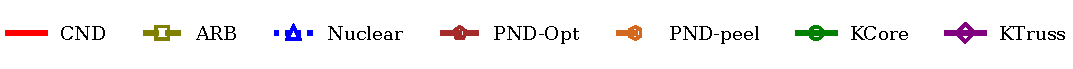
\includegraphics[width=0.9\linewidth]{figure/legend_algorithms_fixed_lines.pdf}

    \begin{minipage}[c]{0.02\textwidth}
    \centering
    \raisebox{2em}{\rotatebox{90}{\tiny \textbf{Time(s)}}} 
  \end{minipage}  \begin{subfigure}[t]{0.158\textwidth}
    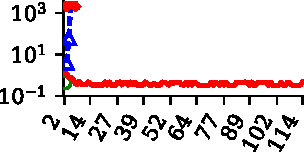
\includegraphics[width=\linewidth]{figure/com-dblp_r1_time_by_s_No_Hi.pdf}
    \caption{\myaddRA{DBLP$s\{r{=}1\}$}}
  \end{subfigure}\hfill
  \begin{subfigure}[t]{0.158\textwidth}
    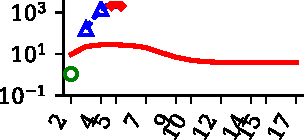
\includegraphics[width=\linewidth]{figure/com-youtube_r1_time_by_s_No_Hi.pdf}
    \caption{YT $s\{r{=}1\}$}
  \end{subfigure}\hfill
  \begin{subfigure}[t]{0.158\textwidth}
    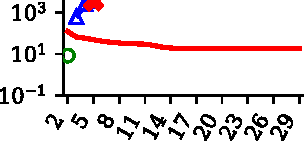
\includegraphics[width=\linewidth]{figure/soc-pokec-relationships_r1_time_by_s_No_Hi.pdf}
    \caption{PO $s\{r{=}1\}$}
  \end{subfigure}\hfill
  \begin{subfigure}[t]{0.158\textwidth}
    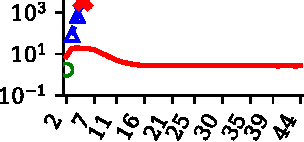
\includegraphics[width=\linewidth]{figure/web-Google_r1_time_by_s_No_Hi.pdf}
    \caption{GO $s\{r{=}1\}$}
  \end{subfigure}\hfill
  \begin{subfigure}[t]{0.158\textwidth}
    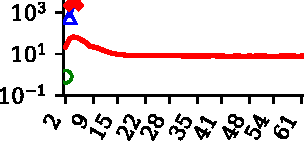
\includegraphics[width=\linewidth]{figure/web-Stanford_r1_time_by_s_No_Hi.pdf}
    \caption{STF $s\{r{=}1\}$}
  \end{subfigure}\hfill
  \begin{subfigure}[t]{0.158\textwidth}
    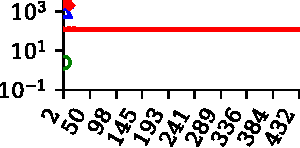
\includegraphics[width=\linewidth]{figure/web-it-2004_r1_time_by_s_No_Hi.pdf}
    \caption{WI $s\{r{=}1\}$}
  \end{subfigure}
  
  

    \begin{minipage}[c]{0.02\textwidth}
    \centering
    \raisebox{2em}{\rotatebox{90}{\tiny \textbf{Time(s)}}} 
  \end{minipage}  \begin{subfigure}[t]{0.158\textwidth}
    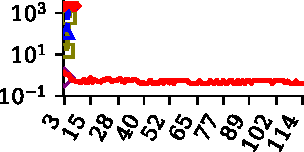
\includegraphics[width=\linewidth]{figure/com-dblp_r2_time_by_s_No_Hi.pdf}
    \caption{\myaddRA{DBLP$s\{r{=}2\}$}}
  \end{subfigure}\hfill
  \begin{subfigure}[t]{0.158\textwidth}
    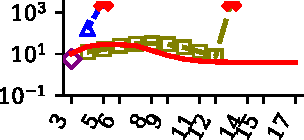
\includegraphics[width=\linewidth]{figure/com-youtube_r2_time_by_s_No_Hi.pdf}
    \caption{YT $s\{r{=}2\}$}
    \label{fig:youtube_r2_time_by_s}
  \end{subfigure}\hfill
  \begin{subfigure}[t]{0.158\textwidth}
    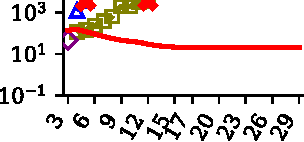
\includegraphics[width=\linewidth]{figure/soc-pokec-relationships_r2_time_by_s_No_Hi.pdf}
    \caption{PO $s\{r{=}2\}$}
  \end{subfigure}\hfill
  \begin{subfigure}[t]{0.158\textwidth}
    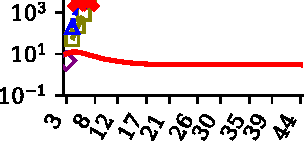
\includegraphics[width=\linewidth]{figure/web-Google_r2_time_by_s_No_Hi.pdf}
    \caption{GO $s\{r{=}2\}$}
  \end{subfigure}\hfill
  \begin{subfigure}[t]{0.158\textwidth}
    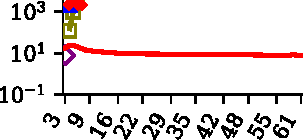
\includegraphics[width=\linewidth]{figure/web-Stanford_r2_time_by_s_No_Hi.pdf}
    \caption{STF $s\{r{=}2\}$}
  \end{subfigure}\hfill
  \begin{subfigure}[t]{0.158\textwidth}
    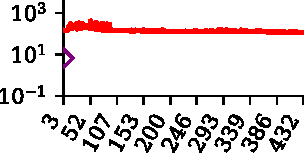
\includegraphics[width=\linewidth]{figure/web-it-2004_r2_time_by_s_No_Hi.pdf}
    \caption{WI $s\{r{=}2\}$}
  \end{subfigure}

  
  \caption{Running time (seconds) across $s$ without hierarchy for $r = 1$(a-f) and $r=2$(g-l).}
  \label{fig:r1r2_time_by_s}

  
    \begin{minipage}[c]{0.02\textwidth}
    \centering
    \raisebox{2em}{\rotatebox{90}{\tiny \textbf{Time(s)}}} 
  \end{minipage}  \begin{subfigure}[t]{0.158\textwidth}
    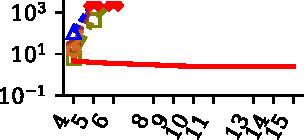
\includegraphics[width=\linewidth]{figure/com-dblp_r3_time_by_s_No_Hi.pdf}
    \caption{\myaddRA{DBLP$s\{r{=}3\}$}}
  \end{subfigure}\hfill
  \begin{subfigure}[t]{0.158\textwidth}
    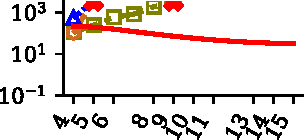
\includegraphics[width=\linewidth]{figure/soc-pokec-relationships_r3_time_by_s_No_Hi.pdf}
    \caption{PO $s\{r{=}3\}$}
  \end{subfigure}\hfill
  \begin{subfigure}[t]{0.158\textwidth}
    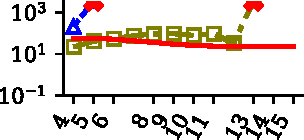
\includegraphics[width=\linewidth]{figure/com-youtube_r3_time_by_s_No_Hi.pdf}
    \caption{YT $s\{r{=}3\}$}
  \end{subfigure}\hfill
  \begin{subfigure}[t]{0.158\textwidth}
    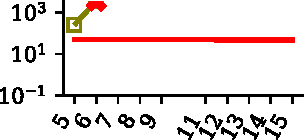
\includegraphics[width=\linewidth]{figure/com-dblp_r4_time_by_s_No_Hi.pdf}
    \caption{DBLP $s\{r{=}4\}$}
  \end{subfigure}\hfill
  \begin{subfigure}[t]{0.158\textwidth}
    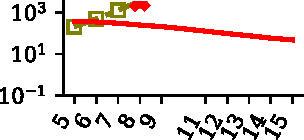
\includegraphics[width=\linewidth]{figure/soc-pokec-relationships_r4_time_by_s_No_Hi.pdf}
    \caption{PO $s\{r{=}4\}$}
  \end{subfigure}\hfill
  \begin{subfigure}[t]{0.158\textwidth}
    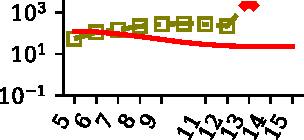
\includegraphics[width=\linewidth]{figure/com-youtube_r4_time_by_s_No_Hi.pdf}
    \caption{YT $s\{r{=}4\}$}
  \end{subfigure}

  

    \begin{minipage}[c]{0.02\textwidth}
    \centering
    \raisebox{2em}{\rotatebox{90}{\tiny \textbf{Time(s)}}} 
  \end{minipage}  \begin{subfigure}[t]{0.158\textwidth}
    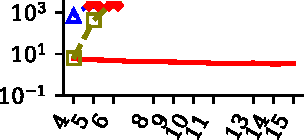
\includegraphics[width=\linewidth]{figure/com-dblp_r3_time_by_s.pdf}
    \caption{DBLP $s\{r{=}3\}$}
  \end{subfigure}\hfill
  \begin{subfigure}[t]{0.158\textwidth}
    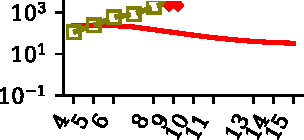
\includegraphics[width=\linewidth]{figure/soc-pokec-relationships_r3_time_by_s.pdf}
    \caption{PO $s\{r{=}3\}$}
  \end{subfigure}\hfill
  \begin{subfigure}[t]{0.158\textwidth}
    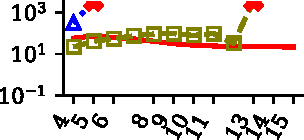
\includegraphics[width=\linewidth]{figure/com-youtube_r3_time_by_s.pdf}
    \caption{YT $s\{r{=}3\}$}
  \end{subfigure}\hfill
  \begin{subfigure}[t]{0.158\textwidth}
    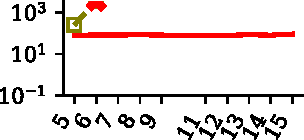
\includegraphics[width=\linewidth]{figure/com-dblp_r4_time_by_s.pdf}
    \caption{DBLP $s\{r{=}4\}$}
  \end{subfigure}\hfill
  \begin{subfigure}[t]{0.158\textwidth}
    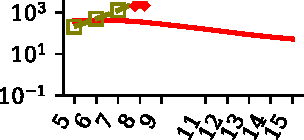
\includegraphics[width=\linewidth]{figure/soc-pokec-relationships_r4_time_by_s.pdf}
    \caption{PO $s\{r{=}4\}$}
  \end{subfigure}\hfill
  \begin{subfigure}[t]{0.158\textwidth}
    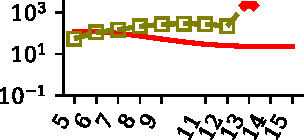
\includegraphics[width=\linewidth]{figure/com-youtube_r4_time_by_s.pdf}
    \caption{YT $s\{r{=}4\}$}
  \end{subfigure}

  
  \caption{Running time (seconds) across $s$ for $r \in \{3,4\}$(a-f without hierarchy; g-l with hierarchy).}
  \label{fig:time_by_s_r3_r4_combined}

  
    \begin{minipage}[c]{0.02\textwidth}
    \centering
    \raisebox{2em}{\rotatebox{90}{\tiny \textbf{Time(s)}}} 
  \end{minipage}  \begin{subfigure}[t]{0.158\textwidth}
      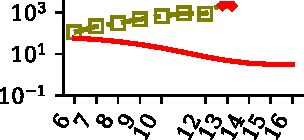
\includegraphics[width=\linewidth]{figure/com-youtube_r5_time_by_s_No_Hi.pdf}
      \caption{YT $s\{r{=}5\}$}
  \end{subfigure}\hfill
  \begin{subfigure}[t]{0.158\textwidth}
      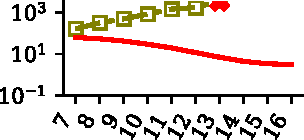
\includegraphics[width=\linewidth]{figure/com-youtube_r6_time_by_s_No_Hi.pdf}
      \caption{YT $s\{r{=}6\}$}
  \end{subfigure}\hfill
  \begin{subfigure}[t]{0.158\textwidth}
      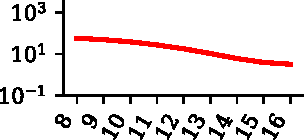
\includegraphics[width=\linewidth]{figure/com-youtube_r7_time_by_s_No_Hi.pdf}
      \caption{YT $s\{r{=}7\}$}
  \end{subfigure}\hfill
  \begin{subfigure}[t]{0.158\textwidth}
      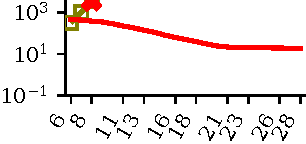
\includegraphics[width=\linewidth]{figure/soc-pokec-relationships_r5_time_by_s_no_hi-eps-converted-to.pdf}
      \caption{PO $s\{r{=}5\}$}
  \end{subfigure}\hfill
  \begin{subfigure}[t]{0.158\textwidth}
      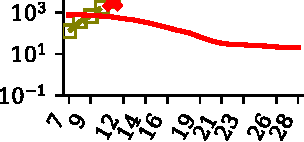
\includegraphics[width=\linewidth]{figure/soc-pokec-relationships_r6_time_by_s_no_hi.pdf}
      \caption{PO $s\{r{=}6\}$}
  \end{subfigure}\hfill
  \begin{subfigure}[t]{0.158\textwidth}
      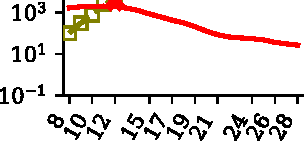
\includegraphics[width=\linewidth]{figure/soc-pokec-relationships_r7_time_by_s_no_hi.pdf}
      \caption{PO $s\{r{=}7\}$}
  \end{subfigure}

  
  \caption{Running time (seconds) across $s$ without hierarchy for $r \in \{5,6,7\}$.}
  \label{fig:time_by_s_r5_r7_combined}

    \begin{minipage}[c]{0.02\textwidth}
    \centering
    \raisebox{3em}{\rotatebox{90}{\tiny \textbf{Mem(MB)}}} 
  \end{minipage}  \begin{subfigure}[t]{0.158\textwidth}
    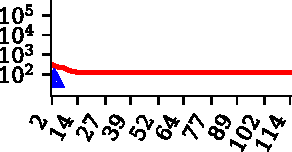
\includegraphics[width=\linewidth]{figure/com-dblp_r1_memory_by_s_no_hi.pdf}
    \caption{DBLP $s\{r{=}1\}$}
  \end{subfigure}\hfill
  \begin{subfigure}[t]{0.158\textwidth}
    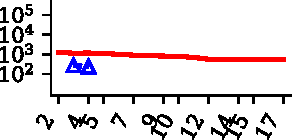
\includegraphics[width=\linewidth]{figure/com-youtube_r1_memory_by_s_no_hi.pdf}
    \caption{YT $s\{r{=}1\}$}
  \end{subfigure}\hfill
  \begin{subfigure}[t]{0.158\textwidth}
    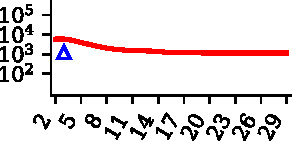
\includegraphics[width=\linewidth]{figure/soc-pokec-relationships_r1_memory_by_s_no_hi.pdf}
    \caption{PO $s\{r{=}1\}$}
  \end{subfigure}\hfill
  \begin{subfigure}[t]{0.158\textwidth}
    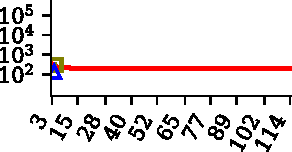
\includegraphics[width=\linewidth]{figure/com-dblp_r2_memory_by_s_no_hi.pdf}
    \caption{DBLP $s\{r{=}2\}$}
  \end{subfigure}\hfill
  \begin{subfigure}[t]{0.158\textwidth}
    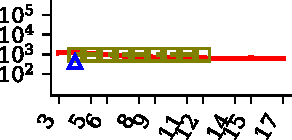
\includegraphics[width=\linewidth]{figure/com-youtube_r2_memory_by_s_no_hi.pdf}
    \caption{YT $s\{r{=}2\}$}
  \end{subfigure}\hfill
  \begin{subfigure}[t]{0.158\textwidth}
    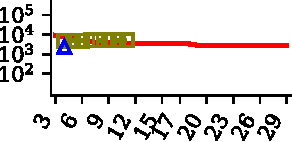
\includegraphics[width=\linewidth]{figure/soc-pokec-relationships_r2_memory_by_s_no_hi.pdf}
    \caption{PO $s\{r{=}2\}$}
  \end{subfigure}

    \begin{minipage}[c]{0.02\textwidth}
    \centering
    \raisebox{3em}{\rotatebox{90}{\tiny \textbf{Mem(MB)}}}
  \end{minipage}  
  \begin{subfigure}[t]{0.158\textwidth}
    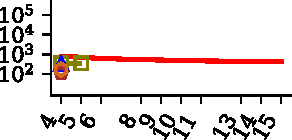
\includegraphics[width=\linewidth]{figure/com-dblp_r3_memory_by_s_no_hi.pdf}
    \caption{DBLP $s\{r{=}3\}$}
  \end{subfigure}\hfill
  \begin{subfigure}[t]{0.158\textwidth}
    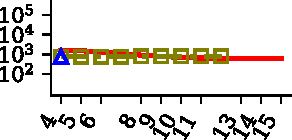
\includegraphics[width=\linewidth]{figure/com-youtube_r3_memory_by_s_no_hi.pdf}
    \caption{YT $s\{r{=}3\}$}
  \end{subfigure}\hfill
  \begin{subfigure}[t]{0.158\textwidth}
    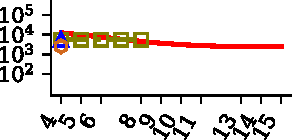
\includegraphics[width=\linewidth]{figure/soc-pokec-relationships_r3_memory_by_s_no_hi.pdf}
    \caption{PO $s\{r{=}3\}$}
  \end{subfigure}\hfill
  \begin{subfigure}[t]{0.158\textwidth}
    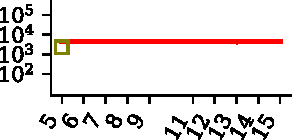
\includegraphics[width=\linewidth]{figure/com-dblp_r4_memory_by_s_no_hi.pdf}
    \caption{DBLP $s\{r{=}4\}$}
  \end{subfigure}\hfill
  \begin{subfigure}[t]{0.158\textwidth}
    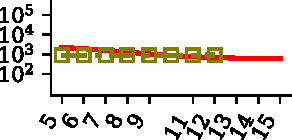
\includegraphics[width=\linewidth]{figure/com-youtube_r4_memory_by_s_no_hi.pdf}
    \caption{YT $s\{r{=}4\}$}
  \end{subfigure}\hfill
  \begin{subfigure}[t]{0.158\textwidth}
    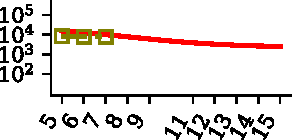
\includegraphics[width=\linewidth]{figure/soc-pokec-relationships_r4_memory_by_s_no_hi.pdf}
    \caption{PO $s\{r{=}4\}$}
  \end{subfigure}
  \caption{Time and Memory usage comparison for ($r \in \{1,2,3,4\}$).}
  \label{fig:mem_panel_b}
\end{figure*}
}


\section{Experimental Evaluation} \label{sec:exp}

\stitle{Hardware.} All algorithms are implemented in C++ and compiled using the g++ compiler with -O3 optimization. 
Experiments were conducted on a machine equipped with dual Intel(R) Xeon(R) Gold 6342 2.80GHz CPUs, 500GB of RAM, and running Ubuntu 22.

\input{sections/datasetTable}

% \renewcommand{\tabcolsep}{6pt}
\stitle{Datasets.} We evaluate our approach on six real-world datasets from diverse domains, including Co-authorship Networks: \textit{com-dblp} (cblp)~\cite{dblp}; Social Networks: \textit{soc-pokec} (pokec)~\cite{soc-pokec}, \textit{com-youtube} (youtube)~\cite{dblp}; and Web Graphs: \textit{web-Google} (google)~\cite{Stanford}, \textit{web-it-2004} (web-it)~\cite{nr}, \textit{web-Stanford} (stanford)~\cite{Stanford}. These datasets vary in size and structural characteristics, providing a comprehensive evaluation of our approach. Table~\ref{tab:graph-stats} summarizes the key statistics of these datasets.
% , including the number of vertices ($n$), number of edges ($m$), average degree, maximum degree, and the number of triangles. The datasets range from hundreds of thousands to over a million vertices, with varying edge densities and triangle counts, reflecting their diverse nature.

\stitle{Algorithms.} 
\myaddRA{
We compare our method with two state-of-the-art methods from the ARB line: the peeling framework \arb without hierarchy \cite{sotaPrveHierarchy}\footnote{\url{https://github.com/jeshi96/arb-nucleus-decomp}} and its hierarchy construction extension \cite{sotaHierarchy}\footnote{\url{https://github.com/jeshi96/arb-nucleus-hierarchy}}.
}
and the local $h$-index framework \nucleus from~\cite{LocalNuclear}\footnote{\url{https://github.com/sariyuce/nucleus}}.
\myaddRA{For \nucleus, in addition to its base implementation, we also evaluate its two optimized parallel variants available in the same repository: the peeling-based \nucleusP and the optimized local $h$-index \nucleusOPT.}
\arb, \nucleus and our method support hierarchy construction and core decomposition, while the \nucleusOPT and \nucleusP focus on decomposition.
% 
Notably, \arb does not support $r=1$ due to its algorithmic design. 
% 
Regarding \nucleus, its base implementation only supports the cases of $(r,s)=(1,3)$, $(1,4)$, $(2,3)$, and $(3,4)$.
% 这里紧接着说明优化版限制更死：只支持 (3,4)
\myaddRA{
Furthermore, \nucleusP and \nucleusOPT, are even more specialized and only support the case of $(r,s)=(3,4)$.
}
% 
Our method is publicly available.\footnote{\url{https://github.com/JamesZwq/nuclearSigmod/}}
%
Although these baselines differ in implementation details, they all follow the same exact peeling skeleton reviewed in Section~\ref{sec:existing_approaches} and rely on more reconstructive support-maintenance primitives.
%
They differ in implementation.
%
But they use the same exact peeling skeleton reviewed in Section~\ref{sec:existing_approaches}.
%
They also use more reconstructive support-maintenance primitives.
%
Our end-to-end comparison therefore evaluates both layers of our method.
%
It evaluates the counting/index layer provided by \cpi.
%
It also evaluates the DPCM update layer introduced in Section~\ref{sec:dpcm}.


\stitle{Metrics.}
Each experiment is executed three times, and we report the \emph{average} wall-clock runtime. 
A timeout of \textbf{3600\,seconds} (1 hour) is imposed; runs exceeding this limit are marked as \emph{out of time (OOT)} (denoted by $\textcolor{red}{\boldsymbol{\times}}$ in figures) and excluded from the averages.

\stitle{Evaluation Questions.}
Our experiments are designed to answer four questions.
%
\textbf{Q1:} Does the combined \cpi\,+\,DPCM framework consistently outperform prior exact peeling methods across different values of $r$ and $s$?
%
\textbf{Q2:} Do the three DPCM instantiations yield the expected regime-specific benefits, namely counter-state updates for $r{=}1$, edge-contribution updates for $r{=}2$, and conflict-state pruning for $r{\ge}3$?
%
\textbf{Q3:} How much of the gain comes from avoiding reconstructive support maintenance, as opposed to merely changing the underlying representation?
%
\textbf{Q4:} Does the same framework also preserve the efficiency advantage when hierarchy construction is included?
%
Questions~Q1--Q3 separate the two layers of our approach.
%
Q1 studies the end-to-end effect of combining representation and maintenance.
%
Q2 studies whether the regime-specific sufficient states predicted by DPCM appear in practice.
%
Q3 separates the compression benefit of \cpi from the update benefit of differential maintenance.
%
Q4 checks whether the same advantages remain after we add connectivity maintenance for hierarchy construction.

% In line plots, \emph{out-of-time (OOT)} cases are indicated by a red patterned band at the timeout threshold; accordingly, any red pattern along the top of the plot denotes an OOT case. And for all following experiments, we run the experiment until the first timeout for all methods(e.g., if one method times out at $s=4$, we will not run the experiment for $s>4$ for this method).


% \expsection{Running Time $(r \leq 2)$}
% % 在本试验中, 我们运行了table~\ref{tab:graph-stats}中列出的六个真实数据集, 并分别测试了在没有hierarchical构建的$r=1$和$r=2$的情况. 对于每个数据集, 我们将参数$s$从较小的值(例如$r=1$时的$s=3$, $r=2$时的$s=4$)逐步增加到数据集中观察到的最大团大小. 实验结果如图~\ref{fig:dblp_r1_time_by_s}所示. 我们的算法CND在任何数据集中, 随着$s$的增加, 运行时间并无显著增长, 并且曲线趋于平稳, 我们高效的计算了所有s的结果. 
% In this experiment, we evaluate both $r=1$ and $r=2$ cases without hierarchical construction across six datasets. 
% For each dataset, we vary the parameter $s$ from small values (e.g., $s=3$ for $r=1$ and $s=4$ for $r=2$) up to the maximum clique size in the dataset. 
% The experimental results are shown in Figure~\ref{fig:r1r2_time_by_s}. 
% Across all datasets, as $s$ increases, the runtime of our \cbnd algorithm exhibits minimal growth and quickly stabilizes, demonstrating its ability to efficiently compute results for all values of $s$.
% % 算法\arb和算法\nucleus在大多数情况下, 运行时间都随着s的增加有着显著增长并且快速timeout. 算法\arb在youtube 数据集r=2的时候有着不寻常的表现, 因为youtube 数据集的最大团大小为17, 很小, 所以我们的算法在这个数据集上的优势并不太明显, 但是其在r=2,s=13时也timeout, 对比之下, CND只是用了30秒就完成了计算.
% \arb and \nucleus exhibit substantial runtime growth as $s$ increases in most cases, often leading to rapid timeouts. 
% Notably, \arb performs better on the \textsc{YouTube} dataset for $r=2$, as its maximum clique size is small (i.e., $17$). 
% Consequently, the performance gap between \arb and our algorithm is narrower on this dataset. 
% However, \arb still times out at $r=2, s=13$, whereas \cbnd completes the computation in only 30 seconds.
% % 
% % 在数据集web-it-2004上, ARB在r=2的任何s下都timeout了, 而CND在r=2,s=4的情况下只用了240秒就完成了计算, 并且顺利的计算了所有s的结果.
% On the \textsc{web-it-2004} dataset, \arb times out for all values of $s$ when $r=2$, whereas \cbnd completes the computation in only 240 seconds for $r=2, s=4$, successfully producing results for all values of $s$.
% % 在本试验中 CND比ARB和NUCLEUS分别有平均30x和20x的加速, 对快达到了342x在dblp数据集的r=2,s=5的情况下.
% \cbnd achieves average speedups of 30x and 20x over \arb and \nucleus, respectively, with a maximum speedup of 342x observed on the DBLPdataset for $r=2, s=5$.

\expsection{Running Time $(r \leq 2)$}
We evaluate $r\in\{1,2\}$ without hierarchy on six datasets, sweeping $s$ from $3/4$ up to each dataset's maximum clique size (Figure~\ref{fig:r1r2_time_by_s}).
%
These results answer Q1.
%
They also answer the low-order part of Q2.
%
\cbnd shows little sensitivity to $s$: curves are essentially flat across datasets.
%
This is the behavior predicted by counter-state and edge-contribution DPCM.
%
Once \cpi compactly represents the clique space, support updates do not need to reconstruct large affected local neighborhoods as $s$ grows.
%
In contrast, \arb and \nucleus grow rapidly with $s$ and often time out.
%
Atypical is \texttt{com-youtube} at $r{=}2$ (max clique $17$), where the gap narrows; even there, \arb times out at $s{=}13$ while \cbnd finishes in about 30s.
%
On \texttt{web-it-2004} ($r{=}2$), \arb times out for all $s$, whereas \cbnd completes from $s{=}4$ onward (e.g., 240s at $s{=}4$) and handles the full range.
%
On comparable settings, \cbnd is about $6.3\times$ faster than \arb and about $18.0\times$ faster than \nucleus.
%
The largest gap is above two orders of magnitude.
% 
% 我们也与目前最先进的kcore和ktruss的算法进行了对比, 
\myaddRA{
We further compare against specialized single-thread baselines for the two canonical special cases: $k$-core ($(r,s)=(1,2)$)\cite{batagelj2003omalgorithmcoresdecomposition} and $k$-truss ($(r,s)=(2,3)$)\cite{wang2012truss}. 
On \texttt{com-dblp}, \cbnd runs in $1.21$s for $(1,2)$ vs.\ $0.45$s for $k$-core, and $1.31$s for $(2,3)$ vs.\ $0.78$s for $k$-truss. 
This result shows that our combined CPI+DPCM framework has only modest overhead on the special cases.
%
It still keeps the advantage of avoiding explicit clique enumeration.
%
It also remains effective as $s$ increases.
}


\expsection{Running Time $(r \in \{3,4\})$}
We evaluate $r\in\{3,4\}$ on three datasets, with and without hierarchy (Figure~\ref{fig:time_by_s_r3_r4_combined}).

\expsubsection{Without Hierarchy}
Figure~\ref{fig:time_by_s_r3_r4_combined} compares \cbnd with \nucleus and \arb. 
%
This part mainly answers the general-regime side of Q2.
%
It also helps answer Q3.
%
As with $r\le 2$, \cbnd is nearly insensitive to $s$, curves stay essentially flat, while \arb (and \nucleus) grow rapidly with $s$ and frequently time out. 
%
The key difference is that the gain here does not come from simple counter or edge states.
%
It comes from conflict-state DPCM.
%
Dead paths are pruned early.
%
Only the surviving residual paths need further exact maintenance.
%
On comparable settings, \cbnd is about $2.8\times$ faster than \arb and about $4.6\times$ faster than the base \nucleus implementation.
%
The largest speedup reaches $106.7\times$ on \texttt{com-dblp} at $r{=}3, s{=}5$.
% 新增对比
\myaddRA{
We also evaluate the specialized algorithms \nucleusP and \nucleusOPT for $(r,s)=(3,4)$. 
On \texttt{com-dblp}, \cbnd achieves $3.2\times$ and $5.5\times$ speedups, respectively.
% 简短的原因分析
However, \cbnd is less effective on graphs with small max cliques but large average degrees (e.g., \texttt{soc-pokec} and \texttt{web-Google}).
% 在这两个数据集中, (r,s)=(3,4)的时候,\nucleusOPT, \nucleusP和\arb均比CND快了1点多倍, 当然随着s的增加, 例如(3,5)和(4,5)的时候,CND有迅速获得了强大的优势.
In these datasets, for $(r,s)=(3,4)$, \nucleusOPT, \nucleusP, and \arb are all around $1\times$ faster than \cbnd; however, as $s$ increases (e.g., $(3,5)$ and $(4,5)$), \cbnd quickly gains a strong advantage.
% 这是因为在
In such cases, the enumeration cost for baselines is naturally low, while the dense connectivity increases the maintenance overhead of our index.
}

\expsubsection{With Hierarchy}
Figure~\ref{fig:time_by_s_r3_r4_combined}.2 shows the hierarchical setting.
%
This addresses Q4.
%
The same trend appears in the hierarchical setting.
%
\cbnd stays stable as $s$ increases, whereas the baselines often slow down or time out.
%
On comparable settings, \cbnd is about $2.6\times$ faster than \arb and about $18.4\times$ faster than \nucleus.
%
The largest speedup reaches $146.6\times$ on \texttt{com-dblp} at $r{=}3, s{=}4$.

\expsection{Running Time $(r \in \{5,6,7\})$}
\myaddRA{
Figure~\ref{fig:time_by_s_r5_r7_combined} reports the efficiency for higher-order nucleus decomposition on \texttt{soc-pokec} and \texttt{com-youtube}. 
As $r$ increases, \cbnd maintains a robust and relatively flat performance curve. 
In contrast, \arb exhibits a non-monotonic trend. 
On \texttt{soc-pokec}, the speedup of \cbnd over \arb narrows at medium $r$ (e.g., dropping to $1.0\times$ at $r{=}6$), as stricter constraints shrink the search space for enumeration.
However, this resilience is transient. 
At $r{=}7$, \arb degrades sharply on \texttt{soc-pokec} (e.g., taking 2590s at $s{=}11$ vs. 31s for \cbnd, an $83\times$ difference) and eventually times out. 
The situation is even worse on \texttt{com-youtube}, where \arb fails to complete entirely at $r{\ge}7$.
This demonstrates that while enumeration-based frameworks can transiently benefit from filtered search spaces, they remain fundamentally fragile to high-order complexity.
}


\begin{figure}
  \centering
  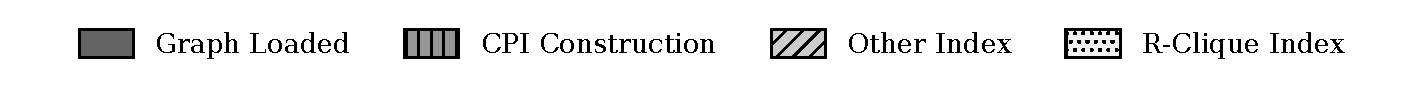
\includegraphics[width=0.7\textwidth]{figure/breakdown_memory_legend.pdf}
  

  \begin{subfigure}[t]{0.32\textwidth}
      \centering
      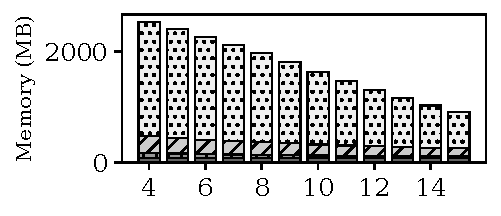
\includegraphics[width=\linewidth]{figure/breakdown_memory_Google.pdf}
      \caption{GO $s\{r{=}3\}$}
      \label{fig:bd_google_mem}
  \end{subfigure}\hfill
  \begin{subfigure}[t]{0.32\textwidth}
      \centering
      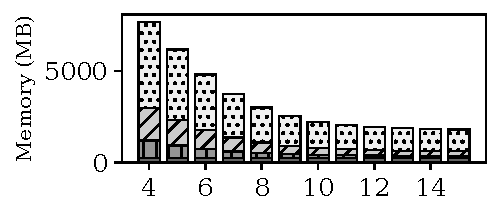
\includegraphics[width=\linewidth]{figure/breakdown_memory_Pokec.pdf}
      \caption{PO $s\{r{=}3\}$}
      \label{fig:bd_pokec_mem}
  \end{subfigure}\hfill
  \begin{subfigure}[t]{0.32\textwidth}
      \centering
      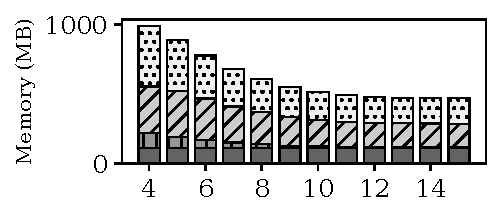
\includegraphics[width=\linewidth]{figure/breakdown_memory_Youtube.pdf}
      \caption{YT $s\{r{=}3\}$}
      \label{fig:bd_youtube_mem}
  \end{subfigure}
    \caption{Breakdown of \textbf{memory usage} on different datasets ($r=3$) as $s$ varies. }
  \label{fig:breakdown_mem}
  
  \centering
  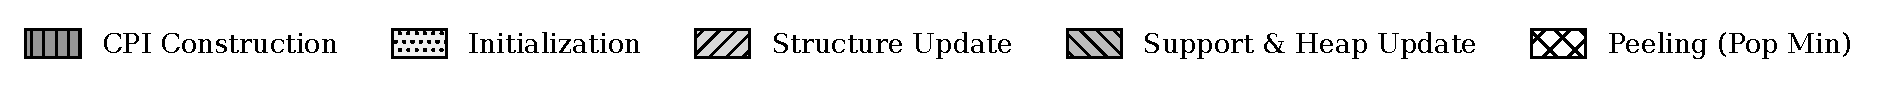
\includegraphics[width=0.9\textwidth]{figure/breakdown_legend.pdf}

  \begin{subfigure}[t]{0.32\textwidth}
      \centering
      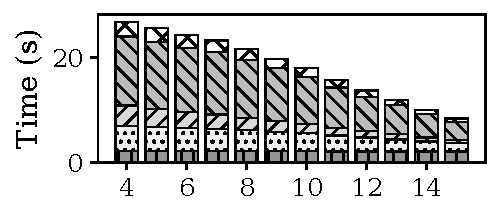
\includegraphics[width=\linewidth]{figure/breakdown_Google.pdf}
      \caption{GO $s\{r{=}3\}$}
      \label{fig:bd_google_time}
  \end{subfigure}\hfill
  \begin{subfigure}[t]{0.32\textwidth}
      \centering
      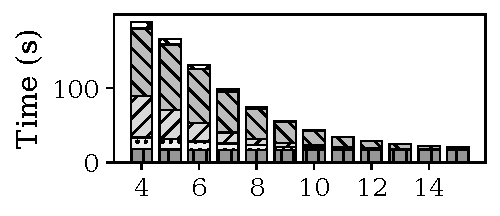
\includegraphics[width=\linewidth]{figure/breakdown_Pokec.pdf}
      \caption{PO $s\{r{=}3\}$}
      \label{fig:bd_pokec_time}
  \end{subfigure}\hfill
  \begin{subfigure}[t]{0.32\textwidth}
      \centering
      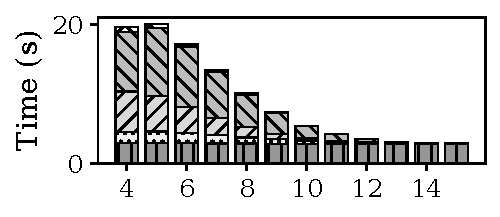
\includegraphics[width=\linewidth]{figure/breakdown_Youtube.pdf}
      \caption{YT $s\{r{=}3\}$}
      \label{fig:bd_youtube_time}
  \end{subfigure}
    \caption{Breakdown of \textbf{running time} on different datasets ($r=3$) as $s$ varies. }
  \label{fig:breakdown_time}
\end{figure}


\expsection{Memory Usage}
\myaddRA{
Figures~\ref{fig:mem_panel_b}(a-i) and~\ref{fig:breakdown_mem} analyze memory consumption. Our method and the state-of-the-art \arb have comparable memory usage overall. As $s$ increases, our memory decreases while \arb stays nearly constant.
This is because larger $s$ leaves fewer valid $r$-cliques: many $r$-cliques contain no $s$-cliques. We do not store such $r$-cliques, whereas \arb cannot reliably pre-filter them and thus maintains states for all $r$-cliques.
% 
For $r{=}1$, our method uses more memory than \nucleus but is substantially faster. 
On \texttt{com-dblp} ($r{=}1,s{=}4$), \nucleus uses 73MB and takes 62.8s, while our method uses 253MB ($\approx3.5\times$) and finishes in 0.8s (77.7$\times$ speedup). 
On \texttt{web-Stanford} ($r{=}1,s{=}3$), \nucleus uses 126MB and runs for 596s, while our method uses 656MB and completes in 55s (x10.8$\times$ speedups). 
Thus, even in low-order settings where baselines are optimized, the additional memory translates to significant performance gains.
}
\myaddRC{
Figure~\ref{fig:breakdown_mem} further breaks down \cbnd's memory usage across datasets and $(r,s)$ settings. Most memory is spent on storing $r$-cliques rather than CPI, indicating that \cpi itself is memory-efficient.
}




\expsection{Runtime Breakdown}
\myaddRA{
Figure~\ref{fig:breakdown_time} reports the runtime breakdown of \cbnd across datasets. 
We decompose the total time into five components:
\textit{CPI Construction},
\textit{Init} (initial $r$-clique enumeration and support counting),
\textit{Structure Update} (updating CPI structure during peeling),
\textit{Support} (updating $s$-clique supports via neighbor intersections),
and \textit{Peeling} (heap maintenance and PopMin operations).
Overall, \textit{Init} and \textit{Support} are the main cost drivers.
On \texttt{com-dblp} ($r{=}4$), \textit{Init} accounts for 36.2\%--38.0\% and \textit{Support} for 17.7\%--18.3\% (two runs); on \texttt{web-Google} ($r{=}4$), \textit{Support} becomes the bottleneck (39.9\%) while \textit{Init} is 14.5\% (and \textit{Peeling} is 27.3\%).
These results indicate that runtime is primarily governed by clique enumeration and neighbor intersections (Init/Support), while CPI construction/maintenance and heap-based peeling contribute the remaining overhead.
%
For Q3, the important observation is that \textit{Structure Update} remains a secondary cost across datasets.
%
This is consistent with DPCM: once the initial representation is built, most dynamic work is handled by localized differential updates rather than repeated reconstructive maintenance of the full affected clique space.
}


\begin{figure}

  
  \centering
  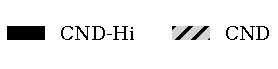
\includegraphics[width=0.2\linewidth]{figure/cbs_vs_nohi_comp_legend_long.pdf}
  

  \begin{subfigure}[t]{0.243\textwidth}
    \centering 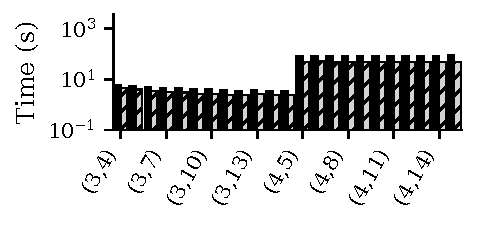
\includegraphics[width=\linewidth]{figure/abc_comp_com-dblp_time_by_rs_long.pdf}
    \caption{DBLP($r$,$s$)}
  \end{subfigure}
  \begin{subfigure}[t]{0.243\textwidth}
    \centering 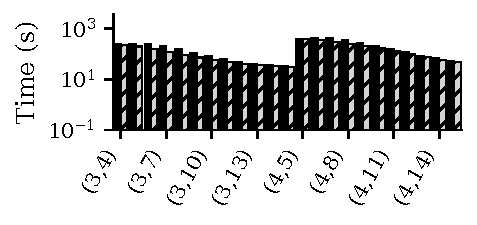
\includegraphics[width=\linewidth]{figure/abc_comp_soc-pokec-relationships_time_by_rs_long.pdf}
    \caption{PO ($r$,$s$)}
  \end{subfigure}
  \begin{subfigure}[t]{0.243\textwidth}
    \centering 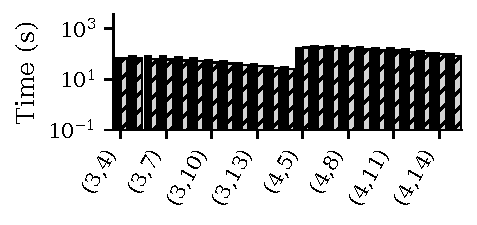
\includegraphics[width=\linewidth]{figure/abc_comp_web-Google_time_by_rs_long.pdf}
    \caption{GO ($r$,$s$)}
  \end{subfigure}
  \begin{subfigure}[t]{0.243\textwidth}
    \centering 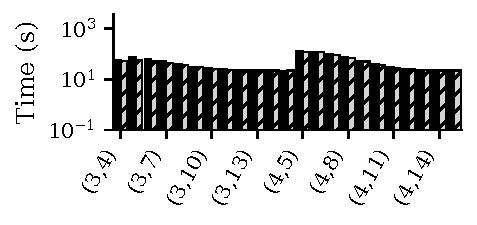
\includegraphics[width=\linewidth]{figure/abc_comp_com-youtube_time_by_rs_long.pdf}
    \caption{YT ($r$,$s$)}
  \end{subfigure}

  \caption{Time (in seconds) Hierarchical vs Non-Hierarchical with varying $r,s$.}
  \label{fig:hierarchy_vs_nohierarchy}
\end{figure}

\begin{figure}
  \centering
  
\includegraphics[width=0.50\linewidth]{figure/legend_leafCount_generic.pdf}
    
  \begingroup
  \setcounter{panel}{0}
  \begin{minipage}[c]{0.02\textwidth}
    \centering
      \raisebox{4em}{\rotatebox{90}{\tiny \textbf{Count}}} 
  \end{minipage}    \begin{subfigure}[t]{0.16\textwidth} 
      \centering 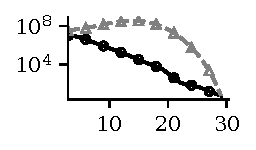
\includegraphics[width=\linewidth]{figure/leaf_clique_soc-pokec-relationships.pdf}
      % \caption{$k$-clique \\ (pokec)}
      \caption{PO $k$-clique}
    \end{subfigure}\hfill
    \begin{subfigure}[t]{0.16\textwidth}
      \centering 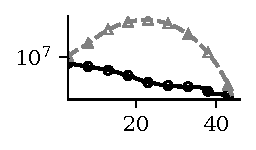
\includegraphics[width=\linewidth]{figure/leaf_clique_web-Google.pdf}
      % \caption{$k$-clique \\ (Google)}
      \caption{GO $k$-clique}
    \end{subfigure}\hfill
    \begin{subfigure}[t]{0.16\textwidth}
      \centering 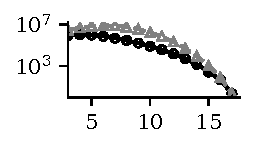
\includegraphics[width=\linewidth]{figure/leaf_clique_com-youtube.pdf}
      % \caption{$k$-clique \\ (youtube)}
      \caption{YT $k$-clique}
    \end{subfigure}\hfill
    \begin{subfigure}[t]{0.16\textwidth}
      \centering 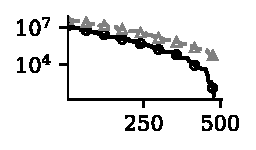
\includegraphics[width=\linewidth]{figure/leafCount_soc-pokec-relationships_34.pdf}
      % \caption{\#Iter \\ (pokec)}
      \caption{PO \#Iter}
    \end{subfigure}\hfill
    \begin{subfigure}[t]{0.16\textwidth}
      \centering 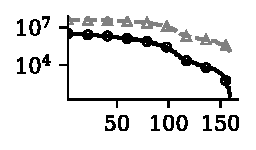
\includegraphics[width=\linewidth]{figure/leafCount_web-Google_34.pdf}
      % \caption{\#Iter \\ (Google)}
      % \caption{\#Iter \\ (GO)}
      \caption{GO \#Iter}
    \end{subfigure}\hfill
    \begin{subfigure}[t]{0.16\textwidth}
      \centering 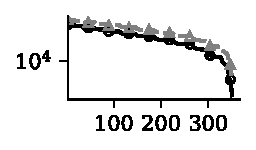
\includegraphics[width=\linewidth]{figure/leafCount_com-youtube_34.pdf}
      % \caption{\#Iter \\ (youtube)}
      \caption{YT \#Iter}
    \end{subfigure}\hfill

  
  \caption{CPI \#Paths vs.\ \#s-cliques for $r=3, s=4$.}
    \label{fig:leafcount}
    
  \endgroup
\end{figure}





\expsection{Ablation Study for $r \in {1,2}$}
\myaddRA{
Figure~\ref{fig:ablation_exp} reports an ablation study for $r\in\{1,2\}$.
To reduce the overhead of generic clique enumeration at low orders, we add specialized optimizations for $r{=}1$ and $r{=}2$.
Compared with the generic baseline (\texttt{CBS3}), the optimized version (\texttt{CBS-noHi}) is consistently faster:
on \texttt{com-dblp} with $r{=}2,s{=}4$, runtime drops from 1.57s to 1.04s (1.5$\times$), and for $r{=}1$ we observe $\approx$1.3$\times$ speedup.
Memory usage remains similar since the optimization only changes \cpi updates and does not change the stored \cpi structure.
%
This directly supports Q2: once the same \cpi representation is fixed, regime-specific DPCM operators still contribute additional gains.
}




\begin{figure}
  \centering
      
\includegraphics[width=0.8\linewidth,trim={0 8pt 0 26pt},clip]{figure/legend_sort_options.pdf}
  
      \setlength{\tabcolsep}{0pt} 
    \begin{subfigure}[t]{0.162\textwidth}
    \centering
    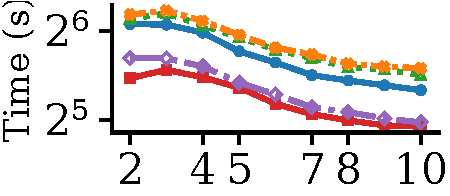
\includegraphics[width=\linewidth]{figure/r1_time.pdf}
    \caption{$s\{r{=}1\}$ \\ Time}
    \label{fig:ord_r1_time}
  \end{subfigure}\hfill
  \begin{subfigure}[t]{0.162\textwidth}
    \centering
    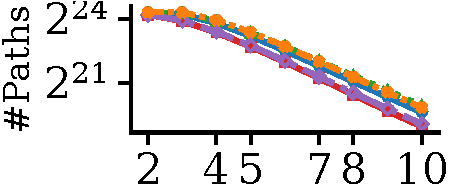
\includegraphics[width=\linewidth]{figure/r1_leafs.pdf}
    \caption{$s\{r{=}1\}$ \\ \#Paths}
    \label{fig:ord_r1_mem}
  \end{subfigure}\hfill
  \begin{subfigure}[t]{0.162\textwidth}
    \centering
    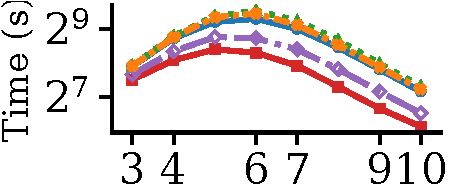
\includegraphics[width=\linewidth]{figure/r2_time.pdf}
    \caption{$s\{r{=}2\}$ \\ Time}
    \label{fig:ord_r2_time}
  \end{subfigure}\hfill
  \begin{subfigure}[t]{0.162\textwidth}
    \centering
    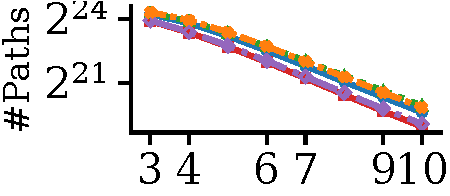
\includegraphics[width=\linewidth]{figure/r2_leafs.pdf}
    \caption{$s\{r{=}2\}$ \\ \#Paths}
    \label{fig:ord_r2_mem}
  \end{subfigure}\hfill
    \begin{subfigure}[t]{0.162\textwidth}
    \centering
    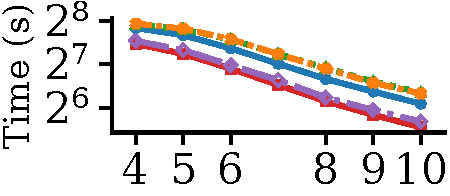
\includegraphics[width=\linewidth]{figure/r3_time.pdf}
    \caption{$s\{r{=}3\}$ \\ Time}
    \label{fig:ord_r3_time}
  \end{subfigure}\hfill
  \begin{subfigure}[t]{0.162\textwidth}
    \centering
    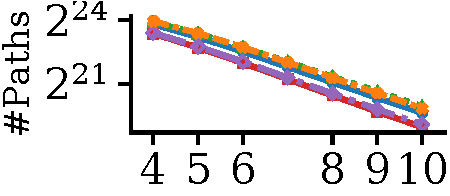
\includegraphics[width=\linewidth]{figure/r3_leafs.pdf}
    \caption{$s\{r{=}3\}$ \\ \#Paths}
    \label{fig:ord_r3_mem}
  \end{subfigure}\hfill

    \caption{Impact of different vertex ordering strategies in soc-pokec}
  \label{fig:order_exp}
  
\end{figure}


\expsection{Hierarchy vs.\ No Hierarchy}
% 在本试验中我们对比了我们的算法CND在有和没有hierarchical构建的情况下的性能差异.
% In this experiment, we compare the performance of our \cbnd algorithm with and without hierarchical construction.
% 图~\ref{fig:hierarchy_vs_nohierarchy}展示了在$r=3$和$r=4$的情况下, 我们的算法CND在有和没有hierarchical构建的情况下的对比. 我们选择了数据集dblp, soc-pokec-relationships和web-Google作为代表.
% Figure~\ref{fig:hierarchy_vs_nohierarchy} illustrates the comparison of our \cbnd algorithm with and without hierarchical construction for $r=3$ and $r=4$. We select the datasets \texttt{Youtube}, \texttt{soc-pokec}, and \texttt{web-Google} as representatives.
% Across all datasets, the runtimes of our \cbnd algorithm with and without hierarchical construction are very close. On average, the hierarchical version takes about 10\% more time than the non-hierarchical version. This indicates that our \cbnd algorithm exhibits very stable performance regardless of whether hierarchical construction is employed.
Figure~\ref{fig:hierarchy_vs_nohierarchy} compares \cbnd with and without hierarchical construction for $r\in\{3,4\}$ on \texttt{Youtube}, \texttt{soc-pokec}, and \texttt{web-Google}.
Across all three datasets, the two variants have nearly identical runtimes; the hierarchical version is about 10\% slower on average.
This indicates that our \cbnd algorithm exhibits very stable performance regardless of whether hierarchical construction is employed.
%
This confirms Q4: once \cpi and DPCM are in place, maintaining $s$-connectivity for hierarchy adds only modest overhead.




\begin{figure}
  \centering

    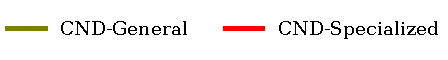
\includegraphics[width=0.4\linewidth]{figure/special_cbs_comparison_legend-eps-converted-to.pdf}
  
  \captionsetup[subfigure]{font=tiny, skip=0pt}
  
  \begin{subfigure}[t]{0.24\textwidth}
    \centering
    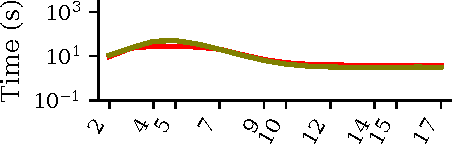
\includegraphics[width=\linewidth]{figure/special_com-youtube_r1_time.pdf}
    \caption{YT $s\{r{=}1\}$}
  \end{subfigure}\hfill
  \begin{subfigure}[t]{0.24\textwidth}
    \centering
    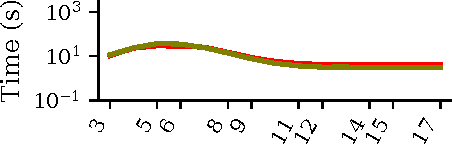
\includegraphics[width=\linewidth]{figure/special_com-youtube_r2_time.pdf}
    \caption{YT $s\{r{=}2\}$}
  \end{subfigure}\hfill
  \begin{subfigure}[t]{0.24\textwidth}
    \centering
    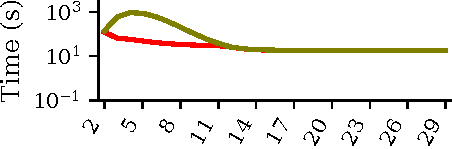
\includegraphics[width=\linewidth]{figure/special_soc-pokec-relationships_r1_time.pdf}
    \caption{PO $s\{r{=}1\}$}
  \end{subfigure}\hfill
  \begin{subfigure}[t]{0.24\textwidth}
    \centering
    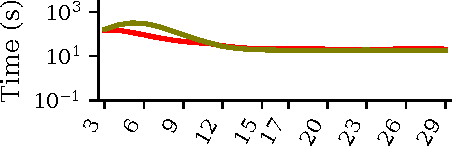
\includegraphics[width=\linewidth]{figure/special_soc-pokec-relationships_r2_time.pdf}
    \caption{PO $s\{r{=}2\}$}
  \end{subfigure}\hfill
  \begin{subfigure}[t]{0.24\textwidth}
    \centering
    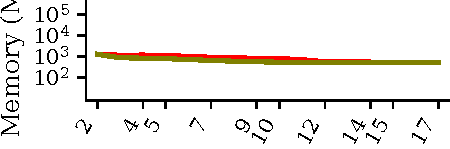
\includegraphics[width=\linewidth]{figure/special_com-youtube_r1_mem.pdf}
    \caption{YT $s\{r{=}1\}$}
  \end{subfigure}\hfill
  \begin{subfigure}[t]{0.24\textwidth}
    \centering
    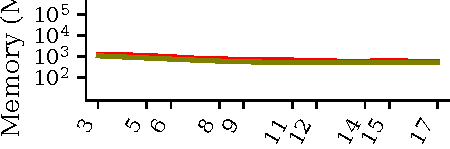
\includegraphics[width=\linewidth]{figure/special_com-youtube_r2_mem.pdf}
    \caption{YT $s\{r{=}2\}$}
  \end{subfigure}\hfill
  \begin{subfigure}[t]{0.24\textwidth}
    \centering
    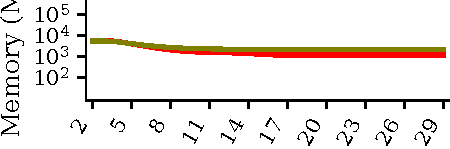
\includegraphics[width=\linewidth]{figure/special_soc-pokec-relationships_r1_mem.pdf}
    \caption{PO $s\{r{=}1\}$}
  \end{subfigure}\hfill
  \begin{subfigure}[t]{0.24\textwidth}
    \centering
    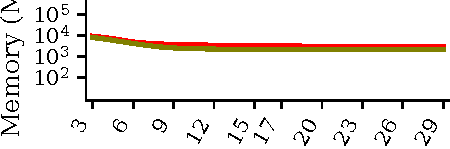
\includegraphics[width=\linewidth]{figure/special_soc-pokec-relationships_r2_mem.pdf}
    \caption{PO $s\{r{=}2\}$}
  \end{subfigure}\hfill
                                                                                  

    \caption{Comparison of execution time for \cbnd general vs. specialized algorithms.}
  \label{fig:ablation_exp}
  
\end{figure}

\expsection{Node Orderings}
\myaddRB{
We evaluate five vertex orderings on \texttt{soc-pokec} (Figure~\ref{fig:order_exp}): \texttt{origin}, \texttt{degree}/\texttt{degreeR}, and \texttt{degen}/\texttt{degenR}.
Across all tested $s$ (2--10 for $r{=}1$, 3--10 for $r{=}2$, and 4--10 for $r{=}3$), \texttt{degen} is consistently the best overall.
Averaged over all tested $s$, \texttt{degen} is
1.39$\times$ faster than \texttt{origin} for $r{=}1$ (52.6s $\rightarrow$ 37.9s),
1.86$\times$ for $r{=}2$ (392.5s $\rightarrow$ 210.5s), and
1.37$\times$ for $r{=}3$ (139.8s $\rightarrow$ 102.1s).
% The second-best choice is typically \texttt{degree}, but \texttt{degen} still yields an extra 7.3\% / 23.3\% / 6.0\% speedup for $r{=}1/2/3$.
In contrast, the reverse orderings are consistently the slowest: \texttt{degenR}/\texttt{degreeR} are 1.52--2.11$\times$ slower than \texttt{degen} on average.
% 
Moreover, \texttt{degen} shrinks the CPI: compared with \texttt{origin}, it reduces CPI \#paths by 28.3\% / 30.9\% / 32.5\% on average for $r{=}1/2/3$ (up to 37.2\% at $s{=}10$), translating to average memory savings of 0.82 / 0.67 / 0.37\,GB.
For example, at $r{=}1,s{=}3$, \texttt{degen} reduces CPI \#paths from 19.78M to 15.82M ($-20\%$), lowering memory from 6.35\,GB to 5.18\,GB ($-1.17$\,GB) and runtime from 67.2s to 47.3s.
We therefore adopt \texttt{degen} as the default ordering strategy.
}


\expsection{\#Paths vs. \#$s$-Cliques}
Across peeling iterations, we compare the number of CPI paths with the number of $s$-cliques (Figure~\ref{fig:leafcount}) for $(r,s)=(3,4)$ on three datasets. 
On all datasets and in almost all iterations, the path count is far below $|K_s|$, indicating that CPI stays compact and output-sensitive.
Moreover, the path count is flat or decreasing over time, suggesting that path splits are non-inflationary.
A mild exception is \texttt{com-youtube} at $s{=}4$, whose sparsity and small maximum clique size ($\omega{=}17$) narrow the gap, consistent with its more modest speedups (Figure~\ref{fig:youtube_r2_time_by_s}).
%
This experiment isolates the representation side of Q3: even before considering differential updates, \cpi already compresses the active clique space substantially.


% 
% \expsection{Scalability}
% We evaluate scalability on \texttt{web-Google} and \texttt{youtube}(Figure~\ref{fig:scalability_time_memory}).
% For each graph, we run $r\in\{1,2,3\}$ and sweep $s$ up to 15, reporting wall-clock time. 
% We vary workload by subsampling edges to 20--100\% of the input; the curves are labeled by sampling ratios. 
% Runtime curves are cleanly ordered (20\% $<$ 40\% $<$ 60\%$< $80\%$<$100\%), indicating near-linear dependence on graph size. 
% Moreover, time consistently decreases as $s$ increases, and this trend holds even at 100\% input, demonstrating robust full-scale performance. 
% Overall, \cbnd scales smoothly with both graph size and parameters.

\myaddRA{
\expsection{Stress Test}
% To evaluate limits under combinatorial explosion, To probe the limits under combinatorial explosion, we stress-test synthetic graphs ($N{=}1000$) generated via incremental clique injection, where clique sizes follow a truncated power-law and the injected clique size is capped at 100; we vary the edge density from $p{=}0.01$, yielding $deg_{\text{avg}}\approx p|V|$.
 To evaluate limits under combinatorial explosion, We stress-test on $N{=}1000$ synthetic graphs built by incremental clique injection: clique sizes are sampled from a truncated power-law (max size $100$), and density is increased from $p{=}0.01$, yielding $\bar d \approx p(|V|-1)$.
It is worth noting that our starting density $p{=}0.01$ is already orders of magnitude higher than typical real-world networks (e.g., \texttt{com-dblp} has $p{\approx}2{\times}10^{-5}$), creating a rigorous worst-case scenario.
Experimental results ($r{\in}\{4,5\}, s{\in}\{5..9\}$) show that \cbnd remains robust in these settings.
As complexity increases, the baseline \arb collapses rapidly: for $(r,s){=}(4,7)$, it times out at a mere $p{=}0.05$, and for $s{\ge}8$, it fails immediately at $p{=}0.01$.
In contrast, \cbnd robustly processes densities up to $p{=}0.20$ across all settings.
For $(r,s){=}(4,6)$ at $p{=}0.11$, \cbnd achieves a 210$\times$ speedup (30s vs. 6310s).
Regarding memory, although \cbnd consumes higher memory than \arb ($\approx 2.3\times$), the usage ratio remains constant as density increases.
This linear scaling indicates that our index structure effectively withstands the exponential growth of redundant cliques that paralyzes enumeration-based methods.

\sstitle{Leaf cliques vs.\ total cliques.}
% For each density $p$, the number of path and the total number of $k$-cliques, as a function of clique size $k$.
As $p$ increases, the peak path in \cpi count grows and shifts to larger $k$ (e.g., from $999$ at $k{=}3$ when $p{=}0.01$, to $2.98\times 10^{9}$ at $k{=}10$ when $p{=}0.38$),
but the total $k$-clique count grows much faster and becomes infeasible to enumerate.
For example, at $p{=}0.01$ there are $3.53\times 10^{10}$ 20-cliques but only $46$ leaf cliques of size 20; at $p{=}0.38$ there are $8.41\times 10^{27}$ 49-cliques but only $4{,}028$ leaf cliques of size 49.
This shows that even under extremely dense graphs, CPI still achieves a high compression ratio.



\sstitle{Suggestion for algorithm selection.}
Our recommendation is simple: \arb is competitive for \emph{low-order} settings on \emph{very dense} graphs (e.g., $r{=}4,s{=}5,p{>}0.18$) and uses less memory.
In most other regimes---\emph{sparser} graphs ($p{<}0.18$) or \emph{higher-order} settings ($r{\ge}5,s{\ge}6$)---we recommend \cbnd, which consistently achieves large speedups with comparable memory usage to \arb.
}





\begin{figure}[t]
  \centering
    
  \setlength{\tabcolsep}{1pt} 
  
        
\includegraphics[width=0.5\textwidth]{figure/legend_stress_compare.pdf}

  \begin{minipage}[c]{1\textwidth}
    \centering
    \begin{subfigure}[t]{0.24\linewidth}
      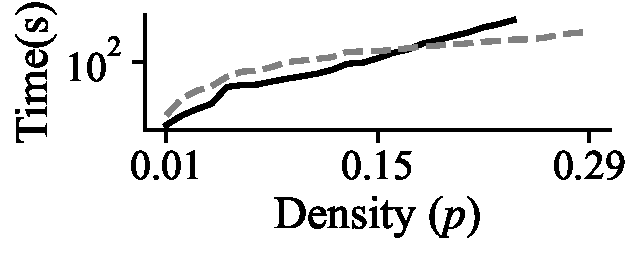
\includegraphics[width=\linewidth]{figure/runtime_r4_s5.pdf}
      \caption{r4 \\ s5}
    \end{subfigure}\hfill
    \begin{subfigure}[t]{0.24\linewidth}
      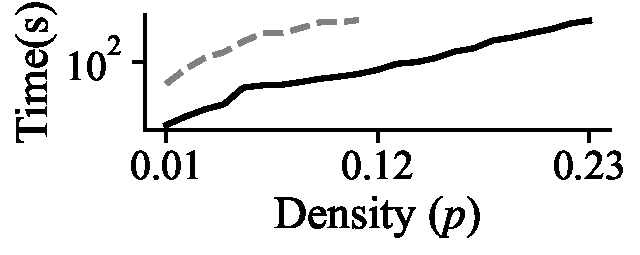
\includegraphics[width=\linewidth]{figure/runtime_r4_s6.pdf}
      \caption{r4 \\ s6}
    \end{subfigure}\hfill
    \begin{subfigure}[t]{0.24\linewidth}
      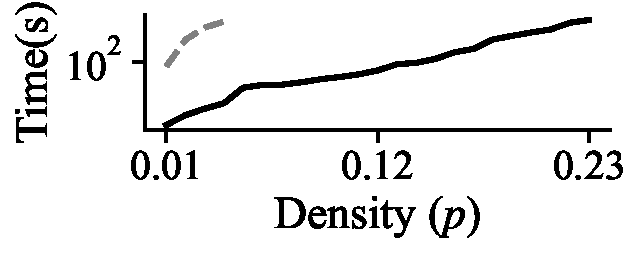
\includegraphics[width=\linewidth]{figure/runtime_r4_s7.pdf}
      \caption{r4 \\ s7}
    \end{subfigure}\hfill
    \begin{subfigure}[t]{0.24\linewidth}
      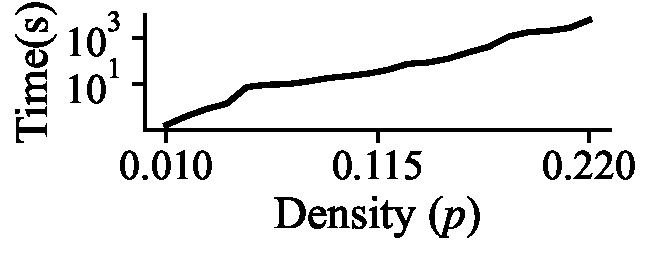
\includegraphics[width=\linewidth]{figure/runtime_r4_s8.pdf}
      \caption{r4 \\ s8}
    \end{subfigure}\hfill
    \begin{subfigure}[t]{0.24\linewidth}
      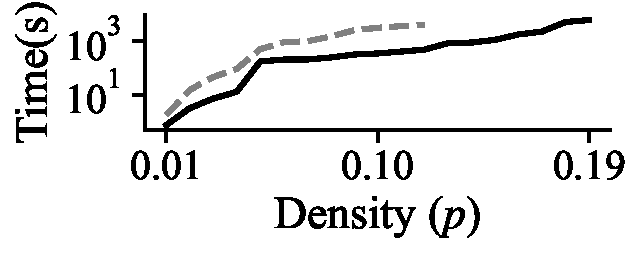
\includegraphics[width=\linewidth]{figure/runtime_r5_s6.pdf}
      \caption{r5 \\ s6}
    \end{subfigure}\hfill
    \begin{subfigure}[t]{0.24\linewidth}
      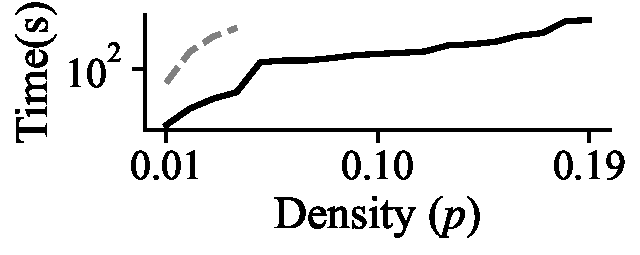
\includegraphics[width=\linewidth]{figure/runtime_r5_s7.pdf}
      \caption{r5 \\ s7}
    \end{subfigure}\hfill
    \begin{subfigure}[t]{0.24\linewidth}
      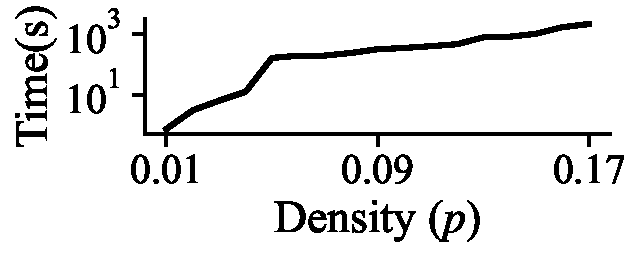
\includegraphics[width=\linewidth]{figure/runtime_r5_s8.pdf}
      \caption{r5 \\ s8}
    \end{subfigure}\hfill
    \begin{subfigure}[t]{0.24\linewidth}
      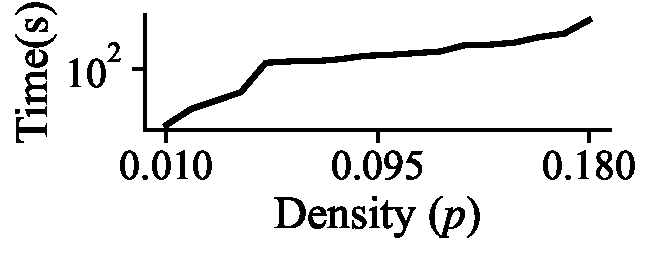
\includegraphics[width=\linewidth]{figure/runtime_r5_s9.pdf}
      \caption{r5 \\ s9}
    \end{subfigure}
  \end{minipage}
  
  

        \begin{minipage}[c]{0.02\textwidth}
    \centering
        % \raisebox{3em}{\rotatebox{90}{\tiny \textbf{Memory (Mb)}}}
  \end{minipage}  \hfill
  \begin{minipage}[c]{1\textwidth}
    \centering
    \begin{subfigure}[t]{0.24\linewidth}
      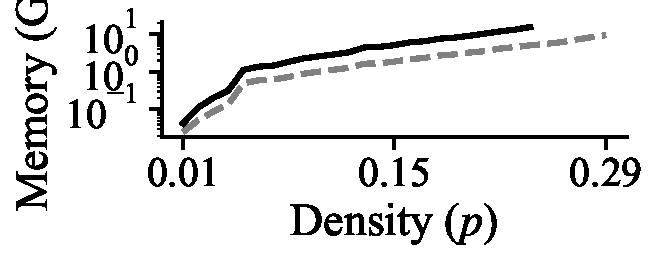
\includegraphics[width=\linewidth]{figure/memory_r4_s5.pdf}
      \caption{r4 \\ s5}
    \end{subfigure}\hfill
    \begin{subfigure}[t]{0.24\linewidth}
      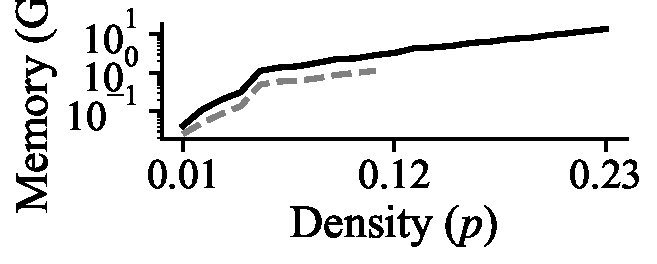
\includegraphics[width=\linewidth]{figure/memory_r4_s6.pdf}`'
      \caption{r4 \\ s6}
    \end{subfigure}\hfill
    \begin{subfigure}[t]{0.24\linewidth}
      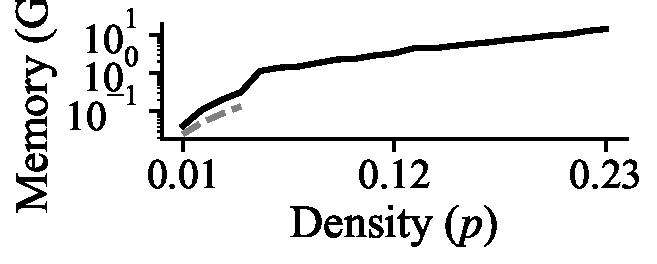
\includegraphics[width=\linewidth]{figure/memory_r4_s7.pdf}
      \caption{r4 \\ s7}
    \end{subfigure}\hfill
    \begin{subfigure}[t]{0.24\linewidth}
      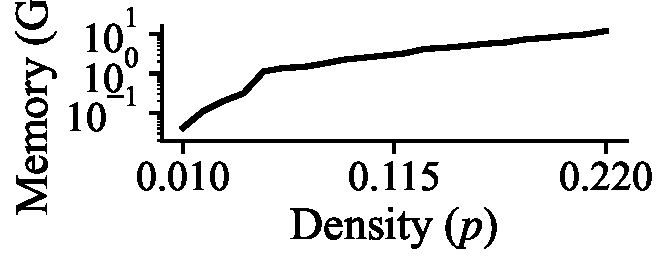
\includegraphics[width=\linewidth]{figure/memory_r4_s8.pdf}
      \caption{r4 \\ s8}
    \end{subfigure}\hfill
    \begin{subfigure}[t]{0.24\linewidth}
      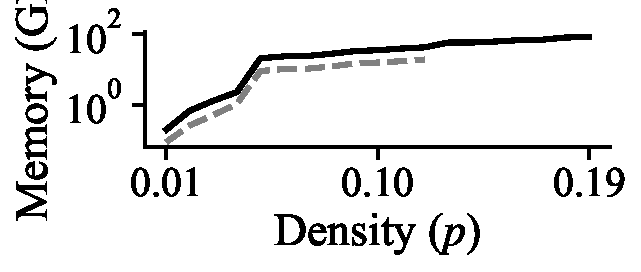
\includegraphics[width=\linewidth]{figure/memory_r5_s6.pdf}
      \caption{r5 \\ s6}
    \end{subfigure}\hfill
    \begin{subfigure}[t]{0.24\linewidth}
      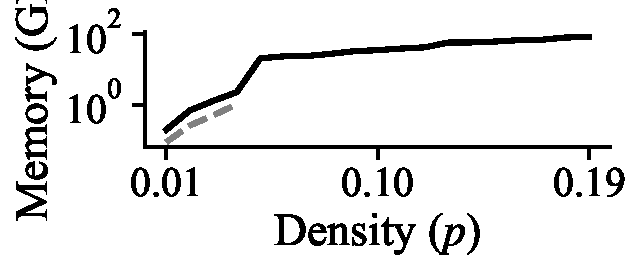
\includegraphics[width=\linewidth]{figure/memory_r5_s7.pdf}
      \caption{r5 \\ s7}
    \end{subfigure}\hfill
    \begin{subfigure}[t]{0.24\linewidth}
      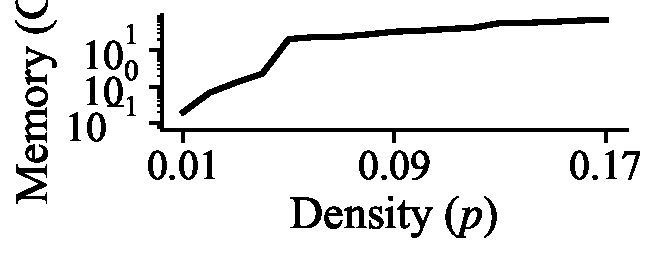
\includegraphics[width=\linewidth]{figure/memory_r5_s8.pdf}
      \caption{r5 \\ s8}
    \end{subfigure}\hfill
    \begin{subfigure}[t]{0.24\linewidth}
      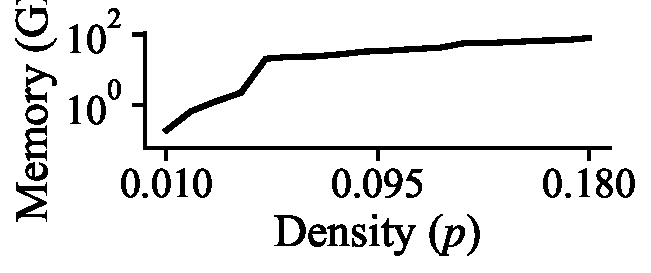
\includegraphics[width=\linewidth]{figure/memory_r5_s9.pdf}
      \caption{r5 \\ s9}
    \end{subfigure}
    
  \end{minipage}

  
  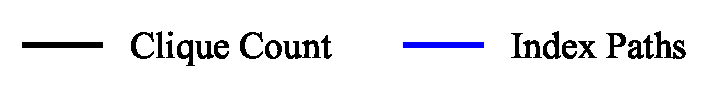
\includegraphics[width=0.4\textwidth]{figure/legend_leaf_clique.pdf}
  

  % \begin{minipage}[c]{0.02\textwidth}
  %   \centering
  %   % \raisebox{3em}{\rotatebox{90}{\tiny \textbf{Count}}}
  % \end{minipage}  \hfill
  \begin{minipage}[c]{1\textwidth}
    \centering
    \begin{subfigure}[t]{0.24\linewidth}
      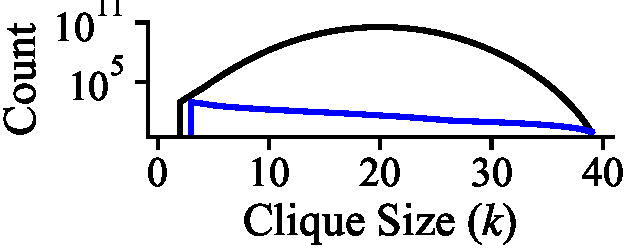
\includegraphics[width=\linewidth]{figure/snapshot_p0.01.pdf}
      \caption{p=0.01}
    \end{subfigure}\hfill
    \begin{subfigure}[t]{0.24\linewidth}
      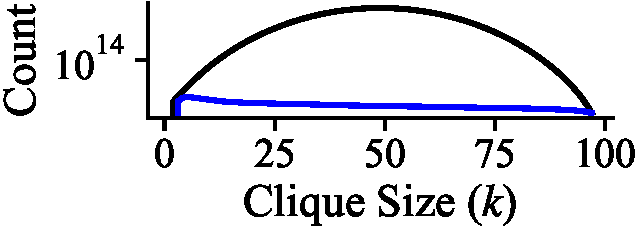
\includegraphics[width=\linewidth]{figure/snapshot_p0.06.pdf}
      \caption{p=0.06}
    \end{subfigure}\hfill
    \begin{subfigure}[t]{0.24\linewidth}
      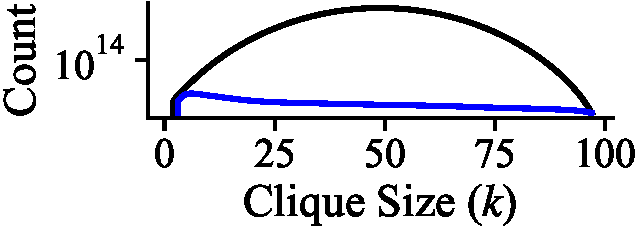
\includegraphics[width=\linewidth]{figure/snapshot_p0.11.pdf}
      \caption{p=0.11}
    \end{subfigure}\hfill
    \begin{subfigure}[t]{0.24 \linewidth}
      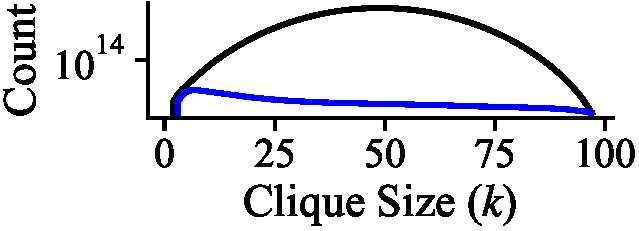
\includegraphics[width=\linewidth]{figure/snapshot_p0.16.pdf}
      \caption{p=0.16}
    \end{subfigure}\hfill
    \begin{subfigure}[t]{0.24\linewidth}
      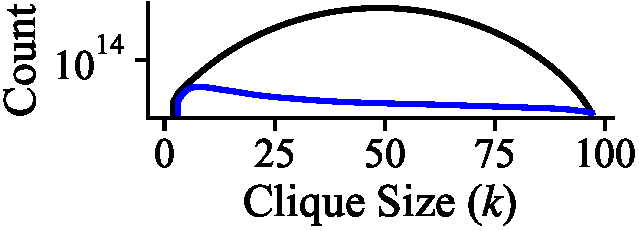
\includegraphics[width=\linewidth]{figure/snapshot_p0.22.pdf}
      \caption{p=0.22}
    \end{subfigure}\hfill
    \begin{subfigure}[t]{0.24\linewidth}
      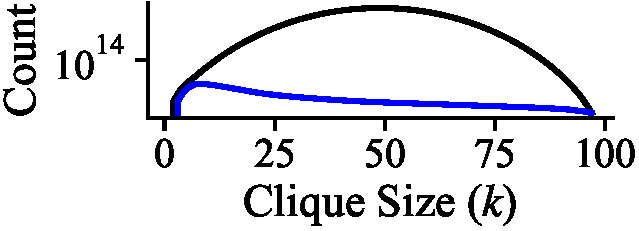
\includegraphics[width=\linewidth]{figure/snapshot_p0.27.pdf}
      \caption{p=0.27}
    \end{subfigure}\hfill
    \begin{subfigure}[t]{0.24\linewidth}
      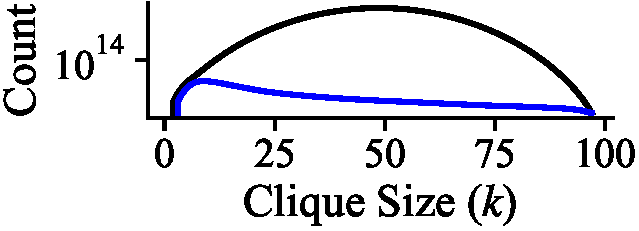
\includegraphics[width=\linewidth]{figure/snapshot_p0.32.pdf}
      \caption{p=0.32}
    \end{subfigure}\hfill
    \begin{subfigure}[t]{0.24\linewidth}
      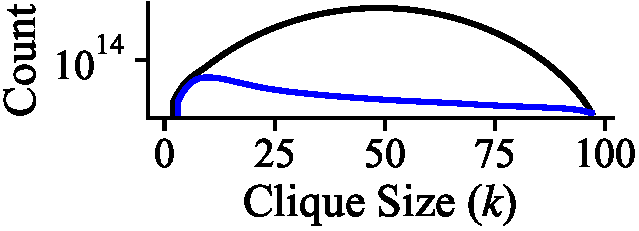
\includegraphics[width=\linewidth]{figure/snapshot_p0.38.pdf}
      \caption{p=0.38}
    \end{subfigure}
  \end{minipage}

  \caption{Comprehensive Stress Test Analysis. 
  \textbf{(a-h)} Runtime comparison across various $(r,s)$ pairs; 
  \textbf{(i-p)} Memory usage comparison corresponding to the top row; 
  \textbf{(q-x)} Leaf clique counts across varying densities ($p$).
  }
  \label{fig:stress_test_combined}
  
\end{figure}

\myaddRA{




% \begin{figure}[t]
%     \centering
    % 左侧部分：soc-pokec
    \begin{figure}
        \centering
        
\includegraphics[width=0.8\linewidth,trim=180pt 25pt 180pt 25pt,clip]{figure/pokec_fused_legend.pdf}%
        \vspace{0.3em}
        
        % 这里合并原来的子图，或者只放一张主图
        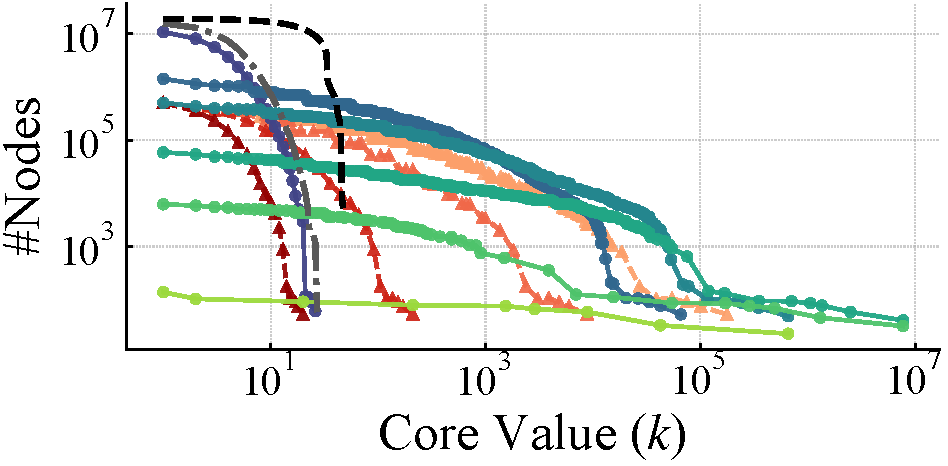
\includegraphics[width=0.47\linewidth]{figure/pokec_fused_nodes.pdf}
        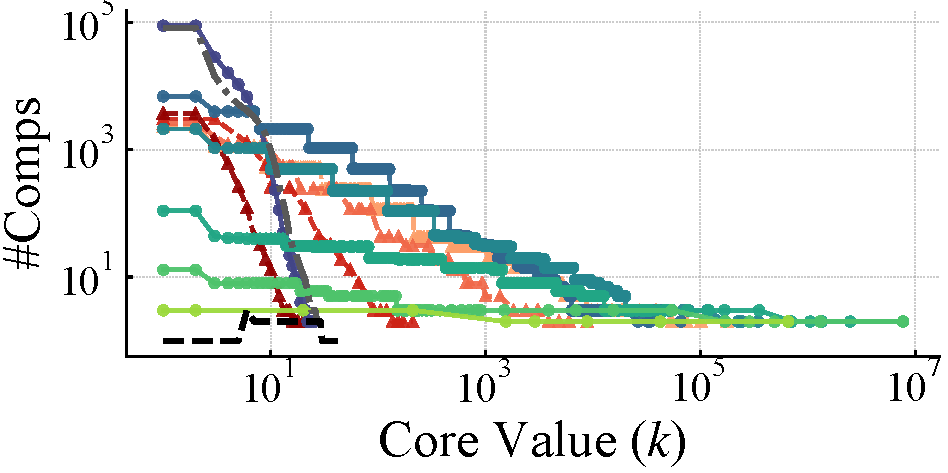
\includegraphics[width=0.47\linewidth]{figure/pokec_fused_comps.pdf}
        
        \captionof{figure}{Case study on \texttt{soc-pokec}. Solid (o): varying $s$; dashed ($\triangle$): varying $r$.}
        \label{fig:pokec-fused}
    \end{figure}

    % 右侧部分：collaborative network
    \begin{figure}
        \centering
        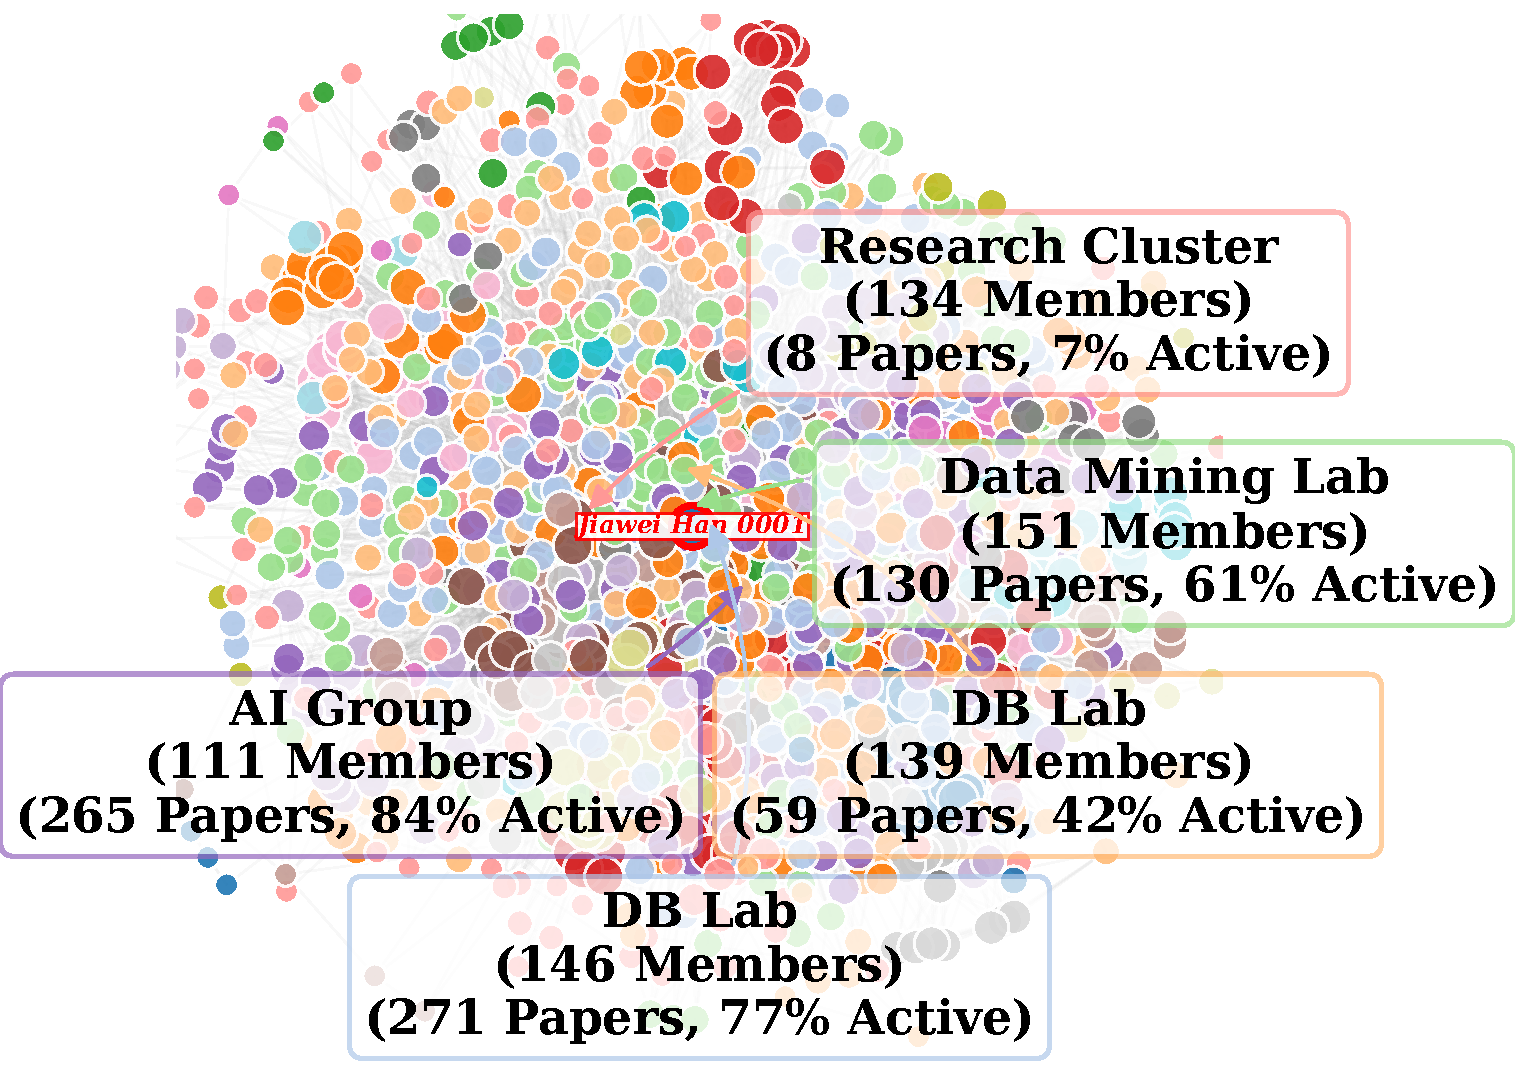
\includegraphics[width=0.47\linewidth]{figure/viz_collab_r3_s4.pdf} 
        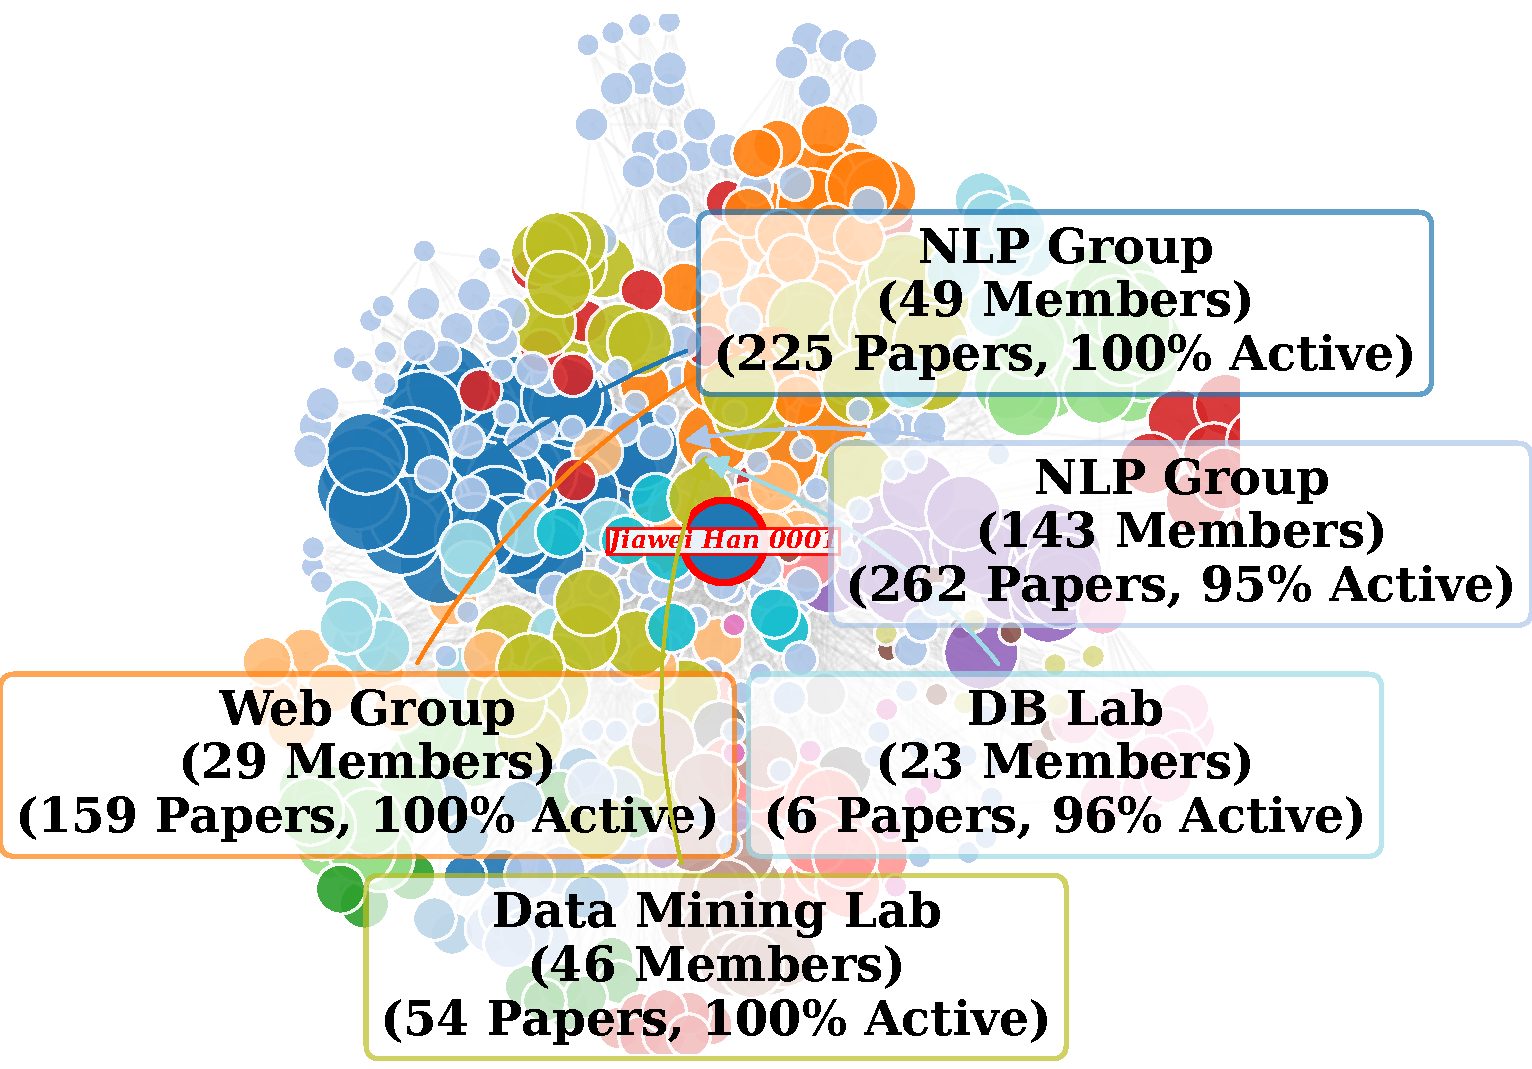
\includegraphics[width=0.47\linewidth]{figure/viz_collab_r3_s10.pdf} 
        
        \captionof{figure}{Case Study on Collaborative network: (a) Low Quality, (b) High Purity.}
        \label{fig:han-ego}
    \end{figure}
% \end{figure}

% \expsection{Case Study I: Parameter Sensitivity on \texttt{soc-pokec}}
% \label{sec:case-study-pokec}
% % 
% We examine how the two parameters---clique order $r$ and support threshold $s$---control the granularity of $(r,s)$-nucleus cores on \texttt{soc-pokec}.
% For each core value $k$ along the decomposition, we report (i) the number of surviving vertices (\texttt{living\_nodes})
% and (ii) the number of connected components (\texttt{components}) in the remaining nucleus subgraph.
% We include $k$-core ($r{=}1$) and $k$-truss ($r{=}2$) as standard baselines.

% \expsubsection{Varying $r$ under fixed $s$.}
% Fixing $s{=}10$, increasing $r$ provides limited and sometimes unstable simplification at typical operating points.
% At $k\ge 10$, moving from $r{=}3$ to $r{=}6$ reduces surviving vertices only from 319,139 to 233,661 ($1.37\times$),
% while the number of components slightly increases from 495 to 543.
% Even at a stronger threshold $k\ge 100$, $r{=}3$ retains 185,748 vertices with 226 components, whereas $r{=}6$ retains 52,041 vertices with 43 components.

% \expsubsection{Varying $s$ under fixed $r$.}
% Fixing a moderate clique order $r{=}3$, increasing $s$ yields order-of-magnitude pruning at the \emph{same} core threshold.
% At $k\ge 10$, the surviving vertices drop from 319,139 ($s{=}10$) to 42,435 ($s{=}14$) and further to 4,828 ($s{=}18$),
% while components drop from 495 to 40 and 8, respectively.
% The same trend holds at $k\ge 100$: 185,748 ($s{=}10$) $\rightarrow$ 22,017 ($s{=}14$) $\rightarrow$ 2,867 ($s{=}18$) vertices,
% and 226 $\rightarrow$ 20 $\rightarrow$ 5 components.

% \sstitle{Practical guideline (size-driven tuning).}
% We further quantify usability by the minimum core value $k_{\min}$ needed to obtain a compact subgraph.
% For $r{=}3$, achieving $\le 10{,}000$ vertices requires $k_{\min}{=}9714$ at $s{=}10$, but only $k_{\min}{=}1431$ at $s{=}14$,
% and already $k_{\min}{=}1$ at $s{=}18$ (6,252 vertices).
% Overall, on \texttt{soc-pokec}, tuning $s$ is a substantially more effective knob than tuning $r$ for distilling large cores into compact,
% well-structured modules; we thus recommend fixing a moderate $r$ (e.g., $r{=}3$) and using $s$ to control granularity.

\expsection{Case Study I: Parameter Sensitivity on \texttt{soc-pokec}}
\label{sec:case-study-pokec}
We study how $r$ and $s$ control the granularity of $(r,s)$-nucleus cores on \texttt{soc-pokec} (Figure~\ref{fig:pokec-fused}).
For each core value $k$, we report the number of surviving vertices and connected components in the remaining nucleus subgraph, and include $k$-core ($r{=}1, s{=}2$) and $k$-truss ($r{=}2, s{=}3$) as baselines.
Since the absolute scale of $k$ varies across $(r,s)$, we compare different settings mainly at the same \emph{rank} of $k$ along each curve.

\sstitle{Varying $r$ with fixed $s$.}
With $s{=}10$, at the 25\%-$k$ rank, $r{=}3$ keeps 141{,}392 vertices with 110 components, while $r{=}6$ keeps 148{,}295 vertices but increases to 245 components.

\sstitle{Varying $s$ with fixed $r$.}
Fix $r{=}3$ and increase $s$ from 10 to 14 to 18.
At the 10\%-$k$ rank (a typical operating regime), the remaining subgraph shrinks from
195{,}278 vertices / 226 components ($s{=}10$) to
32{,}310 / 30 ($s{=}14$) and further to
5{,}009 / 8 ($s{=}18$).
At the median $k$ rank, vertices drop from
78{,}233 / 41 ($s{=}10$) to
11{,}325 / 14 ($s{=}14$) and
2{,}867 / 5 ($s{=}18$).

\sstitle{$k$-core and $k$-truss (low-order baselines).}
At the 10\%-$k$ rank, $k$-core retains $18{,}449{,}233$ vertices in a single component, which is too coarse to separate modules.
$k$-truss retains $10{,}138{,}083$ vertices but yields $14{,}286$ components, indicating that low-order $(2,3)$ support admits many residual structures.
By contrast, $(r,s)=(3,10)$ at the same rank retains $195{,}278$ vertices and $226$ components, producing substantially more compact and well-structured modules.


\sstitle{The benefit of tuning $s$.}
Increasing $s$ reduces both the surviving size and the number of components, producing compact and well structured modules. It theoretically filters out incidental structures.


\sstitle{Practical guideline.}
We recommend fixing a moderate $r$ (e.g., $r{=}3$) and tuning $s$ to control granularity.
% 但是当s过大的时候, 图中获取的信息可能会过少, 例如在s=22的情况下, 大部分的节点都被删除了, 只剩下非常少的节点和连通分量.
% When $s$ is too large, close to the maximum clique size(29), the remaining subgraph may become too small to be informative (e.g., at $s{=}22$, 
When $s$ is too large(s=22), close to the dataset's maximum clique size (29), very few $s$-cliques exist and the remaining subgraph may become too small to be informative, most nodes are removed, leaving only a few nodes and components.




% \expsection{Case Study II: Ego Network of Jiawei Han on DBLP}
% \label{sec:case-study-han}
% We study a real collaboration ego network centered at Jiawei Han (1-hop coauthor graph).
% Using fixed clique order $r{=}3$, we compare two support thresholds ($s{=}4$ vs.\ $s{=}10$).
% A node is considered \emph{surviving} if its nucleus core value is positive; nodes are colored by the connected nucleus component (\texttt{cluster\_id}).
% For each component $C$, we further quantify collaboration strength using the DBLP paper list:
% a paper is counted as \emph{collaborative within $C$} if it contains at least
% $\tau(C)=\min\{5,\max(3,\lfloor 0.1|C|\rfloor)\}$ authors from $C$; the participation ratio is the fraction of members that appear in such papers.

% \ssstitle{Large $s$ yields compact and well-separated collaboration modules.}
% Increasing $s$ from 4 to 10 reduces the surviving subgraph from 1,328 to 540 nodes (59.3\%) and from 65 to 27 components (58.5\%),
% while the fraction of intra-component edges increases from 0.319 to 0.528.
% Structural quality improves substantially: the size-weighted average separability $m_{\mathrm{in}}/m_{\mathrm{cut}}$
% increases from 0.270 to 0.750, and conductance $m_{\mathrm{cut}}/(2m_{\mathrm{in}}+m_{\mathrm{cut}})$ drops from 0.712 to 0.475.

\expsection{Case Study II: Identifying ego network on DBLP.}
\label{sec:case-study-han}
We study Jiawei Han's 1-hop coauthor ego graph on DBLP and compare $s{=}4$ vs.\ $s{=}10$ under $r{=}3$.
In Fig.~\ref{fig:han-ego}, nodes are colored by nucleus component and we annotate the top-$5$ largest ones.
For each surviving component $C$, let $m_{\mathrm{in}}$ be the number of internal edges and $m_{\mathrm{cut}}$ the number of edges from $C$ to other surviving components.
We report $\phi(C)=m_{\mathrm{cut}}/(2m_{\mathrm{in}}+m_{\mathrm{cut}})$ and $m_{\mathrm{in}}/m_{\mathrm{cut}}$; lower $\phi(C)$ and higher $m_{\mathrm{in}}/m_{\mathrm{cut}}$ indicate better separation.
Using DBLP paper lists restricted to this ego network, a paper is \emph{collaborative} for $C$ if it contains $\ge3$ authors from $C$, and the \emph{active ratio} is the fraction of members appearing in at least one collaborative paper.


\sstitle{Larger $s$ yields compact and better-separated modules.}
Increasing $s$ from $4$ to $10$ shrinks the surviving subgraph from $1{,}328$ to $540$ nodes and reduces components from $65$ to $27$,
while increasing the intra-component edge fraction from $0.319$ to $0.528$.
The size-weighted average separability improves from $0.270$ to $0.750$, and the conductance score drops from $0.712$ to $0.475$,
showing that larger $s$ produces more cleanly separated collaboration modules.

\sstitle{Larger $s$ preserves highly active.}
Under the same collaboration threshold (3 within-component coauthors), the top-$5$ annotated components at $s{=}4$
have an average active ratio of $54.25\%$, and already exhibit a clear long tail (e.g., a $134$-member component has only $8$ collaborative papers and $7\%$ active members).
In contrast, at $s{=}10$ the top-$8$ components have an average active ratio of $98.15\%$; most are near $100\%$ active, with the smallest $95\%$.
This indicates that increasing $s$ filters loosely coordinated/noisy groups and retains compact, strongly collaborating teams that are easier to interpret.



% improving separability from $0.326$ to $0.666$.
% Overall, among components with at least one collaborative paper, node-level participation increases from $0.650$ to $0.901$,
% and the node share with participation $\ge 0.8$ rises from $0.453$ to $0.732$,
% supporting that tuning $s$ is an effective knob for extracting compact and interpretable collaboration cores.

}
% \section{Related Work} \label{sec:related_work}

% Cohesive subgraph discovery is a fundamental problem in graph mining, with numerous models proposed to capture various notions of cohesiveness. 
% One of the most widely used models is $k$-core decomposition~\cite{seidman1983network,zhang2023efficient,peel_cd,core_res1,kcore_4,io-eff,k-core3,core_res3,HyperCD}, which identifies dense regions in a subgraph by recursively removing vertices with degrees less than $k$, 
% Another popular model is $k$-truss decomposition~\cite{cohen2008trusses,tian2023truss,xu2022truss,chen2020truss,wang2012truss,wang2022truss,akbas2017truss,huang2014truss}, which uncovers tightly connected regions in a subgraph by recursively removing edges with support less than $k$, where the support of an edge is defined as the number of triangles containing that edge. 
% % 
% Nuclear decomposition is first introduced by \cite{firstNucleus}, which generalizes the well-known $k$-core($1,2$) and $k$-truss($2,3$) decompositions to higher-order $(r,s)$-nucleus relationships.
% Other works on nucleus decomposition have been discussed in previous sections and will not be repeated here.

% \myadd{
% Beyond core/truss-style peeling, dense subgraph mining and quasi-clique discovery study (near-)cliques under density-based objectives or relaxed constraints~\cite{Lanciano2024DensestSurvey,Konar2024OQC}. 
% These formulations are complementary to $(r,s)$-nuclei: while dense-subgraph/quasi-clique methods target an objective-driven dense subgraph (or a set of near-cliques), $(r,s)$-nucleus decomposition is defined via higher-order clique containment and support and produces a global hierarchy across core values.

% A closely related direction is community search, which is query-dependent and aims to return a cohesive subgraph containing given query vertices~\cite{SozioGionisKDD2010,SunPVLDB2025GICS}. 
% Compared to decomposition, community search focuses on answering per-query results efficiently (often with additional user constraints such as size, connectivity, or interactivity), whereas our work studies the global $(r,s)$-nucleus decomposition and targets efficient peeling with dynamic index updates.

% Finally, clique enumeration and clique counting are fundamental primitives in graph mining and are frequently used as building blocks for higher-order cohesiveness measures. 
% Recent work has revisited scalable $k$-clique counting by combining exact counting with sampling-based techniques to handle large graphs~\cite{YeSIGMOD2022Lightning}. 
% }

% \section{Conclusion and future work} \label{sec:conclusion}
% In this paper, we revisited nucleus decomposition and presented the first \textit{counting-based} framework that eliminates explicit $s$-clique enumeration.
% At the core of our approach is the \textit{Clique Path Index} (\cpi), a compact auxiliary structure that organizes the $s$-clique search space and enables direct counting, efficient dynamic updates, and connectivity maintenance throughout decomposition.
% Extensive experiments show that our method significantly accelerates both nucleus decomposition and hierarchy construction, while scaling effectively to larger $s$ values.

% \myadd{
% Our counting-and-indexing viewpoint suggests several natural directions for future work.
% First, it is well-suited for parallelization since the computations are largely local and additive: \textsc{BuildIndex} and \textsc{InitialCounting} can be parallelized by partitioning pivot vertices (or seed $r$-cliques), because CPI path generation and local support contributions are independent and can be merged via a final reduction; during peeling, \textsc{UpdateIndex}/\textsc{UpdateSupport} can be parallelized by processing removed $r$-cliques in batches with thread-local buffers and aggregated (atomic) support updates.
% More broadly, the same principle is not tied to cliques: a \emph{clique} is a vertex set where every pair is connected~\cite{diestel2000graph}, and CPI serves to index how smaller patterns are contained in larger supporting patterns so that supports can be updated by counting.
% This abstraction extends to richer graph classes by replacing cliques with an appropriate ``complete group pattern'', e.g., bicliques for bipartite graphs (closely related to $(\alpha,\beta)$-core models)~\cite{tian2024abcore}, hyperedge-induced group patterns for hypergraphs~\cite{HyperCD}, and temporal $\Delta$-cliques for temporal graphs~\cite{viard2016deltaclique}.
% We leave optimized multi-threaded implementations and these extensions as future work.
% }

% \section{Related Work} \label{sec:related_work}

% Cohesive subgraph discovery is fundamental in graph mining. 
% Classic peeling-based models include $k$-core decomposition~\cite{seidman1983network,zhang2023efficient,peel_cd,core_res1,kcore_4,io-eff,k-core3,core_res3,HyperCD}, which recursively removes vertices with degree $<k$, and $k$-truss decomposition~\cite{cohen2008trusses,tian2023truss,xu2022truss,chen2020truss,wang2012truss,wang2022truss,akbas2017truss,huang2014truss}, which recursively removes edges whose support (the number of triangles containing the edge) is $<k$. 
% Nuclear decomposition was introduced by~\cite{firstNucleus}, generalizing $k$-core($1,2$) and $k$-truss($2,3$) to higher-order $(r,s)$-nucleus relationships; other nucleus-decomposition works have been discussed earlier and are not repeated.

% \myadd{
% Beyond core/truss-style peeling, dense subgraph mining and quasi-clique discovery consider (near-)cliques under density objectives or relaxed constraints~\cite{Lanciano2024DensestSurvey,Konar2024OQC}. 
% They are complementary to $(r,s)$-nuclei: dense-subgraph/quasi-clique methods target objective-driven dense subgraphs (or sets of near-cliques), while $(r,s)$-nucleus decomposition is defined via higher-order clique containment/support and yields a global hierarchy across core values.

% Community search is query-dependent, returning a cohesive subgraph containing given query vertices~\cite{SozioGionisKDD2010,SunPVLDB2025GICS}. 
% It emphasizes efficient per-query answers (often with constraints such as size, connectivity, or interactivity), whereas we study global $(r,s)$-nucleus decomposition and focus on efficient peeling with dynamic index updates.

% Finally, clique enumeration/counting are key primitives for higher-order cohesiveness measures; recent work revisits scalable $k$-clique counting by combining exact counting with sampling to handle large graphs~\cite{YeSIGMOD2022Lightning}.
% }

% \section{Conclusion and future work} \label{sec:conclusion}
% In this paper, we revisited nucleus decomposition and presented the first \textit{counting-based} framework that eliminates explicit $s$-clique enumeration.
% Our key structure is the \textit{Clique Path Index} (\cpi), which organizes the $s$-clique search space to enable direct counting, efficient dynamic updates, and connectivity maintenance during decomposition.
% Extensive experiments show substantial speedups for both decomposition and hierarchy construction, and strong scalability to larger $s$.

% \myadd{
% Our counting-and-indexing viewpoint also suggests natural future directions.
% First, it is amenable to parallelization since computations are largely local and additive: \textsc{BuildIndex} and \textsc{InitialCounting} can parallelize over pivot vertices (or seed $r$-cliques), where CPI path generation and local support contributions are independent and merged by a final reduction; during peeling, \textsc{UpdateIndex}/\textsc{UpdateSupport} can process removed $r$-cliques in batches using thread-local buffers with aggregated (atomic) support updates.

% More broadly, the principle is not tied to cliques. 
% A \emph{clique} is a vertex set with all pairs connected~\cite{diestel2000graph}, and CPI’s role is to index how smaller patterns are contained in larger supporting patterns so that supports are updated by counting. 
% This abstraction extends to richer graph classes by replacing cliques with suitable ``complete group patterns'': bicliques for bipartite graphs (closely related to $(\alpha,\beta)$-core models)~\cite{tian2024abcore}, hyperedge-induced group patterns for hypergraphs~\cite{HyperCD}, and temporal $\Delta$-cliques for temporal graphs~\cite{viard2016deltaclique}. 
% We leave optimized multi-threaded implementations and these extensions as future work.
% }



\section{Related Work} \label{sec:related_work}

Cohesive subgraph discovery is fundamental in graph mining. 
Classic peeling-based models include $k$-core decomposition~\cite{seidman1983network,zhang2023efficient,peel_cd,core_res1,kcore_4,io-eff,k-core3,core_res3,HyperCD}, which removes vertices with degree $<k$, and $k$-truss decomposition~\cite{cohen2008trusses,tian2023truss,xu2022truss,chen2020truss,wang2012truss,wang2022truss,akbas2017truss,huang2014truss}, which removes edges whose triangle support is $<k$. 
Nucleus decomposition was introduced by~\cite{firstNucleus}, generalizing $k$-core($1,2$) and $k$-truss($2,3$) to $(r,s)$-nuclei; other nucleus-decomposition works are discussed earlier and not repeated.
%
\myaddRC{
At the exact algorithm level, prior nucleus methods mainly differ in how they handle local clique structure during support updates.
%
Some methods maintain explicit clique incidence.
%
Other methods reconstruct affected local neighborhoods on demand.
%
Still, they share the same high-level peeling skeleton.
%
They also share a reconstructive support-maintenance primitive.
%
Our work differs at this point.
%
We still use the same exact decomposition paradigm.
%
However, we replace reconstructive maintenance by a two-layer design.
%
\cpi is the representation layer.
%
DPCM is the exact maintenance layer.
}
% 
\myaddRA{
Dense-subgraph mining and quasi-clique discovery target objective-driven dense regions or relaxed clique constraints~\cite{Lanciano2024DensestSurvey,Konar2024OQC}; they are complementary to $(r,s)$-nuclei, which are defined via higher-order clique containment/support and induce a global hierarchy across core values.
Community search is query-dependent, returning a cohesive subgraph containing given query vertices~\cite{SozioGionisKDD2010,SunPVLDB2025GICS}; it emphasizes efficient per-query answers (often under constraints such as size/connectivity), whereas we focus on global $(r,s)$-nucleus peeling with efficient dynamic index updates.
Finally, clique enumeration/counting are key primitives for higher-order cohesiveness; recent work revisits scalable $k$-clique counting by combining exact counting with sampling~\cite{YeSIGMOD2022Lightning,chen2025covering,yang2021huge,lai2019distributed}.
}

\section{Conclusion and future work} \label{sec:conclusion}

In this paper, we revisited nucleus decomposition through two complementary layers.
%
First, we introduced the \textit{Clique Path Index} (\cpi), a counting-based representation that eliminates explicit $s$-clique enumeration.
%
Second, we developed \emph{Differential Path Contribution Maintenance} (DPCM).
%
It updates exact supports by maintaining path-local sufficient states and differential contributions.
%
It does not reconstruct affected clique neighborhoods.
%
Together, these two layers yield exact regime-specific instantiations for $r{=}1$, $r{=}2$, and $r{\ge}3$.
%
They also preserve efficient hierarchy construction.
%
Extensive experiments show clear speedups for both decomposition and hierarchy construction.
%
They also show that our method scales to larger $s$.

\myaddRA{
Our counting-and-indexing viewpoint together with DPCM suggests natural future directions.
%
First, it is amenable to parallelization.
%
\textsc{BuildIndex} and \textsc{InitialCounting} can parallelize over pivot vertices or seed $r$-cliques with a final reduction.
%
\textsc{UpdateIndex} and \textsc{UpdateSupport} can process removed $r$-cliques in batches by using thread-local buffers and aggregated atomic updates.
%
More importantly, the DPCM formalism suggests a broader design space.
%
This design space includes new sufficient states, symbolic update operators, and regime-specific exact maintenance rules beyond the three instantiations studied here.
}
\myaddRC{
More broadly, CPI indexes the containment between small patterns and their supporting large patterns.
%
This lets us maintain supports by counting instead of explicit enumeration.
%
This idea extends beyond cliques~\cite{diestel2000graph}.
%
Possible targets include bicliques in bipartite graphs (related to $(\alpha,\beta)$-core)~\cite{tian2024abcore}, hyperedge-induced group patterns in hypergraphs~\cite{HyperCD,luo2024hierarchical,luo2025efficient}, and temporal $\Delta$-cliques~\cite{viard2016deltaclique,chen2024compressing}. 
%
We leave optimized multi-threaded implementations, richer DPCM state systems, and these extensions as future work.
}


\section{Acknowledgements}

% This work was partially supported by the NSFC Project 62302417.
Dong Wen is supported by ARC DP230101445 and ARC DE240100668.
%
Wenjie Zhang is supported by ARC DP230101445 and ARC FT210100303.
%
Xuemin Lin is supported by NSFC U2241211, NSFC U20B2046, and GuangDong Basic and Applied Basic Research Foundation 2019B1515120048.

% \section{Introduction} \label{sec:introduction}

% 
\subsection{Optimized Peeling for $r=1$}
\label{sec:opt_r1}

For $r=1$, the baseline algorithm (Algorithm~\ref{alg:RemoveNode}) removes a vertex from the CPI by mutating the tree---deleting pivot entries and updating the hash-based vertex-to-path index.
We observe that tree mutation is entirely unnecessary for $r=1$: since every update either kills a path or removes a single pivot, the support change for each remaining vertex can be computed \emph{analytically} using a closed-form binomial difference.

\stitle{Key Idea: Immutable Tree.}
Instead of modifying the tree, we maintain two per-path integer counters:
\begin{itemize}[leftmargin=*]
\item $\mathit{rp}(\TPath)$: the number of remaining pivots on path $\TPath$;
\item $\mathit{np}(\TPath) = s - |V_h(\TPath)|$: the number of pivots needed to complete an $s$-clique (fixed at initialization).
\end{itemize}
When a batch of vertices $V_{\mathrm{rm}}$ is peeled, each affected path $\TPath$ either dies (if any $v \in V_{\mathrm{rm}}$ is a hold) or has $\mathit{rp}(\TPath)$ decremented by the number of removed pivots.

\begin{theorem}[Closed-Form Support Delta for $r=1$]\label{thm:r1_delta}
Let $\TPath = (V_h, V_p)$ be a clique path with $\mathit{rp}$ remaining pivots and $\mathit{np} = s - |V_h|$.
After removing $d$ pivots from $\TPath$ (with $\mathit{np} \le \mathit{rp} - d$, i.e., the path survives), the support change for each remaining vertex $u$ is:
\[
\Delta(u) =
\begin{cases}
\binom{\mathit{rp}}{np} - \binom{\mathit{rp}-d}{np} & \text{if } u \in V_h \text{ (hold)}, \\[4pt]
\binom{\mathit{rp}-1}{np-1} - \binom{\mathit{rp}-d-1}{np-1} & \text{if } u \in V_p \text{ (surviving pivot)}.
\end{cases}
\]
If the path dies ($\mathit{np} > \mathit{rp} - d$ or a hold is removed), the full weight $\binom{\mathit{rp}}{np}$ (resp.\ $\binom{\mathit{rp}-1}{np-1}$) is subtracted.
Each delta is a single $O(1)$ table lookup.
\end{theorem}

\begin{proof}
By Lemma~\ref{lem:clique_count}, the support contribution of a hold vertex $u$ on path $\TPath$ equals $\binom{|V_p|}{np}$, since $u$ participates in every $s$-clique on $\TPath$.
After removing $d$ pivots, $|V_p|$ decreases to $\mathit{rp} - d$, and the new contribution is $\binom{\mathit{rp}-d}{np}$.
The delta follows by subtraction.
For a surviving pivot $u$, the contribution is $\binom{|V_p|-1}{np-1}$ (choosing $np-1$ other pivots), and the argument is analogous.
\end{proof}

\stitle{Algorithm.}
The optimized peeling for $r=1$ proceeds as follows.
\begin{enumerate}[leftmargin=*]
\item \textbf{Initialization.}
Build a flat CSR index mapping each vertex to the paths containing it (replacing the hash-based index).
Initialize per-path counters $\mathit{rp}(\TPath)$ and $\mathit{np}(\TPath)$.
Compute initial supports via the nCr formula and insert all vertices into a min-heap.

\item \textbf{Peeling loop.}
In each round, extract all vertices at the current minimum support level.
For each removed vertex, scan its paths via the CSR index:
if the vertex is a hold, the path dies; if a pivot, increment the path's removal counter.
Then apply the closed-form delta (Theorem~\ref{thm:r1_delta}) to all surviving vertices on affected paths,
and update the heap immediately.

\item \textbf{No tree mutation.}
The tree structure is never modified.
Dead paths are marked via a flag and skipped in future rounds.
The CSR index remains valid throughout the entire peeling process.
\end{enumerate}

\stitle{Complexity.}
Each vertex--path pair is processed at most once (when either the vertex is peeled or the path dies).
The per-pair cost is $O(1)$ (counter update + nCr lookup + heap update).
Total time: $O\bigl(\sum_{\TPath \in \cpi} |\TPath|\cdot \log |V|\bigr)$, matching the baseline asymptotically but with significantly smaller constants due to eliminating tree mutation, hash-map updates, and re-enumeration.

\begin{algorithm}[t]
\small
\small
\caption{\textsc{UpdateIndex}(r=1)}
\label{alg:RemoveNode}
\KwIn{clique path $\TPath{} = \{V_{H},V_{P}\}$, vertices to remove $V_{\mathrm{rm}}$}
\KwOut{subpaths induced after deleting $V_{\mathrm{rm}}$}
\SetKwFunction{RemoveNode}{RemoveNode}
\SetKwFunction{CountPreVertices}{$s$-CliqueCount}
\SetKwProg{Fn}{Function}{:}{}


\lIf{$|V_{rm} \cap V_{H}(\TPath)| != 0$}{
    \Return
}
% output path $(V_{Piv}(\TPath) \setminus V, V_{Hold}(\TPath))$\;
\textbf{output path }$\{ V_{H}(\TPath),V_{P}(\TPath) \setminus V_{\mathrm{rm}}\}$\;
    %

\end{algorithm}


% 
\subsection{Optimized Peeling for $r=2$}
\label{sec:opt_r2}

For $r=2$, the baseline algorithm (Algorithm~\ref{alg:removeEdge}) handles three cases:
hold--hold edges (path dies), hold--pivot edges (pivot removed), and pivot--pivot edges (path splits via residual-graph search).
We optimize the latter two cases with closed-form formulas that eliminate most residual-graph searches.

\stitle{Key Idea: Closed-Form Deltas for Case~C.}
When pivots are removed from a surviving path (hold--pivot edges or additional pivot removals), the support change for every remaining edge can be computed analytically, analogous to the $r=1$ case.

\begin{theorem}[Closed-Form Support Delta for Pivot Removal]\label{thm:r2_pivot_delta}
Let $\TPath = (V_h, V_p)$ be a clique path with $|V_p| = P$, $|V_h| = K$, and $\mathit{np} = s - K$.
After removing $d$ pivots from $\TPath$ (path survives: $\mathit{np} \le P - d$), the support change for each surviving edge $e$ is determined by its type:
\begin{itemize}[leftmargin=*]
\item \textbf{Hold--hold edge} ($e \subseteq V_h$): \quad $\Delta(e) = \binom{P}{np} - \binom{P-d}{np}$;
\item \textbf{Pivot--pivot edge} ($e \subseteq V_p$, both survive): \quad $\Delta(e) = \binom{P-2}{np-2} - \binom{P-d-2}{np-2}$;
\item \textbf{Hold--pivot edge} ($|e \cap V_h|=1$, pivot survives): \quad $\Delta(e) = \binom{P-1}{np-1} - \binom{P-d-1}{np-1}$;
\item \textbf{Edge involving a removed pivot}: \quad $\Delta(e)$ equals the full original weight (edge loses all support from this path).
\end{itemize}
Each delta is an $O(1)$ binomial-coefficient lookup.
\end{theorem}

\begin{proof}
By Lemma~\ref{lem:clique_count}, the support contribution of an edge $e = \{u,v\}$ on path $\TPath$ depends on whether $u$ and $v$ are holds or pivots.
For a hold--hold edge, both vertices appear in every $s$-clique on $\TPath$, so the contribution equals $\binom{P}{np}$; after removing $d$ pivots this becomes $\binom{P-d}{np}$.
The other cases follow by fixing one or two pivots in the binomial coefficient.
\end{proof}


\stitle{Key Idea: Analytical Single-Edge Split for Case~B.}
When exactly one pivot--pivot edge $\{u,v\}$ is removed from a path (the most common Case~B scenario), we can construct the two resulting subpaths \emph{directly} from Theorem~\ref{thm:remove_edge}(3) without invoking the residual-graph search of Algorithm~\ref{alg:removeEdge}.

\begin{theorem}[Analytical Single-Edge Split]\label{thm:r2_single_split}
Let $\TPath = (V_h, V_p)$ be a clique path and let $\{u, v\} \subseteq V_p$ be a single removed pivot--pivot edge.
The valid $s$-cliques (those not containing both $u$ and $v$) partition into two disjoint groups, each representable as a clique path:
\begin{enumerate}[leftmargin=*]
\item $\TPath_1 = (V_h,\; V_p \setminus \{v\})$: \quad $s$-cliques \textbf{not} containing $v$;
\item $\TPath_2 = (V_h \cup \{v\},\; V_p \setminus \{u, v\})$: \quad $s$-cliques containing $v$ but \textbf{not} $u$.
\end{enumerate}
The support delta for each surviving edge on each subpath is computed via the nCr formula (Lemma~\ref{lem:clique_count}) in $O(1)$ per edge.
\end{theorem}

\begin{proof}
Every valid $s$-clique either does not contain $v$ (belongs to $\TPath_1$)
or contains $v$ but not $u$ (belongs to $\TPath_2$).
These two sets are disjoint ($\TPath_1$ excludes $v$; $\TPath_2$ includes $v$)
and exhaustive (invalid cliques are exactly those containing both $u$ and $v$).
In $\TPath_2$, vertex $v$ is moved from $V_p$ to $V_h$ because every $s$-clique in this group must contain $v$.
\end{proof}

\stitle{Effectiveness.}
In practice, the single-edge case (Theorem~\ref{thm:r2_single_split}) accounts for 93--97\% of all pivot--pivot removals at small $s$ values.
Combined with the closed-form pivot-removal delta (Theorem~\ref{thm:r2_pivot_delta}),
these optimizations eliminate the residual-graph search in the vast majority of peeling steps,
reducing the per-step cost from $O(3^{d/3} \cdot |\TPath|^2)$ (residual-graph BK) to $O(|\TPath|)$ (closed-form).

\stitle{Algorithm.}
Algorithm~\ref{alg:removeEdge} is extended as follows:
after classifying each affected path into Case~A (hold--hold $\to$ path dies), Case~C (hold--pivot or pivot-only removal $\to$ closed-form delta via Theorem~\ref{thm:r2_pivot_delta}), or Case~B (pivot--pivot edges remain):
\begin{enumerate}[leftmargin=*]
\item If $|E_{\mathrm{rm}}| = 0$ after removing hold--pivot edges $\to$ output the surviving path directly.
\item If $|E_{\mathrm{rm}}| = 1$ (single pivot--pivot edge) $\to$ apply Theorem~\ref{thm:r2_single_split} to produce two subpaths analytically.
\item If $|E_{\mathrm{rm}}| \ge 2$ $\to$ fall back to the residual-graph search (Algorithm~\ref{alg:removeEdge}).
\end{enumerate}

\begin{algorithm}[t]
\small
    \small
\caption{\textsc{$(2,s)$-CND}}
\label{alg:peeling_r2}
\KwIn{Succinct Clique Tree (\sct) $\tree$, Clique size $s$}
\KwOut{Core value $\kappa_s(v)$ for every vertex $v$}
\SetKwFunction{RemoveNode}{RemoveNode}
\SetKwFunction{CountPreEdges}{$s$-CliqueCount}
\SetKwProg{Fn}{Function}{:}{}

$count\gets \CountPreEdges(\tree,2,s)$\;

build min heap $H_{\min}$ using $count$\;

$c_{min} \gets 0$\;

\While{$H_{\min}$ is not empty}{
    $e_{min} \gets \text{ExtractMin}(H_{\min})$\;
    $c_{min} \gets \max(c_{min}, count(e_{min}))$\;
    $\kappa_s(e_{min}) \gets c_{min}$\;
    \ForEach{$e \in e_{min}$}{
        % remove edge base on lemma~\ref{lem:remove_edge}
        \ForEach{leaf $\TPath$ containing $e$}{
            \text{Remove Edge $e$ from $\TPath$ based on Theorem~\ref{thm:remove_edge}}\;
        }
    }
    \ForEach{leaf $\TPath$ containing $e \in e_{min}$}{
        Update $count(e')$ and $H_{\min}$ for all edges $e' \in \TPath$
    }  

}

\Return{$\kappa_s(e)$ for all edges $e$}\;

\end{algorithm}

% 
\subsection{Optimized Peeling for $r \ge 3$}
\label{sec:opt_r3}

For $r \ge 3$, path splitting (Algorithm~\ref{alg:removeRClique}) is the computational bottleneck:
it branches over each pivot in the conflict set, yielding worst-case exponential time.
We introduce \emph{dead-path detection}---a polynomial-time test that identifies paths where no valid subpath of size $\ge s$ can survive.
When the test succeeds, we skip the exponential splitting entirely and subtract the support directly.

\stitle{Key Idea: Budgeted Hitting Set.}
Path splitting is equivalent to a \emph{budgeted hitting set} problem.
Given a set of removed $r$-cliques $C_{\mathrm{rm}} = \{C_0, \dots, C_{m-1}\}$ on path $\TPath$,
each $C_i$ induces a \emph{conflict set} $F_i = C_i \cap V_p(\TPath)$:
the pivot members that must be ``hit'' (at least one removed) to invalidate $C_i$.
The \emph{budget} is $B = |V_p(\TPath)| - (s - |V_h(\TPath)|)$: the maximum number of pivots that may be removed while the path still encodes at least one $s$-clique.

A path is \emph{dead} if and only if $\tau(\mathcal{F}) > B$, where $\tau(\mathcal{F})$ is the minimum hitting set size of the conflict family $\mathcal{F} = \{F_0, \dots, F_{m-1}\}$.
Computing $\tau$ exactly is NP-hard, but the following polynomial-time lower bounds suffice for the vast majority of practical instances.

\begin{lemma}[Forced Vertex]\label{lem:forced_v}
If a pivot vertex $v$ appears in every $r$-clique on $\TPath$ (i.e., its conflict degree equals $\binom{|\TPath|-1}{r-1}$), then $v$ must be removed in every feasible solution.
If $v$ is a hold vertex, the path is unconditionally dead.
\end{lemma}

\begin{proof}
Since $v$ belongs to every $r$-clique, every conflict set $F_i$ contains $v$.
The only way to hit all $F_i$ is to remove $v$.
If $v$ is a hold, removing it kills the path (Theorem~\ref{lem:path_vertex_remove}).
\end{proof}

\begin{lemma}[Singleton Propagation]\label{lem:singleton_v}
If $|F_i| = 1$, say $F_i = \{p\}$, then $p$ must be removed in every feasible solution.
Removing $p$ reduces the budget by one and may create new singletons in the remaining conflict sets.
Iterative propagation runs in $O(m \cdot r)$ time.
If at any point $|V_p| + |V_h| < s$, the path is dead.
\end{lemma}

\begin{proof}
A singleton conflict set has exactly one pivot.
Any hitting set must include that pivot.
After removing it, any $F_j$ containing $p$ shrinks by one, potentially becoming a new singleton.
\end{proof}

\begin{lemma}[Disjoint Packing Lower Bound]\label{lem:packing_v}
If there exist $t$ pairwise disjoint sets in $\mathcal{F}$, then any feasible hitting set has size $\ge t$.
If $t > B$, the path is dead.
A greedy algorithm finds $t$ in $O(m^2)$ time.
\end{lemma}

\begin{proof}
Each disjoint conflict set requires at least one distinct pivot to be removed.
Hence $\tau(\mathcal{F}) \ge t$.
\end{proof}

\begin{lemma}[Component Decomposition]\label{lem:component_v}
Let $G_c$ be the \emph{conflict graph} on $V_p$, where two pivots are adjacent iff they co-occur in some $F_i$.
If $G_c$ has connected components $\mathcal{C}_1, \dots, \mathcal{C}_k$, then:
\[
\tau(\mathcal{F}) = \sum_{j=1}^{k} \tau(\mathcal{F}[\mathcal{C}_j]),
\]
where $\mathcal{F}[\mathcal{C}_j]$ denotes the conflict sets restricted to component $\mathcal{C}_j$.
Computing the packing lower bound per component yields a bound $\ge$ the global packing bound.
\end{lemma}

\begin{proof}
Since no conflict set spans two components, the hitting set decomposes independently.
Per-component packing sums to at least the global packing (each disjoint pair is within one component).
\end{proof}


\stitle{Algorithm.}
These conditions are applied as a preprocessing step before the recursive path split (Algorithm~\ref{alg:removeRClique}).
Algorithm~\ref{alg:pathsplit_pruning} summarizes the pruned procedure:

\begin{enumerate}[leftmargin=*]
\item \textbf{Forced vertex detection}: remove pivots with conflict degree $= \binom{|\TPath|-1}{r-1}$.
\item \textbf{Singleton propagation}: iteratively remove singleton conflict pivots; propagate until stable.
\item \textbf{Packing + component bound}: compute per-component disjoint packing; if total $> B$, declare dead.
\item If dead: subtract support for all $r$-cliques on $\TPath$ via direct enumeration in $O\bigl(\binom{|\TPath|}{r}\bigr)$.
\item If alive: proceed with recursive path split (Algorithm~\ref{alg:removeRClique}).
\end{enumerate}


\begin{algorithm}[t]
\small
\caption{\textsc{PrunedUpdateIndex}}
\label{alg:pathsplit_pruning}
\KwIn{clique path $\TPath{} = \{V_H, V_P\}$, $r$-cliques to remove $C_{\mathrm{rm}}$, clique size $s$}
\KwOut{All subpaths after deletion, or $\emptyset$ if dead}
\SetKwFunction{Split}{PathSplit}
\SetKwProg{Fn}{Function}{}{}

$F_i \gets C_i \cap V_P$ for each $C_i \in C_{\mathrm{rm}}$\tcp*{conflict sets}
$B \gets |V_P| - (s - |V_H|)$\tcp*{removal budget}

\tcp{Forced vertex (Lemma~\ref{lem:forced_vertex})}
\ForEach{$v$ with conflict degree $\ge \binom{|\TPath|-1}{r-1}$}{
  \lIf{$v \in V_H$}{\Return $\emptyset$}
  $V_P \gets V_P \setminus \{v\}$; resolve all $F_i \ni v$\;
}

\tcp{Singleton propagation (Lemma~\ref{lem:singleton})}
\Repeat{no change}{
  \ForEach{active $F_i$ with $|F_i| = 1$, say $\{p\}$}{
    $V_P \gets V_P \setminus \{p\}$; resolve all $F_j \ni p$\;
    \lIf{$|V_H| + |V_P| < s$}{\Return $\emptyset$}
  }
}

\tcp{Component packing LB (Lemmas~\ref{lem:packing},~\ref{lem:component_lb})}
Build conflict graph $G_c$; find components $C_1, \dots, C_k$\;
$\mathit{LB} \gets \sum_{j=1}^{k} \textsc{GreedyPacking}(\{F_i \mid F_i \subseteq C_j\})$\;
\lIf{$\mathit{LB} > B$}{\Return $\emptyset$}

\Return \Split{$V_H, V_P$} with reduced $\mathcal{F}$\tcp*{Alg.~\ref{alg:removeRClique}}
\end{algorithm}



\stitle{Effectiveness.}
Table~\ref{tab:leafdeath} reports the fraction of paths detected as dead by the above tests.
On representative datasets at $s = 20$, dead-path detection prunes 95--97\% of all paths,
reducing the number of expensive recursive splits by up to $47\times$.
This is the primary reason our method completes on parameter ranges where the baseline times out.

\stitle{Complexity.}
The preprocessing (Lemmas~\ref{lem:forced_v}--\ref{lem:component_v}) runs in $O(m^2 \cdot r)$ time, where $m = |C_{\mathrm{rm}}|$.
When the path is dead, the support subtraction costs $O\bigl(\binom{|\TPath|}{r}\bigr)$---polynomial in the path size.
The exponential recursive split (Algorithm~\ref{alg:removeRClique}) is invoked only for the surviving 3--5\% of paths.


% ---- Bibliography ----
%
% BibTeX users should specify bibliography style 'splncs04'.
% References will then be sorted and formatted in the correct style.
%
% \bibliographystyle{splncs04}
% \bibliography{mybibliography}
%
\FloatBarrier

% \endlinenumbers
\newpage
\balance

\bibliographystyle{ACM-Reference-Format}
\bibliography{references}

\end{document}
